\documentclass[oneside]{book}
\usepackage{../Style/Master}
\usepackage{../Style/boxes}
\usepackage{../Style/Env}
\usepackage{../Style/DefNoteFact}
\usepackage{../Style/QnsProof}
\usepackage{../Style/Thms}
\usepackage{newpxtext, eulerpx}
\usepackage{bbding}
\begin{document}

\begin{titlepage}
    \frontmatter
    \begin{tikzpicture}[font=\sffamily,remember picture,overlay]
        \node[fill=Dandelion,anchor=north, minimum width=\paperwidth, minimum height=2cm] (names)
     at ([yshift=0]current page.north) {
      \begin{tabular}{c}
          \\
          \color{blue} {\fontsize{24.88pt}{65pt}\selectfont A-Levels Physics Notes}\\[2mm]
          \Large \color{blue}{By Grass}\\
          \color{blue} {\fontsize{10pt}{10pt}\selectfont Licensed under the GNU General Public License v3.0}\\
      \end{tabular}
      };
    \end{tikzpicture}

\begingroup
\let\clearpage\relax
\vspace{2cm}
\tableofcontents
\endgroup
\mainmatter
\end{titlepage}

\raggedright
\chapter{Kinematics}
\begin{center}
    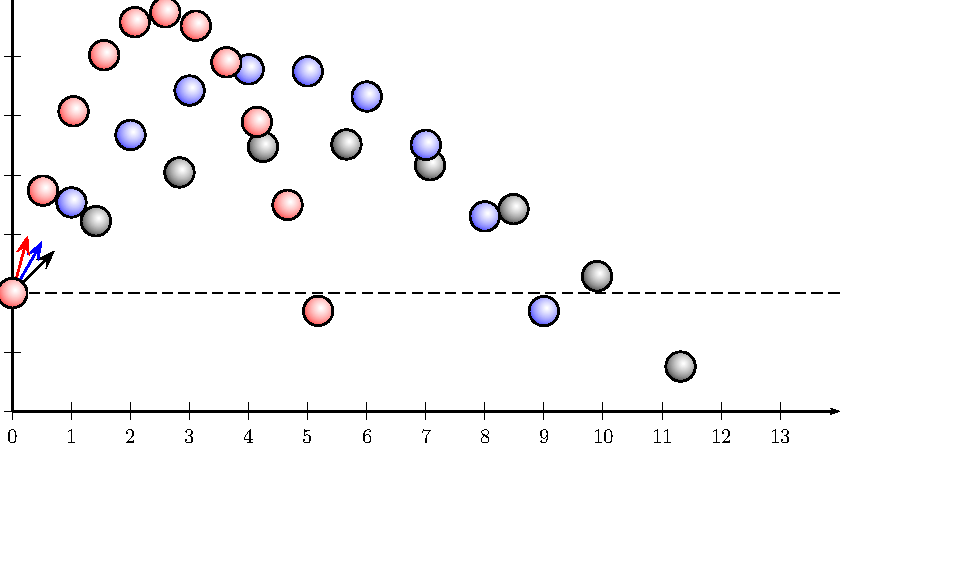
\includegraphics[width=\textwidth]{../images/Kinematics/schieferWurf.pdf}
    \captionsetup{type=figure}
    \caption[figure]{\ref{Projectile motion} Parabolic path travelled by balls thrown at varying angles.}
\end{center}
\begin{itemize}
    \item \emph{Distance} is defined as the total length of \emph{path} travelled.
    \item \emph{Displacement} is defined as the distance of a point from some reference point \emph{in a specified direction}.
    \item \emph{Velocity} is defined as the rate of change of displacement.
    \item \emph{Acceleration} is defined as the rate of change of velocity.
    \item Four key formulas for kinematics. When the  acceleration \(a\) is constant:
    \begin{enumerate}
        \item \(v=u+at\),
        \item \(s=ut+\frac{1}{2}at^2\),
        \item \(s=\frac{1}{2}(u+v)t\),
        \item \(v^2=u^2+2as\).
    \end{enumerate}
\end{itemize}
\chapter{Dynamics}
\begin{itemize}
    \item \emph{Newton's First Law of Motion} states that an object at rest will remain at rest and an object in motion will remain in motion at constant velocity in a straight line in the absence of an \emph{external} resultant force.
    \item The \emph{linear momentum} of a body is the product of its mass and velocity. The linear momentum is in the \emph{same direction} as it velocity.
    \item \emph{Newton's Second Law of Motion} states that the rate of change of momentum of a body is directly proportional to the resultant force acting on the body and occurs \emph{in the direction} of the resultant force.
    \item \emph{Newton's Third Law of Motion} states that if body A exerts a force on body B, then body B exerts a force of the \emph{same type} that is equal in magnitude and opposite in direction on body A.
    \item \emph{Impulse} is defined as the product of \emph{average} force acting on an object and the time for which the force acts.
    \item The \emph{Principle of Conservation of Linear Momentum} states that the total momentum of a system remains constant provided no \emph{external} resultant force acts on the system.
\end{itemize}
\chapter{Forces}
\begin{center}
    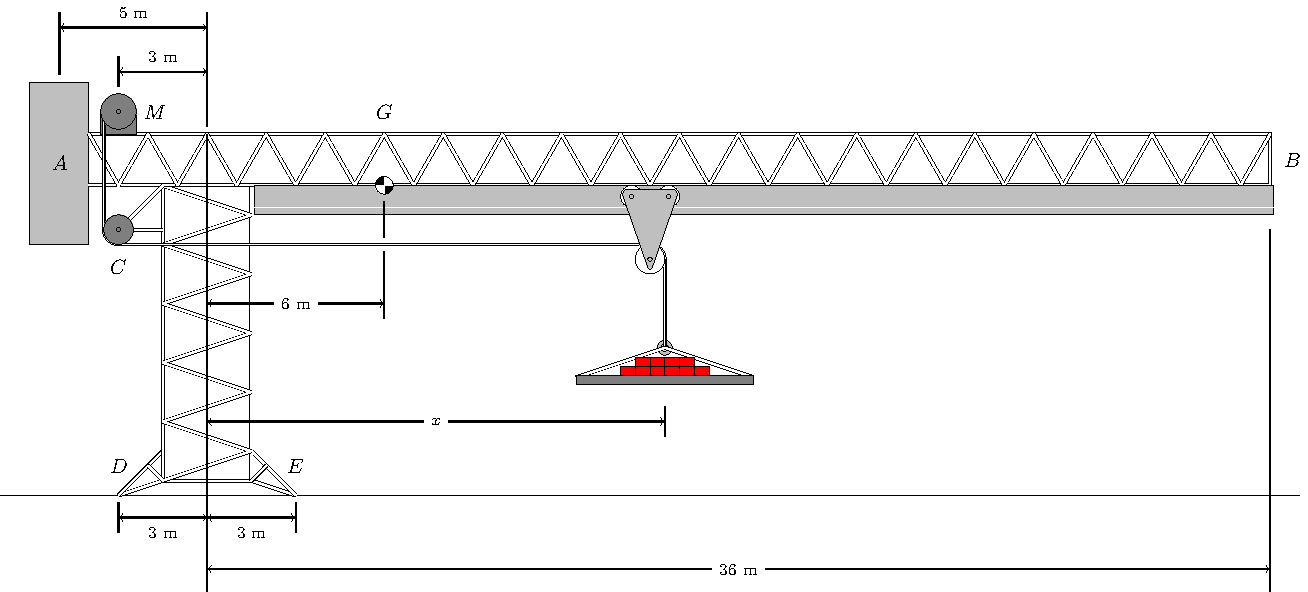
\includegraphics[width=\textwidth,page=1]{../images/Crane/Crane.pdf}
    \captionsetup{type=figure}
    \caption[figure]{\ref{Crane} Forces acting on a crane.}
\end{center}
\begin{itemize}
    \item \emph{Hooke's Law} states that the force is directly proportional to the extension in a material if its \emph{limit of proportionality} is not exceeded.
    \item The \emph{center of gravity} of an object is the point at which the entire weight of a body may be considered to act.
    \item The \emph{moment} of a force is equal to the product of the force and the \emph{perpendicular} distance of the \emph{line of action} of the force from the pivot. It is also the turning effect of a force.
    \item \emph{Torque of a couple} is defined as the product of one of the forces and the \emph{perpendicular} distance between the \emph{lines of action} of the forces.
    \item The \emph{Principle of Moments} states that if a body is in equilibrium, the sum of all the clockwise moments about \emph{any axis} must be equal to the sum of anticlockwise moments about the \emph{same axis}.
    \item \emph{Density} is defined as the mass per unit volume of a substance.
    \item \emph{Pressure} is defined as force per unit area, where the force is \emph{acting perpendicularly} to the area.
    \item Deriving \(p=\rho gh\):
    \begin{enumerate}
        \item Consider a point at a depth \(h\) below the surface of a liquid of density \(\rho\). 
        \item The force \(F\) acting perpendicularly on a surface area \(A\) at depth \(h\) is due to the weight of the liquid column above \(A\) to give pressure \(p\). Thus, \(p=\frac{F}{A}=\frac{mg}{A}=\frac{\rho Ah}{g}=\rho gh\).
    \end{enumerate}
    \item \emph{Upthrust} is the upward force exerted by a fluid on a body immersed in the fluid (due to pressure difference in the fluid).
    \item \emph{The origin of upthrust:} Upthrust is a result of the pressure difference between top and bottom surfaces of the body, resulting in a net upwards force being exerted on the body by the third medium in which the body is located.
    \item \emph{Archimedes' Principle} states that when a body is totally or partially immersed in a fluid, it experiences an upward force (upthrust) equal to the weight of fluid displaced.
    \item \emph{The Principle of Floatation} states that, for any object floating in \emph{equilibrium}, the upthrust is equal to the weight of the object.
\end{itemize}
\chapter{Work, Energy, and Power}
\begin{itemize}
    \item \emph{Work done} is defined as the product of a force and the displacement in the direction of the force.
    \item \emph{One joule of work} is defined as the work done by a force of 1 Newton when its \emph{point of application} moves through a distance of 1 metre in the direction of the force.
    \item \emph{Energy} is defined as the ability to do work.
    \item \emph{The Principle of Conservation of Energy} states that energy can neither be created or destroyed in \emph{any process}. It can be transformed from one form to another, and transferred from one body to another.
    \item Deriving \(E_k=\frac{1}{2}mv^2\): 
    \begin{enumerate}
        \item Consider a constant horizontal applied force \(F\) acting on an object of mass \(m\) travelling with initial velocity \(u\) to reach a final velocity \(v\) over a displacement \(s\). 
        \item For uniform acceleration, \(v^2=u^2+2as\) so \(as=\frac{1}{2}(v^2-u^2)\). Combined with Newton's Second Law, \(W=Fs=mas=\frac{1}{2}mv^2-\frac{1}{2}mu^2\). When the object starts from rest, \(u=0\). 
        \item By conservation of energy,\emph{ the work done by force \(F\) must be converted into the kinetic energy \(E_k\) of the object}. Hence, \(E_k=W=\frac{1}{2}mv^2-\frac{1}{2}m(0)^2=\frac{1}{2}mv^2\).
    \end{enumerate}
    \item The \emph{Work-Energy Theorem} states that the net work done by \emph{external} forces acting on a particle is equal to the change in kinetic energy of the particle.
    \item Deriving \(E_p=mgh\):
    \begin{enumerate}
        \item Consider an object from the Earth's surface --- which is taken as the reference for zero gravitational potential energy --- raised up by a \emph{constant force \(F\) equal to and opposite to the weight \(mg\)} of the object such that the object moves up at \emph{constant velocity} to a height \(h_2\). 
        \item Thus, the object moves at constant speed so \(\Delta E_k=0\). Therefore, 
        \begin{align*}
            \Delta E_p&= W\\
            E_p-0&=Fs\\
            E_p&=mgh.
        \end{align*}
        Where \(E_p\) is the gravitational potential energy at height \(h\) above the Earth's surface.
    \end{enumerate}
    \item Know how to \(\Delta E_p=\frac{1}{2}kx^2\) from area under graph.
    \item \emph{Power} is defined as the rate of doing work.
    \item Derive \(P=Fv\): \(P=\frac{\text{d}W}{\text{d}t}=\frac{F\text{d}s}{\text{d}t}=Fv\).
\end{itemize}
\chapter{Temperature and Ideal Gases}
\begin{itemize}
    \item From empirical results, we know that there appears to be a \emph{linear} trend, wherein pressure and volume decrease, when temperature decreases. So, there must be a temperature where pressure is zero, and a temperature where volume is zero. Empirical data shows that the temperature at which this occurs is the same for all gases under all experimental conditions. This temperature is known as \emph{absolute zero}.
    \item The \emph{Zeroth Law of Thermodynamics} If bodies \(A\) and \(B\) are separately in thermal equilibrium with body \(C\), then bodies \(A\) and \(B\) are in thermal equilibrium with each other.
    \item \emph{One mole} is defined as the amount of substance that contains as many elementary particles as there are atoms in 0.012kg of carbon-12.
    \item \emph{Avogadro's Constant \(N_A\)} is the number of atoms in 0.012kg of carbon-12.
    \item Celsius-Kelvin conversion: \(T\ {^\circ}\text{C}=(T+273.15)\ \text{K}\). 
    \begin{figure}[H]
        \centering
        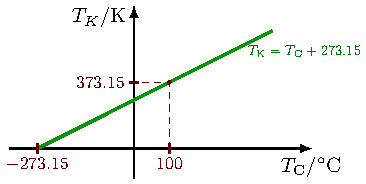
\includegraphics{../images/Celcius-Kelvin/Celcius-Kelvin.pdf}
        \caption{\ref{source:celsius-kelvin} Kelvin against celsius graph.}
        \label{fig:celsius-kelvin}
    \end{figure}
    \item There is no ideal gas in nature, but at \emph{low pressures} and \emph{high temperatures}, real gases behave like ideal gases.
    \item \emph{Boyle's Law}. When the temperature of an ideal gas remains constant, the product of its pressure \(p\) and volume \(V\) is constant. i.e. \(p_1V_1=p_2V_2\).
    \item \emph{Charles' Law}. When the pressure of an ideal gas remains constant, its volume \(V\) is directly proportional to its thermodynamic temperature \(T/K\). i.e. \(V_1/T_1=V_2/T_2\).
    \item \emph{Gay-Lussac's Law}. When the volume of an ideal gas remains constant, its pressure \(p\) is directly proportional to its thermodynamic temperature \(T/K\). i.e. \(p_1/T_1=p_2/T_2\).
    \item Let \(n\) be the amount of gas in moles and the integer \(N\) be the number of gas molecules. Then, for the molar gas constant \(R=8.31\) J K\(^{-1}\) mol\(^{-1}\) and Boltzmann's constant \(k=1.38\cdot 10^{-23}\) J K\(^{-1}\), the equation of state for an ideal gas is \(pV=nRT=NkT\).
    \item Some useful conversions: \(n=\frac{M/\text{kg}}{M/\text{mol}}=\frac{N}{N_A}\).
    \newpage
    \item ~\\[-3mm]
    \begin{tabular}{|Sc|Sl|}
        \hline
        & Assumptions of the Kinetic Theory of Gases\\
        \hline
        \textbf{M} & 
        \begin{tabular}{@{}Sl@{}}
            The molecules of the gas are in \emph{rapid} and \emph{random} motion.
          \end{tabular}\\
        \hline
        \textbf{A} & 
        \begin{tabular}{@{}Sl@{}}
            There are \emph{no intermolecular} attractive forces.
        \end{tabular}\\
        \hline
        \textbf{N} & 
        \begin{tabular}{@{}Sl@{}}
        Any gas consists of a \emph{very large number} of molecules.
        \end{tabular}\\
        \hline
        \textbf{T} & 
        \begin{tabular}{@{}Sl@{}}
        The duration of collisions is negligible compared\\ to the time interval between collisions.
        \end{tabular}\\
        \hline
        \textbf{E} & 
        \begin{tabular}{@{}Sl@{}}
        The collisions between gas molecules, and between\\ gas molecules and the container walls are \emph{perfectly elastic}.
        \end{tabular}\\
        \hline
        \textbf{V} & 
        \begin{tabular}{@{}Sl@{}}
        The volume of the gas molecules themselves is negligible \\compared to the volume of the container.
        \end{tabular}\\
        \hline
    \end{tabular}
    \item Real gases are approximately ideal at high temperatures and low pressures.
    \item Deriving \(p=\frac{1}{3}\frac{Nm}{V}\langle c^2 \rangle\) for an ideal gas:
    \begin{enumerate}
        \item Consider a cubic container of side \(l\) containing \(N\) molecules, each of mass m.
        \item Change in momentum due to \emph{elastic} collision between wall and molecule\(\text{}=2mc_x\)
        \item Time interval between collisions, \(\Delta t=\frac{2l}{c_x}\).
        \item By Newton's 2nd Law, \(F=\frac{2mc_x}{\frac{2l}{c_x}}=\frac{mc_x^2}{l}\).
        \item Since \(A=l^2\), Pressure due to 1 particle, \(p=\frac{mc_x^2}{l^3}=\frac{mc_x^2}{V}\).
        \item Pressure due to \(N\) particles, \(p_N=\frac{Nmc_x^2}{V}\).
        \item By Pythagoras'Theorem, \(c^2=c_x^2+c_y^2+c_z^2\). The average speed in the \(x\), \(y\), and \(z\) directions can be taken to be \(c_x=c_y=c_z\) so \(c^2=3c_x^2\). Now, \(p_N=\frac{Nm\langle \frac{1}{3}c^2\rangle}{V}=\frac{1}{3}\frac{Nm\langle c^2 \rangle}{V}\).
    \end{enumerate}
    \item The mean translational kinetic energy of an ideal gas molecule molecule is \(\frac{1}{2}m \langle c^2 \rangle=\frac{3}{2}kT\).
    \item The total translational kinetic energy of \(N\) ideal gas molecules is \(\frac{3}{2}NkT=\frac{3}{2}nRT=\frac{3}{2}pV\). This is valid for monoatomic gases.
\end{itemize}
\chapter{First Law of Thermodynamics}
\begin{itemize}
    \item The \emph{heat capacity} of a body is defined as the amount of thermal energy required to raise its temperature by one Kelvin / degree Celsius.
    \item The specific \emph{heat capacity} of a body is defined as the amount of thermal energy required to raise the temperature of one unit mass of the substance by one Kelvin / degree Celsius.
    \item The \emph{specific latent heat} of a body is defined as the thermal energy required to change \emph{phase} of one unit mass of a substance, \emph{without a change in temperature}.
    \item \emph{Internal energy} of a system is a sum of \emph{random distribution} of kinetic and potential energy \emph{associated with the molecules} of the system.
    \item An ideal monoatomic gas of \(N\) atoms only has translational motion and no intermolecular potential energy, \(U=E_k=N\cdot\text{translational \(E_k\) of one atom}=\frac{3}{2}NkT\).
    \item For non-monoatomic ideal gases, \(U\neq \frac{3}{2}NkT\). But we know that \(U_{\text{Total}}\propto NT\) and \(U_{\text{one molecule}}\propto T\).
    \item The \emph{First Law of Thermodynamics} states that the \emph{increase} in internal energy of a closed system is the \emph{sum} of heat \emph{supplied} to the system and the work done \emph{on} the system. i.e. \(\Delta U=Q+W\).
    \item The work done \(W\) on a gas against a constant external pressure \(p\) is such that \(W=-p\Delta V\).
    \item In general, the work done on a gas is \(W=-\int_{V_i}^{V_f}p\,dV\).
    \item An \emph{\textcolor{blue}{isothermal} process} is one that takes place without a change in temperature, i.e. \(\Delta T=0\). Thus, for an ideal gas, \(\Delta U=\frac{3}{2}Nk\Delta T=0\).
    \item An \emph{\textcolor{pink!75!red}{iso-volumetric/isochoric} process} is one that takes place without a change in volume, i.e. \(\Delta V=0\). Hence, when the external pressure is constant, \(W=0\).  
    \item An \emph{\textcolor{green!85!black}{isobaric} process} is one that takes place without a change in pressure, i.e. \(\Delta p=0\).
    \item An \emph{\textcolor{red!60!black}{adiabatic} process} is one that takes place without heat transfer, i.e. \(Q=0\). Therefore, \(Q=0\).
    \begin{figure}[H]
        \centering
        \begin{subfigure}[c]{0.30\textwidth}
            \centering
            \includegraphics[page=6]{../images/Thermodynamics/Thermodynamics.pdf}
            \caption{An \textcolor{blue}{isothermal} process.}
            \label{fig:isothermal}
        \end{subfigure}%
        \begin{subfigure}[c]{0.30\textwidth}
            \centering
            \includegraphics[page=7]{../images/Thermodynamics/Thermodynamics.pdf}
            \caption{\textcolor{pink!75!red}{Iso-volumetric} and \textcolor{green!85!black}{isobaric} processes.}
            \label{fig:iso-volumetric}
        \end{subfigure}%
        \begin{subfigure}[c]{0.30\textwidth}
            \centering
            \includegraphics[page=8]{../images/Thermodynamics/Thermodynamics.pdf}
            \caption{An An \textcolor{red!60!black}{adiabatic} process.}
            \label{fig:adiabatic}
        \end{subfigure}%
        \caption{\ref{source:thermodynamic-processes} Illustrations for isothermal, iso-volumetric/isochoric, isobaric, and adiabatic processes.}
        \label{fig:thermodynamic-processes-PV-diagram}
    \end{figure}
    \item A thermodynamic cyclic process is one that eventually returns to its initial state. 
    \begin{itemize}
        \item \(\Delta U=0\) so \(Q=-W\). 
        \item The net work done by/on the gas is given by the area enclosed by the closed loop.
    \end{itemize}
    \begin{figure}[H]
        \centering
        \begin{subfigure}[c]{0.30\textwidth}
            \centering
            \includegraphics[page=4]{../images/Thermodynamics/Thermodynamics.pdf}
            \caption{A simple engine.}
            \label{fig:simple-engine-theromdynamics-closed-loop}
        \end{subfigure}%
        \begin{subfigure}[c]{0.30\textwidth}
            \centering
            \includegraphics[page=10]{../images/Thermodynamics/Thermodynamics.pdf}
            \caption{An Otto cycle}
            \label{fig:otto-cycle-theromdynamics-closed-loop}
        \end{subfigure}%
        \begin{subfigure}[c]{0.30\textwidth}
            \centering
            \includegraphics[page=11]{../images/Thermodynamics/Thermodynamics.pdf}
            \caption{A Carnot cycle.}
            \label{fig:carnot-cycle-theromdynamics-closed-loop}
        \end{subfigure}%
        \caption{\ref{source:thermodynamic-processes} Some thermodynamic cyclic processes.}
        \label{fig:thermodynamic-cyclic-processes}
    \end{figure}
\end{itemize}

\chapter{Circular Motion}
\begin{itemize}
    \item \emph{Angular displacement} is the angle through which an object turns \emph{with respect to the center} of the circular path.
    \item \emph{The radian} is defined as the angle \emph{subtended} at the \emph{center} of a circle by an \emph{arc} of length equal to the radius of the circle. 
    \item \emph{Angular velocity} is the rate of change of angular displacement.
\end{itemize}
\begin{itemize}[label=\(\square\)]
    \item \begin{tabular}{|Sc|Sc|Sc|Sc|Sc|}
        \hline
            \(\begin{aligned}
                \omega=\frac{2\pi}{T}=2\pi f
            \end{aligned}\)&
            \(\begin{aligned}
                v=r\omega
            \end{aligned}\)&
            \(\begin{aligned}
                a_c=\frac{v^2}{r}=r\omega^2=v\omega
            \end{aligned}\)&
            \(\begin{aligned}
                F_c=ma_c
            \end{aligned}\)
        \\
        \hline
    \end{tabular}
    \item Common formulae: \(\theta=\tan^{-1}\left(\frac{v^2}{rg}\right)\), \(v=\sqrt{rg}\).
    \item Water in bucket at top position: \(F_c=N+W\) (where \(N\geq 0\)) so \(\omega>\sqrt{\frac{g}{r}}\).
    \item Need to write ``Centripetal force is provided by \underline{\hspace{1cm}}'' 
\end{itemize}
\chapter{Gravitational Fields}
\begin{itemize}
    \item \emph{Newton's Law of Gravitation} states that the force of attraction between any two point masses is directly proportional to the product of their masses and inversely proportional to the square of their separation.
    \item A \emph{gravitational field} is a region in space where mass experiences a gravitational force acting on it.
    \item Gravitational field strength at a point is defined as the gravitational force per unit mass acting on a small mass placed at that point
    \item The \emph{gravitational potential energy} of a mass at a point is defined as the work done by an \emph{external agent} in bringing the mass \emph{from infinity} to that point (without any net change in kinetic energy).
    \item \emph{Gravitational potential} at a point is defined as the work done per unit mass by an \emph{external agent} in bringing a mass \emph{from infinity} to that point (without a change in kinetic energy).
    \item Escape velocity is the \emph{minimum} velocity a mass needs to be projected from the \emph{surface} of the moon in order to have sufficient kinetic energy to overcome the gravitational field it experiences and \emph{move to infinity}.
    \item Escape velocity \(v_\text{min}=\sqrt{\frac{2GM}{r}}\) (where Min \(E_k\) needed is the gain in \(E_p\) to reach infinity).
\end{itemize}
\begin{itemize}[label=\(\square\)]
    \item \[
\begin{tikzcd}[row sep=large, column sep=large]
     U_G=-\frac{GMm}{r} \arrow{r}{-\frac{\text{d}}{\text{d}r}} \arrow[swap]{d}{\frac{1}{m}} & F_G=-\frac{GMm}{r^2} \arrow[swap]{d}{\frac{1}{m}} \\
     \phi=-\frac{GM}{r} \arrow{r}{-\frac{\text{d}}{\text{d}r}} & g=-\frac{GM}{r^2}\\
\end{tikzcd}
\]
\item \(U_G=m\phi\) \& \(\Delta U_G=m\Delta\phi\).
\item \(U_G\) is negative because infinity is taken as the reference point for zero potential energy. The work done against gravitational force in bringing a mass from infinity to that point is negative.
\item Gravitational force provides the centripetal force:
\begin{align*}
    F_G&=F_c\\
    \frac{GMm}{r^2}&=mr\omega^2=mr\left(\frac{2\pi}{T}\right)^2\\
    T^2&=\frac{4\pi^2}{GM}r^3\\
    T^2 &\propto r^3
\end{align*}
\item Gravitational force provides the centripetal force:
\begin{alignat*}{2}
    && F_G&=F_c\\
    &\text{For \(A\):}& \hspace{1cm} \frac{Gm_Am_B}{(r_A+r_B)^2}&=m_Ar_A\omega^2\\
    &\text{For \(B\):}& \frac{Gm_Am_B}{(r_A+r_B)^2}&=m_Br_B\omega^2
\end{alignat*}
The center of mass of the system is at point \(P\) where 
\[m_Ar_A=m_Br_B\]
such that both stars have the same angular velocity \(\omega\).
\item For binary star systems, notice that \emph{orbital radius is replaced by the stars' separation}:
\begin{align*}
    m_Ar_A&=m_Br_B& && \frac{Gm_Am_B}{(r_A+r_B)^2}&=m_Br_B\omega^2\\
    r_A+r_B&=\frac{m_B}{m_A}r_B+r_B& &\text{so}& &=\frac{m_Am_B}{m_A+m_B}(r_A+r_B)\omega^2\\
    r_B&=\frac{m_A}{m_A+m_B}(r_A+r_B)& && &\\
\end{align*}
So, rearranging, we have
\[\omega^2=\frac{G(m_A+m_B)}{(r_A+r_B)^3}=\frac{Gm_A}{r_B(r_A+r_B)^2} \qquad\text{and}\qquad T^2=\frac{4\pi^2}{G(m_A+m_B)}(r_A+r_B)^3.\]
\item Geostationary orbit facts:
\begin{enumerate}
    \item Only one such orbit at a \emph{fixed} distance of \(4.2\times10^7\text{m}\) from Earth's center,
    \item Orbital period of 24 hours,
    \item Satellite's plane of orbit coincides with the equatorial plane of the Earth,
    \item Orbits West to East (in the same direction as Earth's rotation). 
\end{enumerate}
\item Equipotential lines are not equally spaced because the gravitational field strength is not constant but decreases as one goes away from the Earth.
\item Assumptions made in the theory (e.g. in deriving \(g=-\frac{GM}{r^2}\)):
\begin{enumerate}
    \item The bodies are separated by distances so large they can be considered as point particles (i.e. separation >> radius).
    \item The bodies are homogenous spheres (constant density throughout the sphere).
    \item The bodies have masses distributed symmetrically around the center in uniform layers.
    \item In the absence of other masses.
\end{enumerate}
\end{itemize}
\begin{center}
    \includegraphics[width=\textwidth]{../images/2024-Eclipse-Map-(cit\_).png}
    \captionsetup{type=figure}
    \caption[figure]{\ref{2024 Eclipse Map} Forces acting on a crane.}
\end{center}
\emph{Note.} According to the author of this image, when compared to their above prediction,
\begin{enumerate}
    \item The duration of eclipse at greatest eclipse is 2 seconds shorter.
    \item The moments of contact are a couple seconds off.
\end{enumerate}
\chapter{Oscillations}
\begin{center}
    \includegraphics[width=0.25\textwidth,page=20]{../images/SHM/SHMCropped.pdf}
    \captionsetup{type=figure}
    \caption[figure]{\ref{Simple harmonic motion} Simple harmonic motion.}
\end{center}
\begin{itemize}
    \item \emph{Simple harmonic motion} is defined as the motion of a body whose acceleration is directly proportional to its displacement from a fixed point (equilibrium position) and is always directed towards that fixed point.
    \item A \emph{freely oscillating} system oscillates at its own \emph{natural frequency} without \emph{external} influences other than the \emph{initial impulse when displaced} from its equilibrium position, with \emph{no dissipation} of energy.
    \item \emph{Damped oscillations} are oscillations in which the amplitude diminishes with time as a result of \emph{dissipative forces} that reduce the total energy of the oscillations.
    \item A system is in \emph{forced oscillations} when it is forced to oscillate at a frequency other than the natural frequency by a \emph{periodic external} force.
    \item \emph{Resonance} is a phenomenon that occurs when the frequency at which an object is being made to vibrate (the forced frequency of vibration) is equal equal to its natural frequency of vibration.
\end{itemize}
\begin{itemize}[label=\(\square\)]
    \item \begin{tabular}{|Sc|Sc|Sc|Sc|Sc|}
        \hline
        \multirow{2}{*}[-1em]{\(\begin{aligned}
            v=\pm \omega \sqrt{x_0^2-x^2}
        \end{aligned}\)}&\multirow{2}{*}[-1em]{\(\begin{aligned}
            a=-\omega^2x
        \end{aligned}\)}& Spring-Mass & Pendulum\\
            &
            &
            \(\begin{aligned}
                T=2\pi\sqrt{\frac{m}{k}}
            \end{aligned}\)&
            \(\begin{aligned}
                T=2\pi\sqrt{\frac{l}{g}}
            \end{aligned}\)
        \\
        \hline
    \end{tabular}
    \item \begin{tabular}{|Sc|Sc|Sc|Sc|}
        \hline
        &
    \(\begin{aligned}
        E_k
    \end{aligned}\)&
    \(\begin{aligned}
        E_p
    \end{aligned}\)&
    \(\begin{aligned}
            E_T
    \end{aligned}\)\\
    \hline
        \(\begin{aligned}
            t
        \end{aligned}\)&
        \(\begin{aligned}
            \frac{1}{2}m\omega^2x_0^2\cos^2(\omega t)
        \end{aligned}\)&
        \(\begin{aligned}
            \frac{1}{2}m\omega^2x_0^2\sin^2(\omega t)
        \end{aligned}\)&
        \(\begin{aligned}
            \frac{1}{2}m\omega^2x_0^2
        \end{aligned}\)\\
        \hline
        \(\begin{aligned}
            m
        \end{aligned}\)&
        \(\begin{aligned}
            \frac{1}{2}m\omega^2(x_0^2-x^2)
        \end{aligned}\)&
        \(\begin{aligned}
            \frac{1}{2}m\omega^2x^2
        \end{aligned}\)&
        \(\begin{aligned}
            \frac{1}{2}m\omega^2x_0^2
        \end{aligned}\)\\
        \hline
    \end{tabular}
    \item Simple pendulums and mass spring systems can be approximated to be SHM when the angle of oscillation (\(\leq 20^\circ\)) and oscillation amplitude are small, respectively.
    \item \begin{tabular}{|Sc|Sc|Sc|Sc|}
        \hline
        & In Phase & Antiphase & Out of Phase\\
        \hline
        \(\Delta \phi\)/rad & 0 & \(\pi\) & nonzero
        \\
        \hline
    \end{tabular}
    \item When damping increases:
    \begin{itemize}[label=\(\circ\)]
        \item Amplitude at \emph{all} frequencies decreases.
        \item (Resonance) frequency at max amplitude shifts gradually to lower frequencies.
        \item Peak (max amplitude) becomes flatter.
    \end{itemize}
\end{itemize}
\chapter{Wave Motion}
\begin{figure}[H]
    \centering
    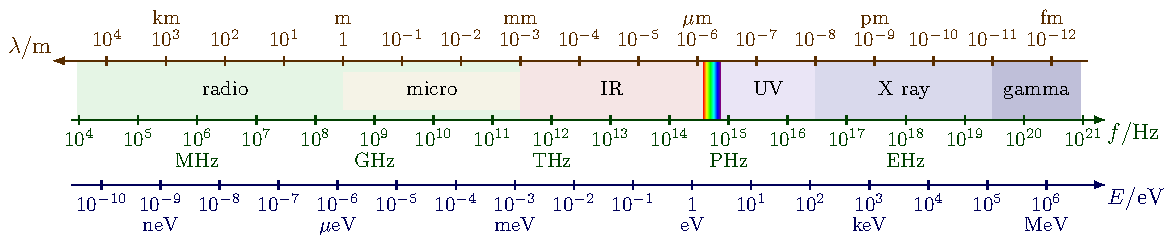
\includegraphics[width=\textwidth]{../images/em-spectrum/em-spectrum.pdf}
    \caption{\ref{source:em-spectrum} The electromagnetic spectrum.}
    \label{fig:em-spectrum}
\end{figure}
\begin{itemize}
    \item A \emph{progressive} wave is a wave in which \emph{energy is carried} from one point to another by means of \emph{vibrations or oscillations} within the wave. Particles within the wave are \emph{not transported along} the wave.
    \item A \emph{phase} is an angle which gives a measure of the \emph{fraction of a cycle} that has been \emph{completed} by an oscillating particle or by a wave.
    \item \emph{Intensity} of a wave is the wave energy incident per unit time per unit area \emph{normal} to the wave.
    \item \emph{Polarisation} of a wave refers to the \emph{confinement} of oscillations in \emph{only} one plane. The plane of oscillations is \emph{parallel} to the direction of energy transfer.  
\end{itemize}
\begin{minipage}{3cm+15.2363pt}
    \includegraphics[page=4]{../images/Malus'-Law/Malus'-Law.pdf}
\end{minipage}%
\begin{minipage}{\textwidth-3cm-15.2363pt}
    \begin{itemize}
        \item Malus' Law states that the intensity of a beam of \emph{plane polarised light} after passing through a rotatable polariser is directly proportional to the square of the cosine of the angle through which the polariser is rotated from the position that gives maximum intensity. (\(I=I_{\text{max}}\cos^2(\theta)\))
    \end{itemize}
\end{minipage}
    \begin{figure}[H]
        \centering
        \includegraphics[width=\textwidth,page=3]{../images/Malus'-Law/Malus'-Law.pdf}
        \caption{\ref{source:malus-law} An illustration of Malus' Law.}
        \label{fig:malus-law}
    \end{figure}
\begin{itemize}[label=\(\square\)]
    \item \begin{tabular}{|Sc|Sc|Sc|}
        \hline
        Phase Difference \(\Delta \phi\) & \(\frac{2\pi}{\lambda}\Delta x\) & \(\frac{2\pi}{T}\Delta t\)\\
        \hline
    \end{tabular}
    \item \begin{tabular}{|Sc|Sc|Sc|Sc|}
            \hline
            \multicolumn{4}{|Sc|}{Intensity}\\
            \hline
            \multirow{2}{*}{Amplitude} & \multicolumn{3}{Sc|}{Wave}\\
            \cline{2-4}
            & Spherical & Circular & Plane\\
            \hline
            \(I \propto A^2\) & \(I \propto \frac{1}{r^2}\) & \(I \propto \frac{1}{r}\) & \begin{minipage}{3cm}
                \vspace{1mm}\begin{center}
                    \(I\) is constant\\
                \tiny (No spreading of waves) \normalsize
                \end{center}
            \end{minipage}\\
            \hline
        \end{tabular}
        \item[\mbox{\FiveStarOpen}] When unpolarised light passes through a polariser, the average value of \(\cos^2(\theta)\) is \(\frac{1}{2}\) so \(I_\text{new}=\frac{1}{2}I_\text{max}\). 
\end{itemize}
\chapter{Superposition}
\begin{itemize}
    \item \emph{Principle of Superposition}: When two or more waves of the \emph{same type}, meet at \emph{a point in space}, the \emph{resultant displacement} of the waves at that point is the \emph{vector sum} of the \emph{displacements} due to \emph{each wave acting independently} at that point.
    \item \emph{Stationary waves} are waves whose \emph{waveforms do not advance} and there is \emph{no net translation of energy}. The \emph{amplitude} of the waves varies according to \emph{position} from zero at the nodes to a maximum at the antinodes.
    \item A stationary wave is formed when two \emph{progressive} waves
    \begin{enumerate}
        \item Having the \emph{same frequency} and \emph{same speed}
        \item Travel in \emph{opposite directions} towards each other
        \item Have \emph{similar amplitudes}
        \item Are unpolarised, or polarised along the same axis
        \item Are \emph{superposed} 
    \end{enumerate}
    \item \begin{tabular}{|Sc|Sc|Sc|}
        \hline
        \multirow{2}{*}{Properties} & \multicolumn{2}{Sc|}{Reflection Surface}\\
        \cline{2-3}
        & Loose End\footnotemark[1] & Fixed End\\
        \hline
        Allows for Oscillations? & Yes & No\\
        \hline
        Will Reflected Wave be Inverted (phase change of \(\pi\))? & No & Yes\\ 
        \hline
    \end{tabular}
    \footnotetext[1]{Particles of the wave can move about freely.}
    \item Characteristics of Stationary Waves:
    \begin{enumerate}
        \item Displacement node = Pressure antinode
        \item Displacement antinode = Pressure node
    \end{enumerate}
    \begin{longtable}{|Sc|Sc|Sc|}
        \hline
        Properties & Stationary Wave & Progressive Wave\\
        \hline
        Energy & No net transfer of energy & 
        \begin{minipage}{0.4\textwidth}
            Energy is transferred in the direction of propagation of the wave. 
        \end{minipage}\\
        \hline
        Phase & 
        \begin{minipage}{0.4\textwidth}
            \begin{itemize}[label=\(\square\)]
                \item Adjacent nodes: In phase
                \item Adjacent segments: Antiphase. \hyperlink{StationaryWavesPhase}{(Fig 12.1)}
            \end{itemize}
        \end{minipage} & 
        \begin{minipage}{0.4\textwidth}
            All points within one wavelength have different phases.
        \end{minipage}\\
        \hline
        Amplitude &
        \begin{minipage}{0.4\textwidth}
            Varies: 0 at nodes to max at antinodes.
        \end{minipage}
        &
        \begin{minipage}{0.4\textwidth}
            Same for all particles.
        \end{minipage}\\
        \hline
        Wavelength &
        \begin{minipage}{0.4\textwidth}
            Twice the distances between adjacent nodes or adjacent antinodes.
        \end{minipage} &
        \begin{minipage}{0.4\textwidth}
            Distance between adjacent in-phase particles. 
        \end{minipage}\\
        \hline
        Frequency &
        \multicolumn{2}{Sc|}{Same for all particles}\\
        \hline
        Nodes\footnotemark[2]/Antinodes\footnotemark[3] & \checkmark & \(\times\)\\
        \hline
    \end{longtable}
    \footnotetext[2]{At which particles don't oscillate/\(\text{amplitude}=0\).}
    \footnotetext[3]{At which particles have the largest amplitude.}
    \newpage
    \begin{center} \hypertarget{StationaryWavesPhase}{}
        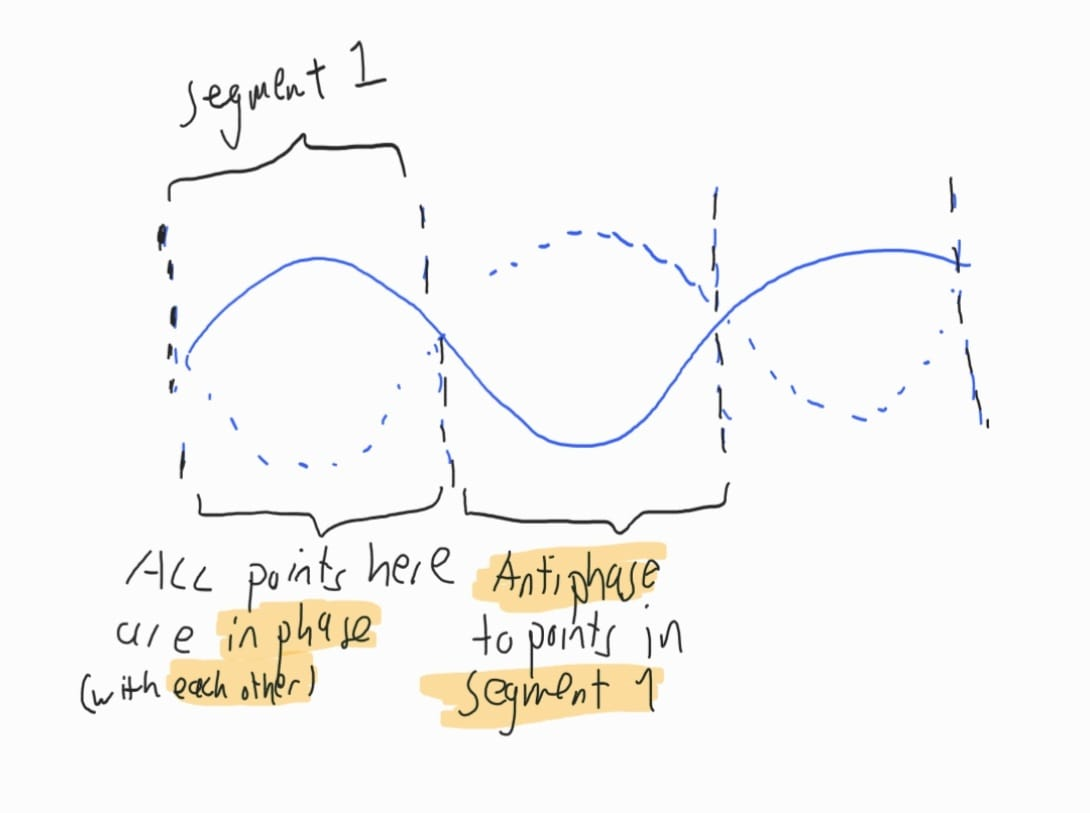
\includegraphics[scale=0.2]{../images/StationaryWavesPhase.jpg}
        \captionsetup{type=figure}
        \captionof{figure}{\ref{Me} Phases in stationary waves}
    \end{center}
    \resizebox{\textwidth}{!}{\begin{tabular}{|Sc|Sc|Sc|Sc|Sc|Sc|}
        \hline
        & \multicolumn{2}{Sc|}{Modes} & \multirow{2}{*}{Diagrams} & \multirow{2}{*}{Wavelength} & \multirow{2}{*}{Frequency}\\
        \cline{2-3}
        & Overtone & Harmonic &&&\\
        \hline
        Strings/Open Pipes & \multirow{2}{*}{\(n\)th} & \((n+1)\)th & \hyperlink{Fig 12.2}{12.2} \& \hyperlink{Fig 12.3}{12.3} & \(\lambda=\frac{2L}{n+1}\) & \(f=(n+1)\frac{v}{2L}\)\\
        \cline{1-1}
        \cline{3-6}
        Pipes Closed at One End & & \((2n+1)\)th & \hyperlink{Fig 12.4}{12.4} \& \hyperlink{Fig 12.5}{12.5} & \(\lambda=\frac{4L}{2n+1}\) & \(f=(2n+1)\frac{v}{4L}\)\\
        \hline
    \end{tabular}}
    \begin{minipage}{0.3\textwidth}
        \begin{center}
            \hypertarget{Fig 12.2}{}
            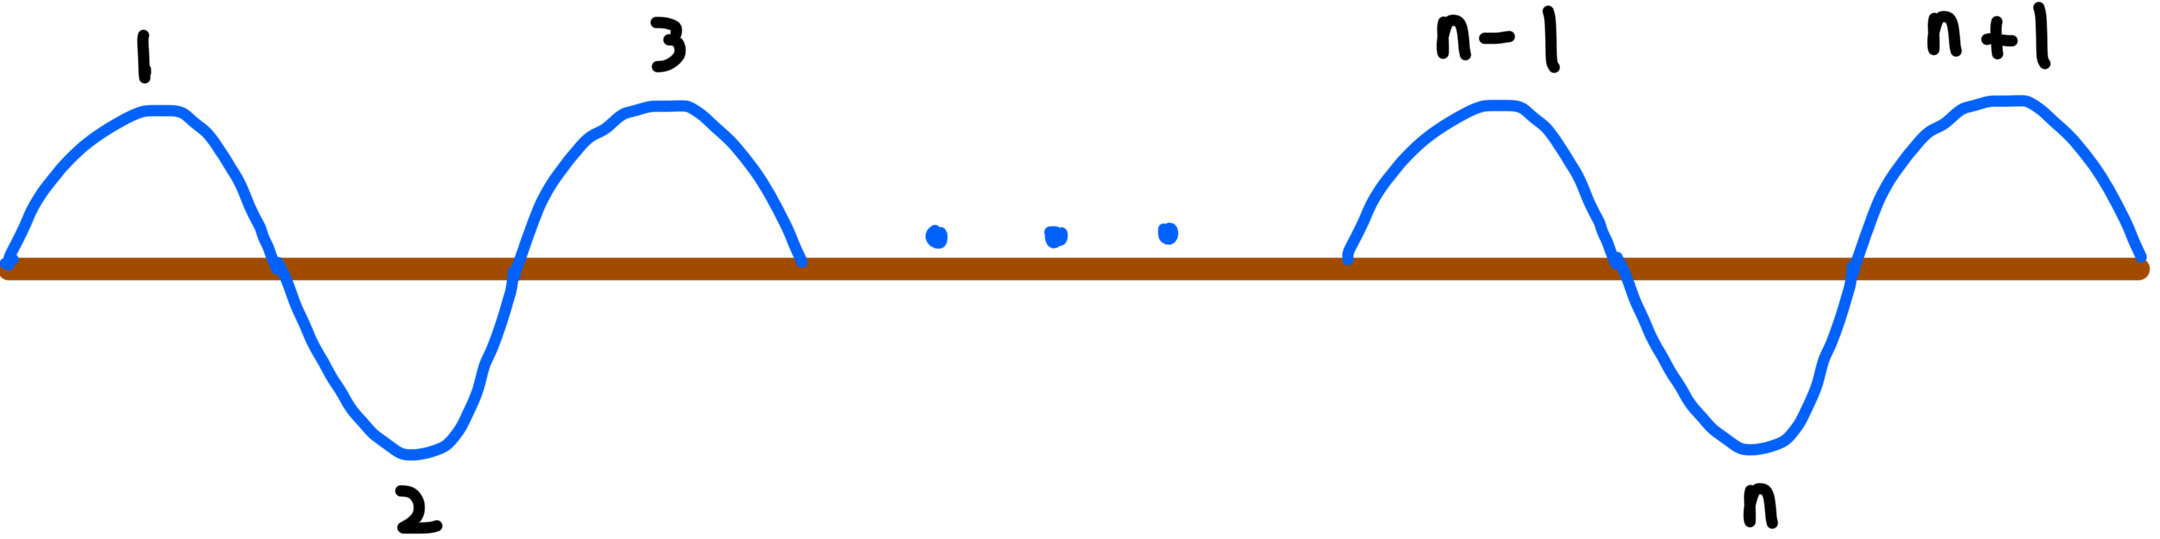
\includegraphics[scale=0.1]{../images/StringStatWaves.jpg}
            \captionsetup{type=figure}
            \captionof{figure}{\ref{RVHS} String.}
        \end{center}
    \end{minipage}
    \begin{minipage}{0.3\textwidth}
        \begin{center}
            \hypertarget{Fig 12.3}{}
            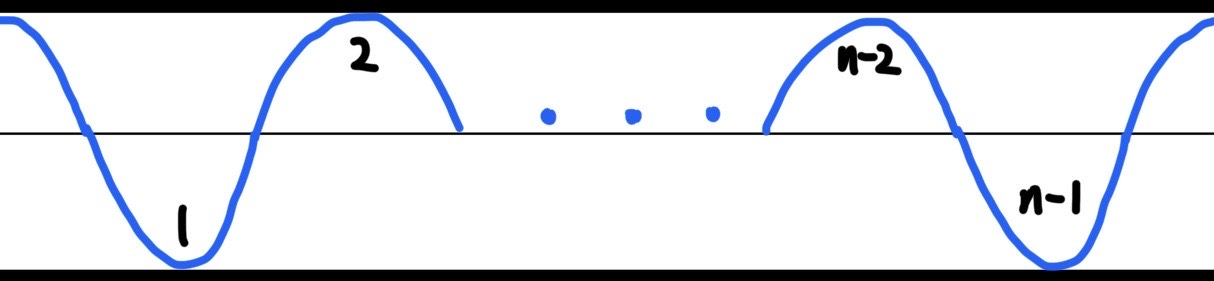
\includegraphics[scale=0.1]{../images/Open Pipe.jpg}
            \captionsetup{type=figure}
            \captionof{figure}{\ref{RVHS} Open pipe.}
        \end{center}
    \end{minipage}
    \begin{minipage}{0.3\textwidth}
        \vspace{7mm}
        \begin{center}
            \hypertarget{Fig 12.4}{}
            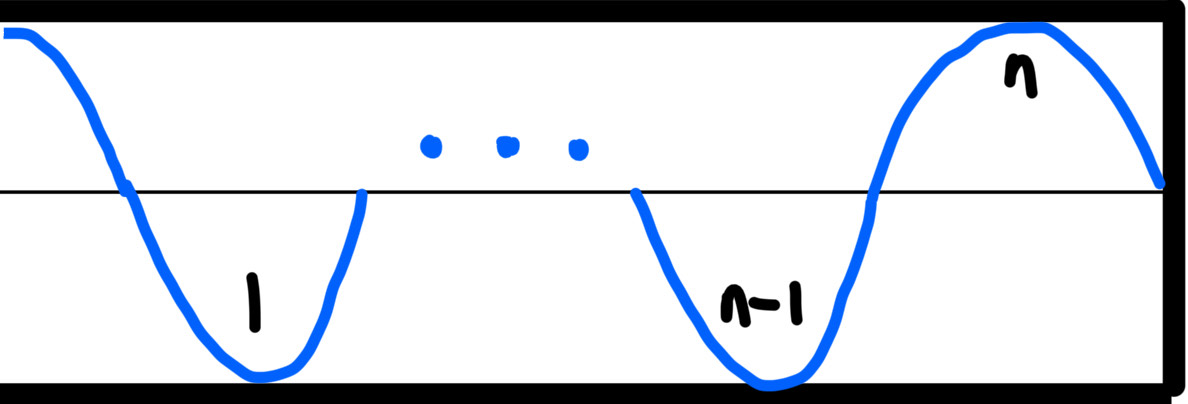
\includegraphics[scale=0.1]{../images/Pipe Closed at One End.jpg}
            \captionsetup{type=figure}
            \captionof{figure}{\ref{RVHS} Pipe closed at one end}
        \end{center}
    \end{minipage}
    \begin{center}
        \hypertarget{Fig 12.5}{}
        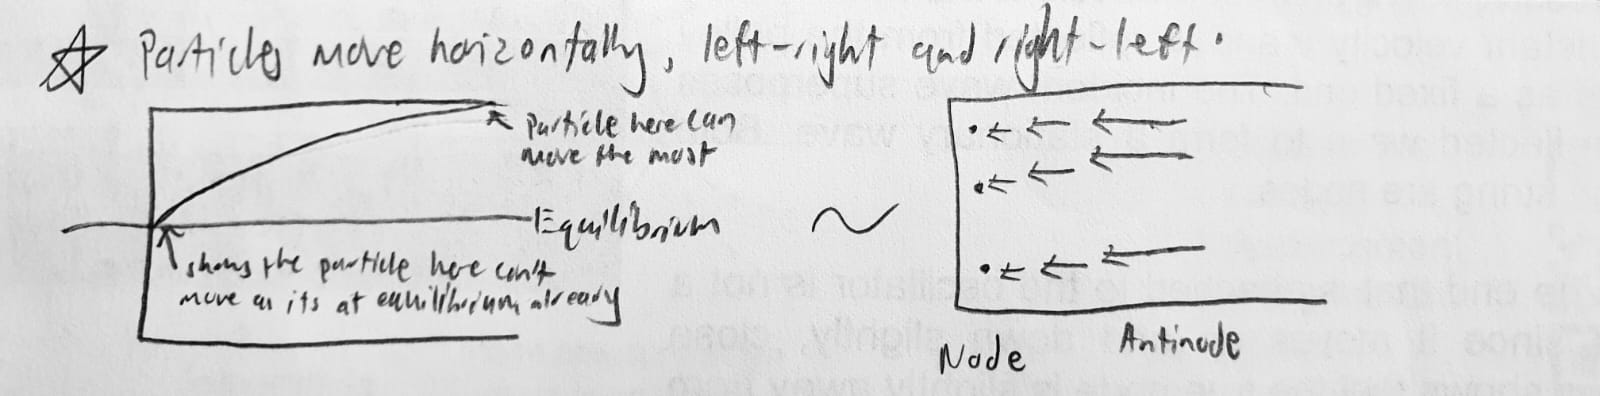
\includegraphics[scale=0.25]{../images/Pipe Closed At One End Movement.jpg}
        \captionsetup{type=figure}
        \captionof{figure}{Movement of particles in pipe.}
    \end{center}
    \setcounter{footnote}{1}
    \item Resonance length\footnote{End correction: Actual length of vibration is \(L+2c\) for open pipes, and \(L+c\) for closed pipes.} with pipes closed at one end 
    \[L=\frac{\lambda}{4}=\frac{v}{4f}.\]
    \begin{example}{}{}
        Explain, with reference to resonance, why the loudness of sound changes as the water level changes.
        \begin{enumerate}
            \item Natural frequency of vibration depends on length of air column.
            \item When fork frequency is equal to natural frequency/odd multiple of fundamental frequency, resonance occurs. There is maximum energy transfer and maximum amplitude of vibrations, leading to maximum loudness.
            \item When fork frequency is not equal to natural frequency, no resonance occurs and loudness drops.
        \end{enumerate}
    \end{example}
    \item If a tube achieves stationary waves at fundamental frequency \(f\), then reducing \(f\)/increasing \(\lambda\) will not result in stationary waves.
    \item \emph{Diffraction} is the \emph{bending or spreading out} of waves when they travel through a \emph{small opening} or when they pass round a \emph{small obstacle}.
    \item Large amount of diffraction occurs when the width of slit is about the same as the wavelength.
    \item The wavelength before and after diffraction should be around the same.
    \item Single Slit Diffraction: Let \(b\) be the slit width, and \(L\) the slit-screen distance.
    \begin{enumerate}
        \item For all nonzero integers \(m\), the angular positions \(\theta\) of the \(1 \leq m\)th order minima satisfies 
        \[\sin(\theta)=\frac{m\lambda}{b}.\] 
        \item Distance \(y_1\) of the first minima from either side of the central bright fringe is
        \[y_1=\frac{\lambda L}{b}.\]
    \end{enumerate}
    \begin{center}
        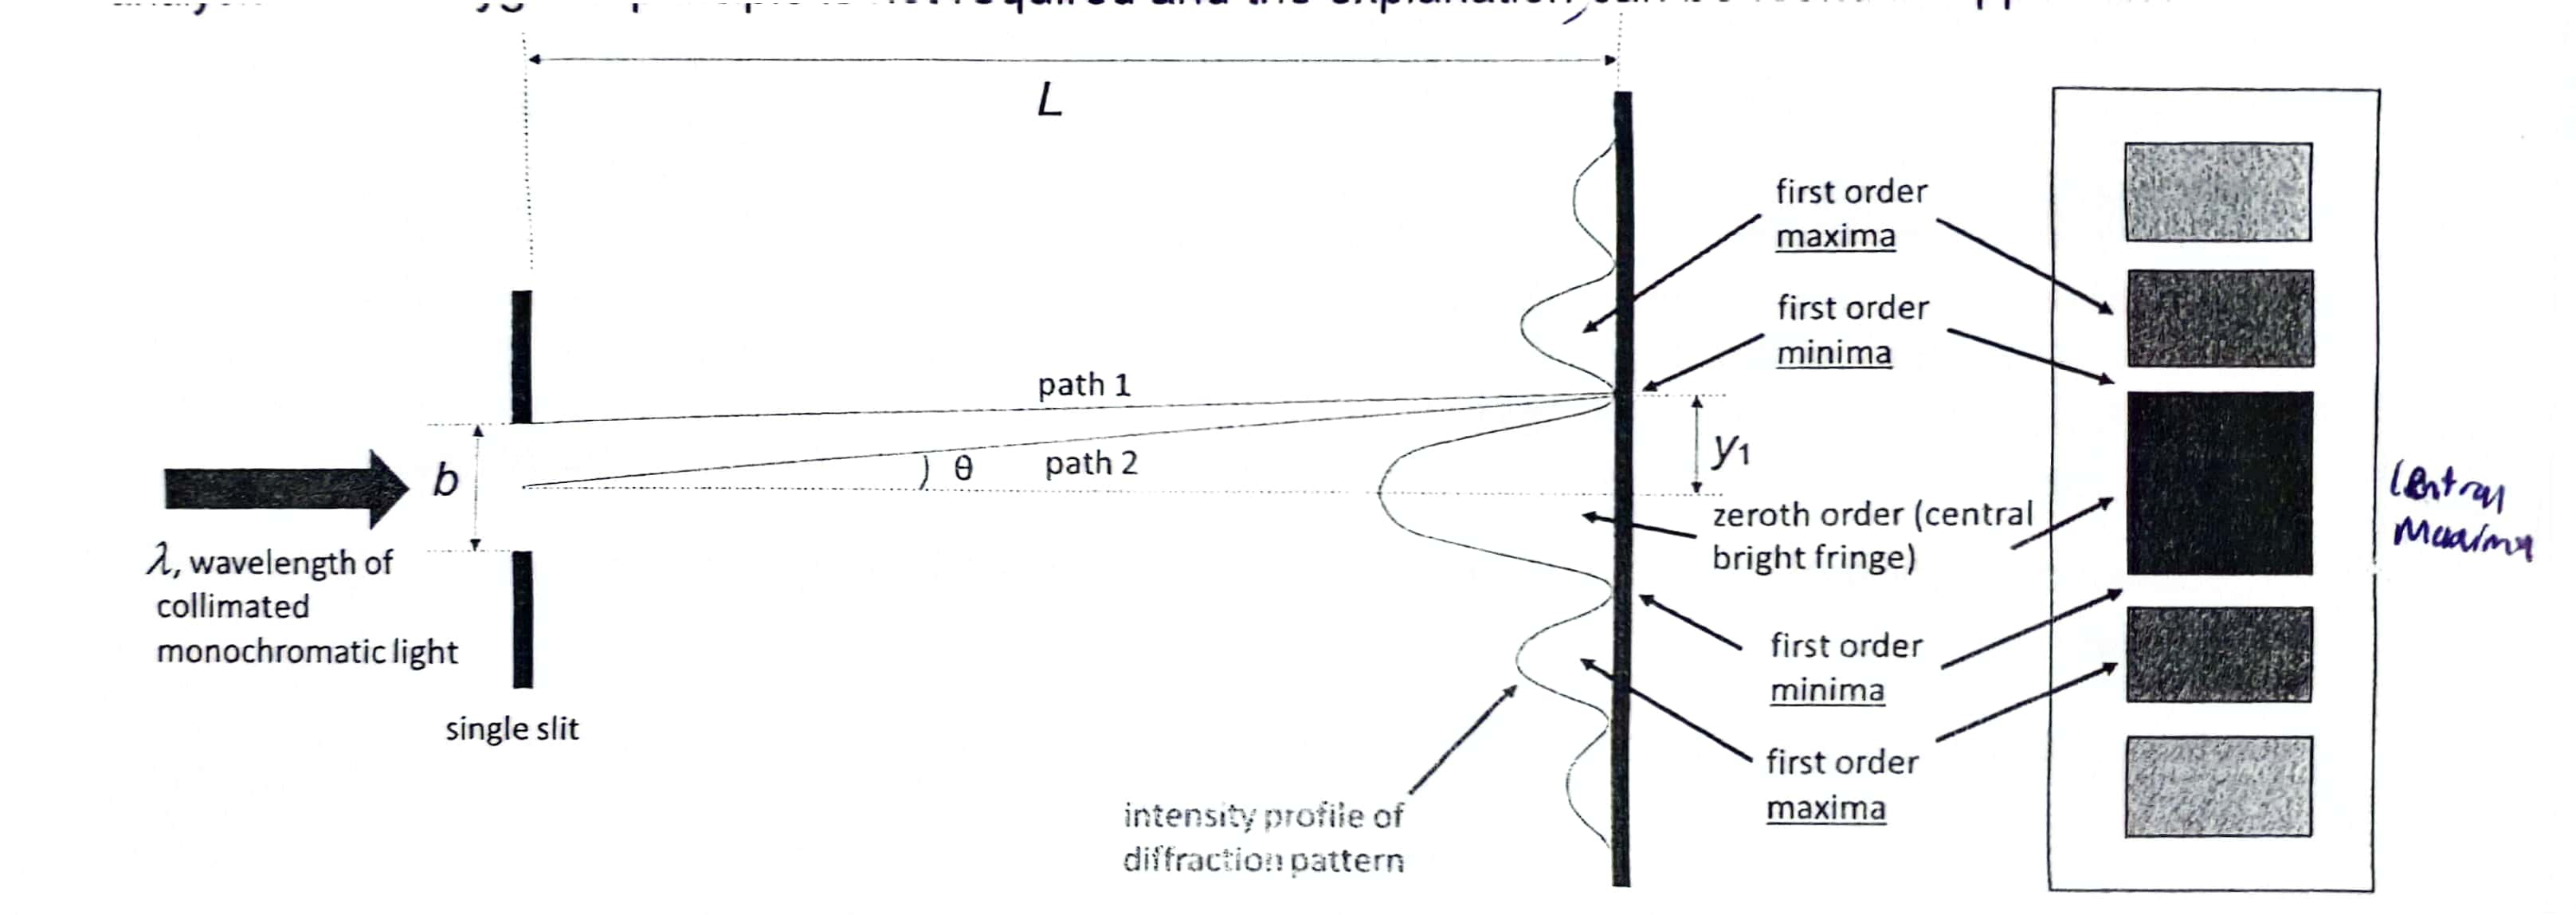
\includegraphics[scale=0.1]{../images/Single Slit Diffraction.jpg}
        \captionsetup{type=figure}
        \captionof{figure}{\ref{RVHS} Single slit diffraction.}
    \end{center}
    \item \emph{Circular} aperture: \(\theta \approx \frac{\lambda}{b}\).
    \item \emph{Rayleigh's Criterion} is the \emph{minimum separation} between two objects in order to be distinguished as two \emph{distinct} objects:
    \[\theta \approx \frac{\lambda}{b}.\]
    \item Sources are \emph{coherent} if they have a \emph{constant phase difference} with respect to time.
    \item \emph{Interference} is the \emph{superposing} of two or more waves to produce \emph{regions of maxima and minima} in space, according to the \emph{Principle of Superposition}.
    \item Conditions for an \emph{observable} interference pattern: 
    \begin{enumerate}
        \item The waves must \emph{overlap} to produce regions of maxima and minima.
        \item The \emph{sources} must be \emph{coherent}.
        \item The waves must have approximately the \emph{same amplitude}.
        \item The waves, if transverse, must be \emph{unpolarised} or have the \emph{same plane of polarisation}. 
    \end{enumerate}
    \item For \(n \in \mathbb{Z}^{+}_{0}\), representing the \(n\)th order max/min, we have 
    \resizebox{\textwidth}{!}{\begin{tabular}{|Sc|Sc|Sc|}
        \hline
        \multirow{2}{*}{Sources' Phase Difference} & \multicolumn{2}{Sc|}{Path Difference}\\
        \cline{2-3}
         & Constructive Interference (maxima) & Destructive Interference (minima)\\
        \hline 
        In phase & \(\Delta=n\lambda\) & \(\Delta=(n+1/2)\lambda\)\\
        \hline
        Out-of-phase & \(\Delta=(n+1/2)\lambda\) & \(\Delta=n\lambda\)\\
        \hline
    \end{tabular}}
    \item We always need to take the path difference starting from the actual source itself, even when the source travels through two slits onto a screen, for instance.
    \item Double-slits: For\footnote{Typical values: \(a \approx 0.5\)mm, \(D \approx 1\)m, and \(\lambda \approx 600\)nm. In any case, using the equation requires \(a<<D\).} a (\emph{center-to-center}) slit separation \(a\) and slit-screen distance \(D\), the fringe separation (between two adjacent minima, or two adjacent maxima) is
    \[x=\frac{\lambda D}{a}.\]
    \begin{center}
        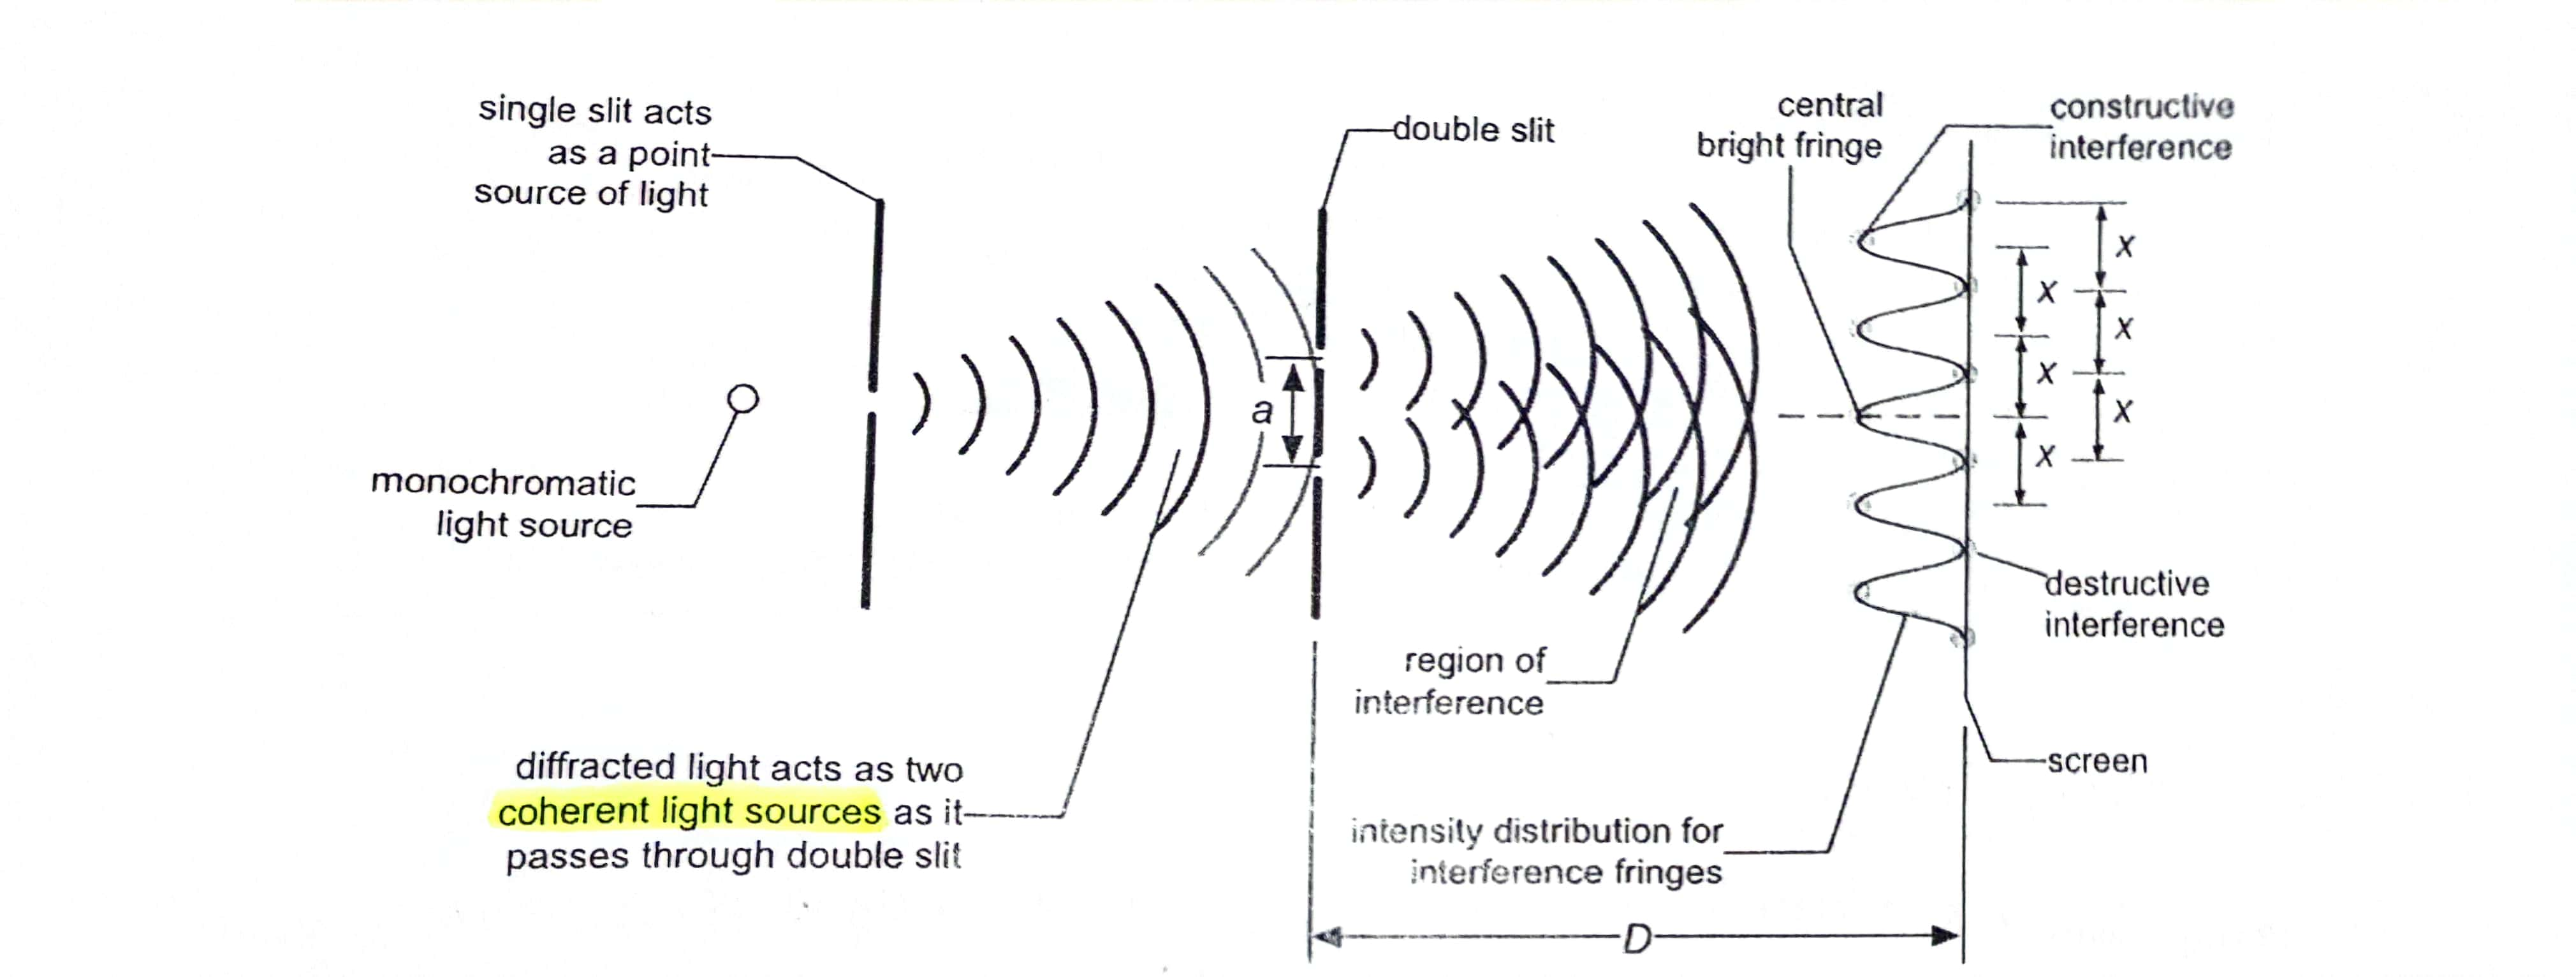
\includegraphics[scale=0.1]{../images/Double-Slit Diffraction.jpg}
        \captionsetup{type=figure}
        \captionof{figure}{\ref{RVHS} Double-slit diffraction.}
    \end{center}
    \setcounter{footnote}{4}
    \footnotetext{The intensity of the double-slit interference pattern is not constant because of single-slit diffraction effects.}
    \item Diffraction grating: For a slit-separation \(d\) and \(n \in \mathbb{Z}^{+}_{0}\), the angular positions for the \(n\)th order maxima satisfies
    \[d \sin(\theta_n)=n\lambda.\]
    \begin{center}
        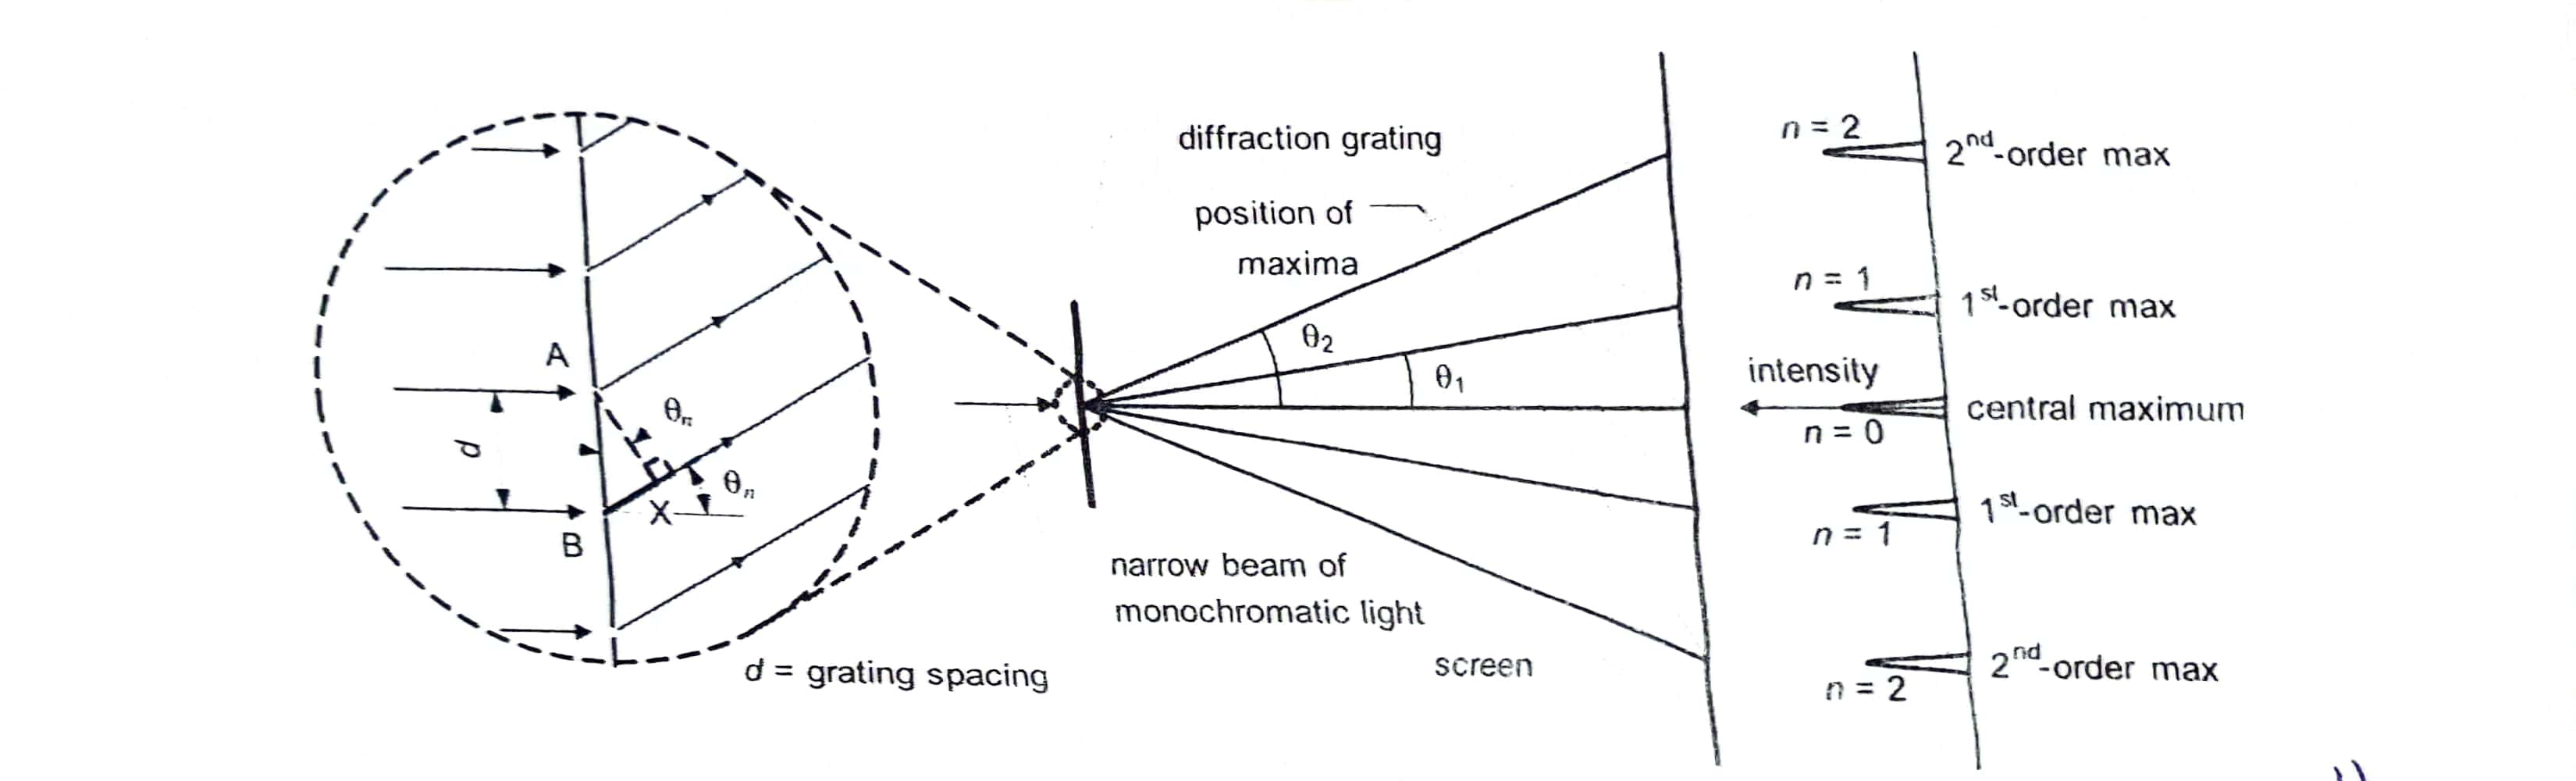
\includegraphics[scale=0.1]{../images/Diffraction Grating.jpg}
        \captionsetup{type=figure}
        \captionof{figure}{\ref{RVHS} Diffraction grating.}
    \end{center}
    \item Check answer: For visible light, \(400\text{nm} \leq \lambda \leq 700\text{nm}\).
    \item Total number of bright regions = 2\(\cdot\)highest order+1.
    \item When slit width is reduced, intensity is reduced.
    \item To calculate \emph{resultant intensity}, first take the sum of the amplitudes and use proportionality (\(I \propto A^2\)).  
    \item Every other line means half of the lines are covered.
    \begin{example}{}{}
        Describe and explain the appearance of the central fringe if the light is now replaced with white light.
    \begin{enumerate}
        \item The central bright fringe is generally white.
        \item The zeroth order fringes of all the wavelengths coincide at the center where the path difference from the two slits is zero for all wavelengths. The combined central fringes remains white.
        \item The sides of the central fringes are likely more reddish.
        \item  This is because the wider red fringe extends beyond the narrower blue fringe.
    \end{enumerate}
    \end{example}
\end{itemize}

\chapter{Currents of Electricity}
\begin{itemize}
    \item The \emph{number density} \(n\) is defined as the number of particles per unit volume.
    \item The \emph{drift velocity} \(v\) is the \emph{average} velocity at which \emph{charge carriers} move through a \emph{conductor} when there is \emph{electric current in the conductor}.
    \item Deriving the equation \(I=nAvq\):
    \begin{enumerate}
        \item Assume that the \emph{current is constant}. Then, \(I=\frac{Q}{t}\).
        \hspace*{0pt}\hfill \(\highlight[yellow]{[n]}\)
        \item Assume that there are \(N\) charge carriers passing through a cross-sectional area \(A\) in time \(t\), and that \emph{each} of them carries an \emph{identical amount of charge} \(q\). Then, the \emph{total charge} that passing through \(A\) in time \(t\) is
        \[Q=Nq \tag*{\(\highlight[yellow]{[N,A(t),Q(t)]}\)}.\]
        \item Assume that the \emph{number density} \(n\) of charge carriers is \emph{uniform}, and let \(V\) be the volume covered by the current in time \(t\). Thus,
        \[N=nV \tag*{\(\highlight[yellow]{[n,V(t)]}\)}.\]
        \item Furthermore, since the current travels at some velocity \(v\),
        \[V=A\Delta x=Avt \tag*{\(\highlight[yellow]{[v]}\)}.\]
        \item Therefore, 
        \[I=\frac{Q}{t}=\frac{Nq}{t}=\frac{nVq}{t}=\frac{nAvtq}{t}=nAvq.\]
    \end{enumerate}
    \item Elementary charge \(e=1.6\times 10^{-19}C\) (Charge of an electron/proton).
    \item The \emph{potential difference} between \emph{two points} of a circuit is defined as the amount of electrical energy \emph{converted} to other forms of energy \emph{per unit charge} moved \emph{between} the two points. 
    \item \emph{Ohm's Law} states that the \emph{current} flowing in a \emph{conductor} is \emph{directly proportional} to the \emph{potential difference across it} under \emph{constant physical conditions}.
    \item \emph{Resistance} is defined as the \emph{ratio} of the \emph{potential difference across} the conductor to the \emph{current} flowing through it.
    \item \emph{Resistivity} \(\rho\) is the \emph{proportionality constant} between the \emph{dimensions of a specimen of a material} and its \emph{resistance} such that 
    \[R=\frac{\rho L}{A}.\]
    \newpage
    \item Electrical Components
    \begin{longtable}{|Sc|Sc|Sc|}
        \hline
        Types of Conductors & Changes to Resistance & Reason\\
        \hline
        \begin{minipage}{0.25\textwidth}
            Metallic conductor at constant temperature
        \end{minipage} &  
        \begin{minipage}{0.3\textwidth}
            \begin{itemize}
                \item At \emph{ constant temperature} this is an Ohmic conductor.
                \item Has \emph{constant resistance}. Ratios of \(V/I\) is constant.
            \end{itemize} 
            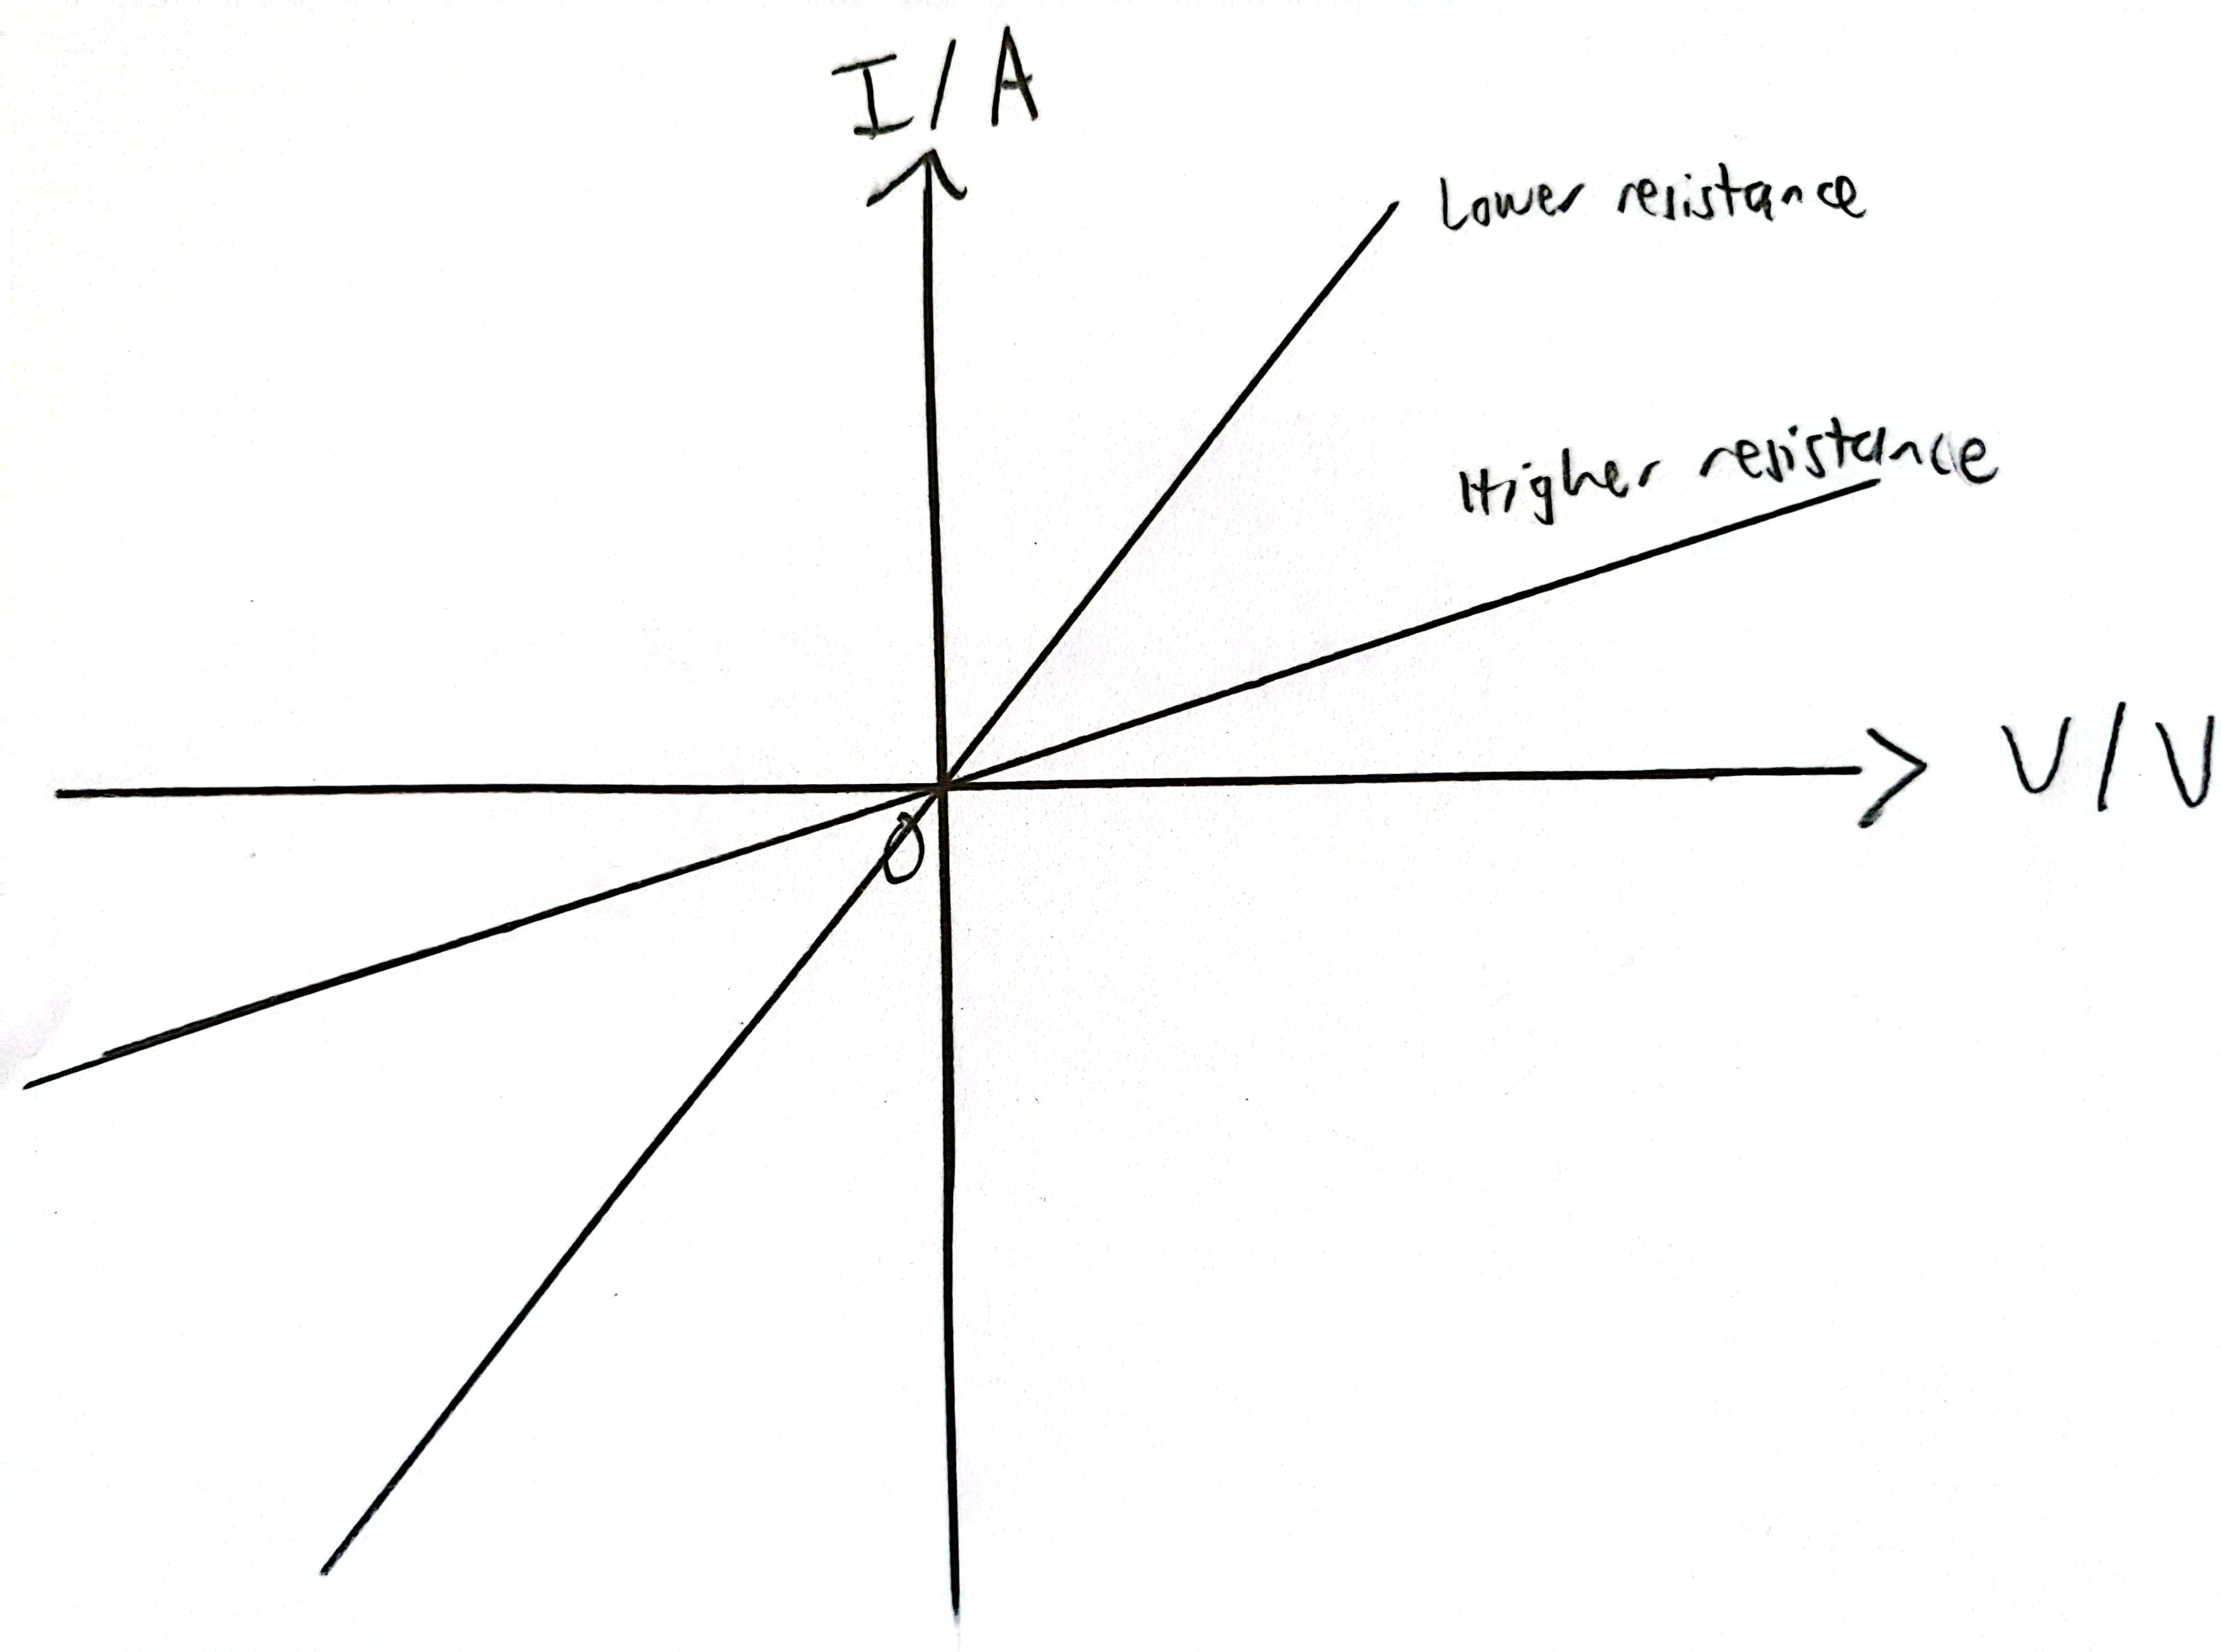
\includegraphics[width=\textwidth]{../images/MetallicConductor I-V.jpg}
        \end{minipage} &
        \begin{minipage}{0.3\textwidth}
            \begin{itemize}
                \item At \emph{constant temperature}, the \emph{number of free electrons} and the \emph{rate of atomic vibration} is constant.
                \item A resistor at a different constant temperature will have a difference resistance, and hence, \(V/I\) ratio. 
            \end{itemize}
        \end{minipage}\\
        \hline
        \begin{minipage}{0.25\textwidth}
            Semiconductor Diode\\[5mm]
            \begin{center}
                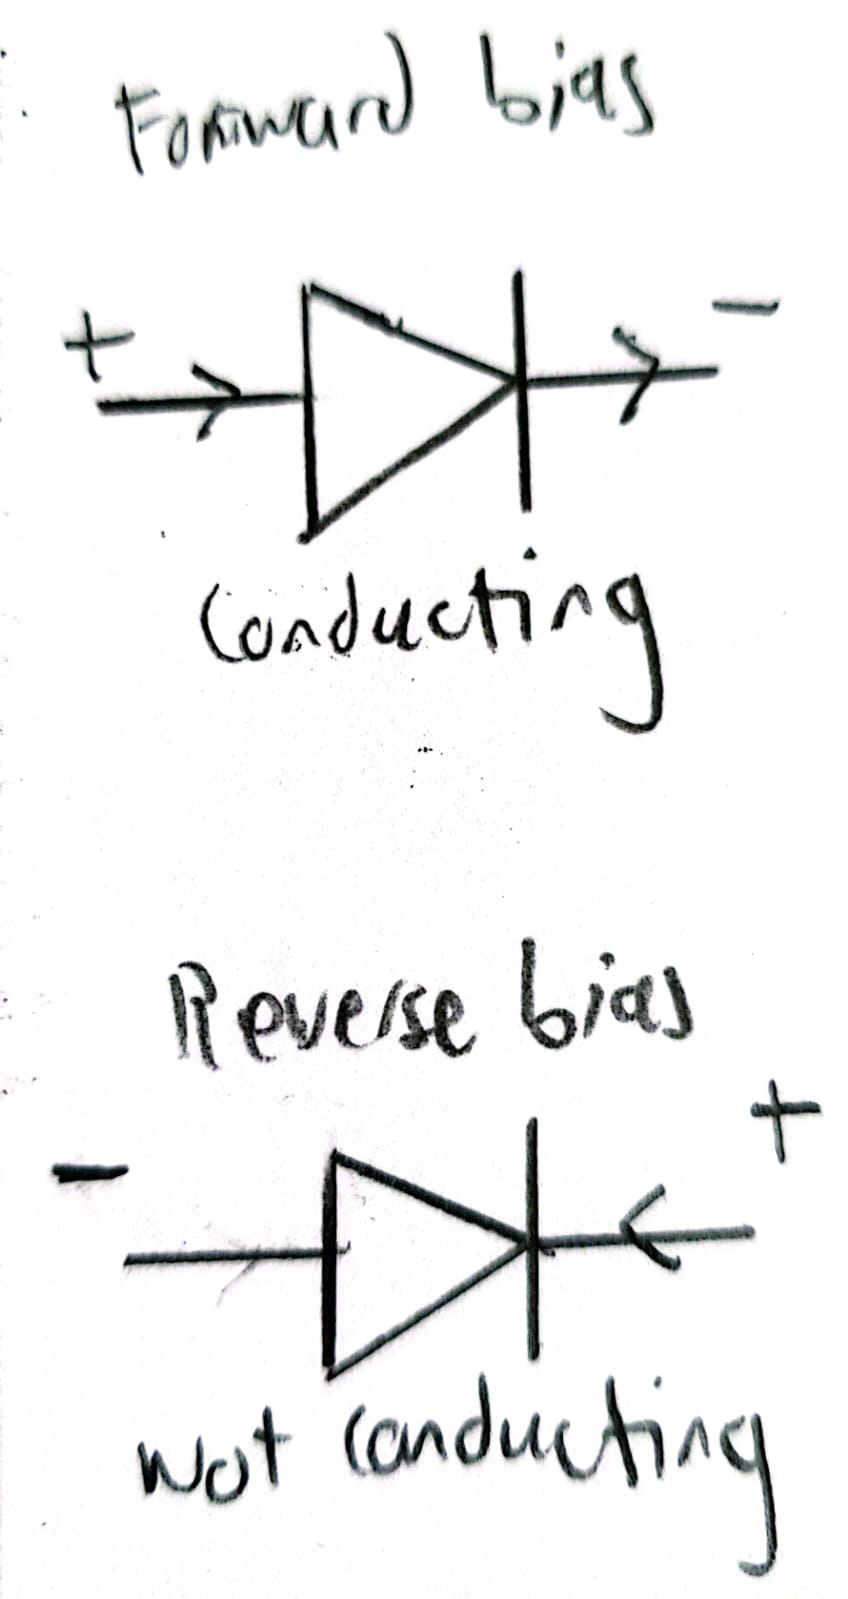
\includegraphics[scale=0.08]{../images/ForwardReverseBias.jpg}
            \end{center}
        \end{minipage} &
        \begin{minipage}{0.3\textwidth}
            \begin{itemize}
                    \item Forward-biased: \emph{Resistance decreases} when \emph{p.d. increases}. In fact, if the forward-biased p.d. goes past its \emph{threshold voltage}, \emph{resistance} becomes very low.
                    \item Reverse-biased: \emph{Very high resistance}. But, there will be a \emph{small leakage current}.
                    \item If the reverse-biased p.d. is so high that it exceeds the \emph{breakdown voltage}, the diode will \emph{break down} and \emph{conduct electricity}.
            \end{itemize} 
            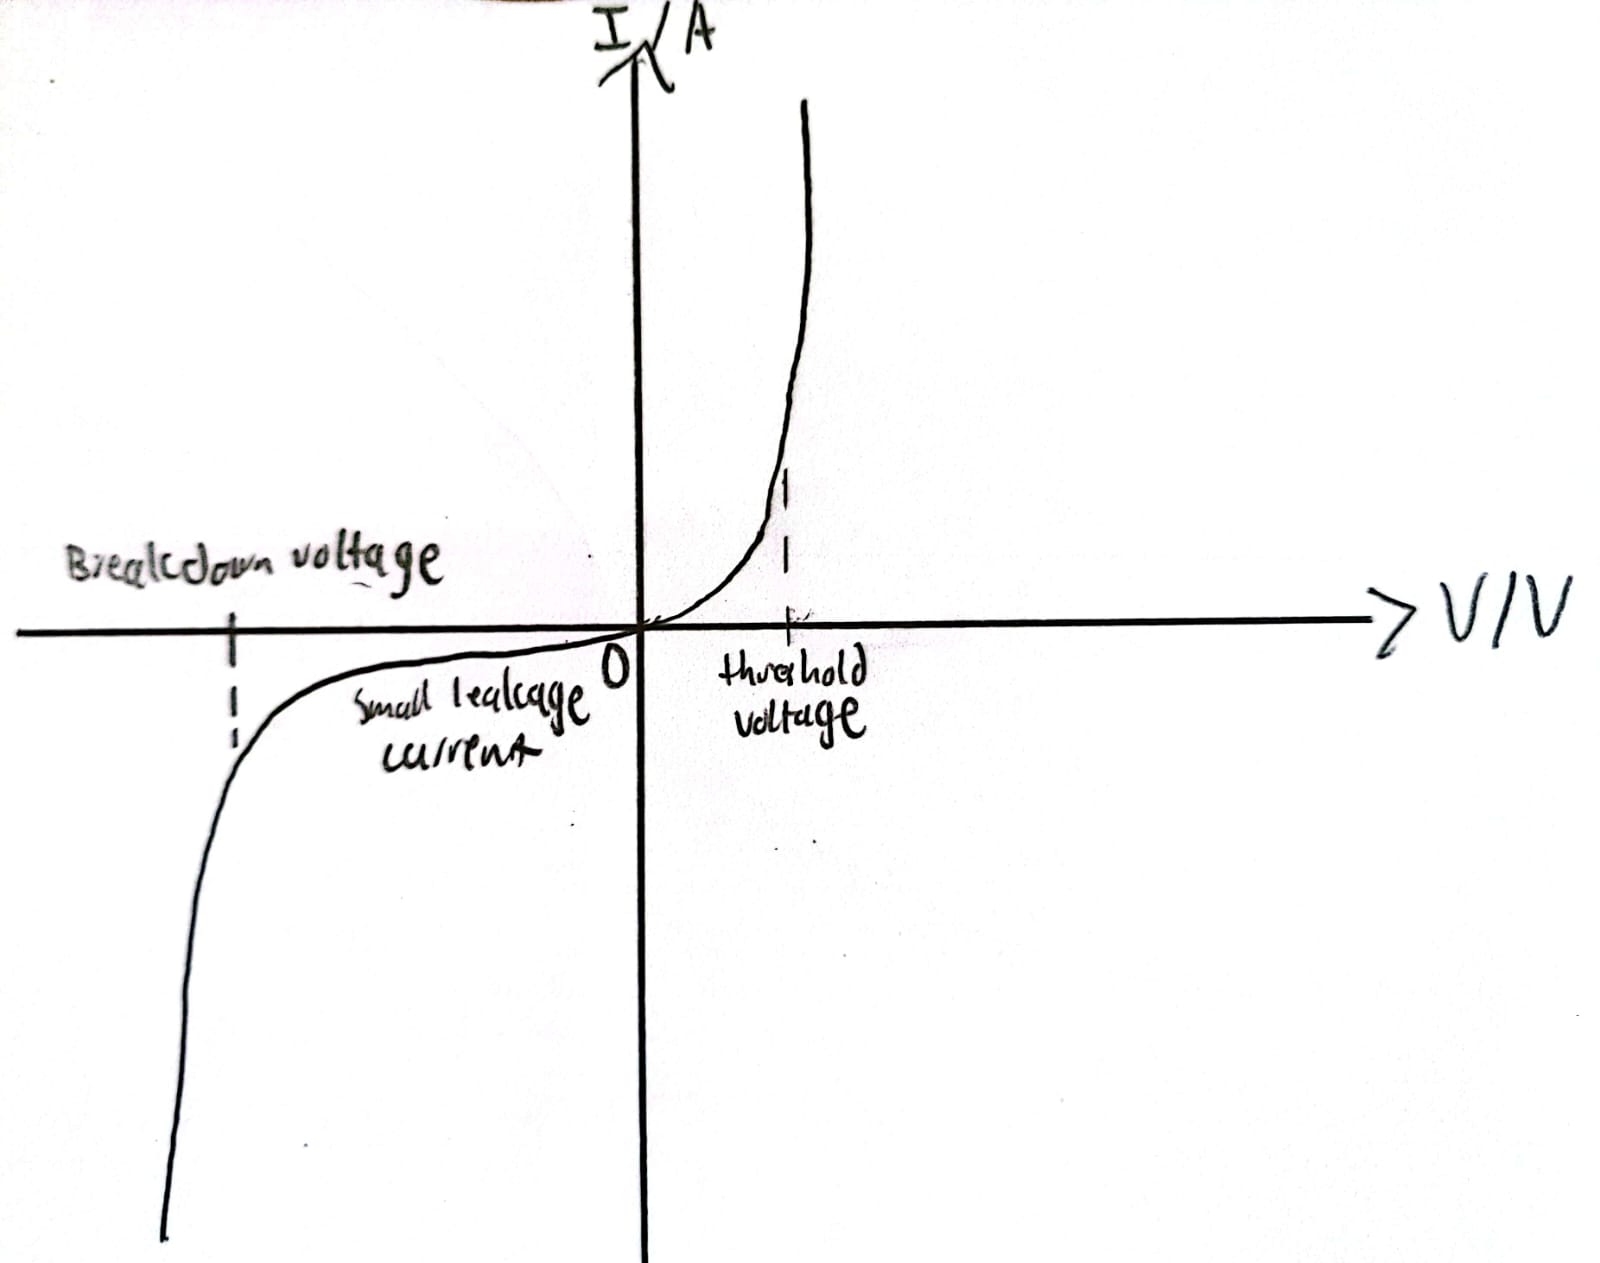
\includegraphics[width=\textwidth]{../images/Diode I-V characteristics.jpg}
        \end{minipage} &
        \begin{minipage}{0.3\textwidth}
            \begin{itemize}
                \item When connected in \emph{forward bias}, the circuit's \emph{electric field set up} allows for available \emph{charge carriers to flow} through, allowing it to conduct with \emph{low resistance}.
                \item When connected in \emph{reverse bias}, the circuit's electric field set up creates a \emph{widened `depletion region'} in the diode which \emph{impedes charge carriers} from flowing through the region, creating a \emph{large resistance}. 
            \end{itemize}
        \end{minipage}\\
        \hline
        \begin{minipage}{0.25\textwidth}
            Filament Lamp
        \end{minipage} &  
        \begin{minipage}{0.3\textwidth}
            \begin{itemize}
                \item When \emph{p.d. increases, current increases}, with \emph{decreasing \(I\)-\(V\) ratio}.
                \item The \emph{resistance} of a metallic conductor \emph{increases} with an increase in \emph{temperature}.
            \end{itemize} 
            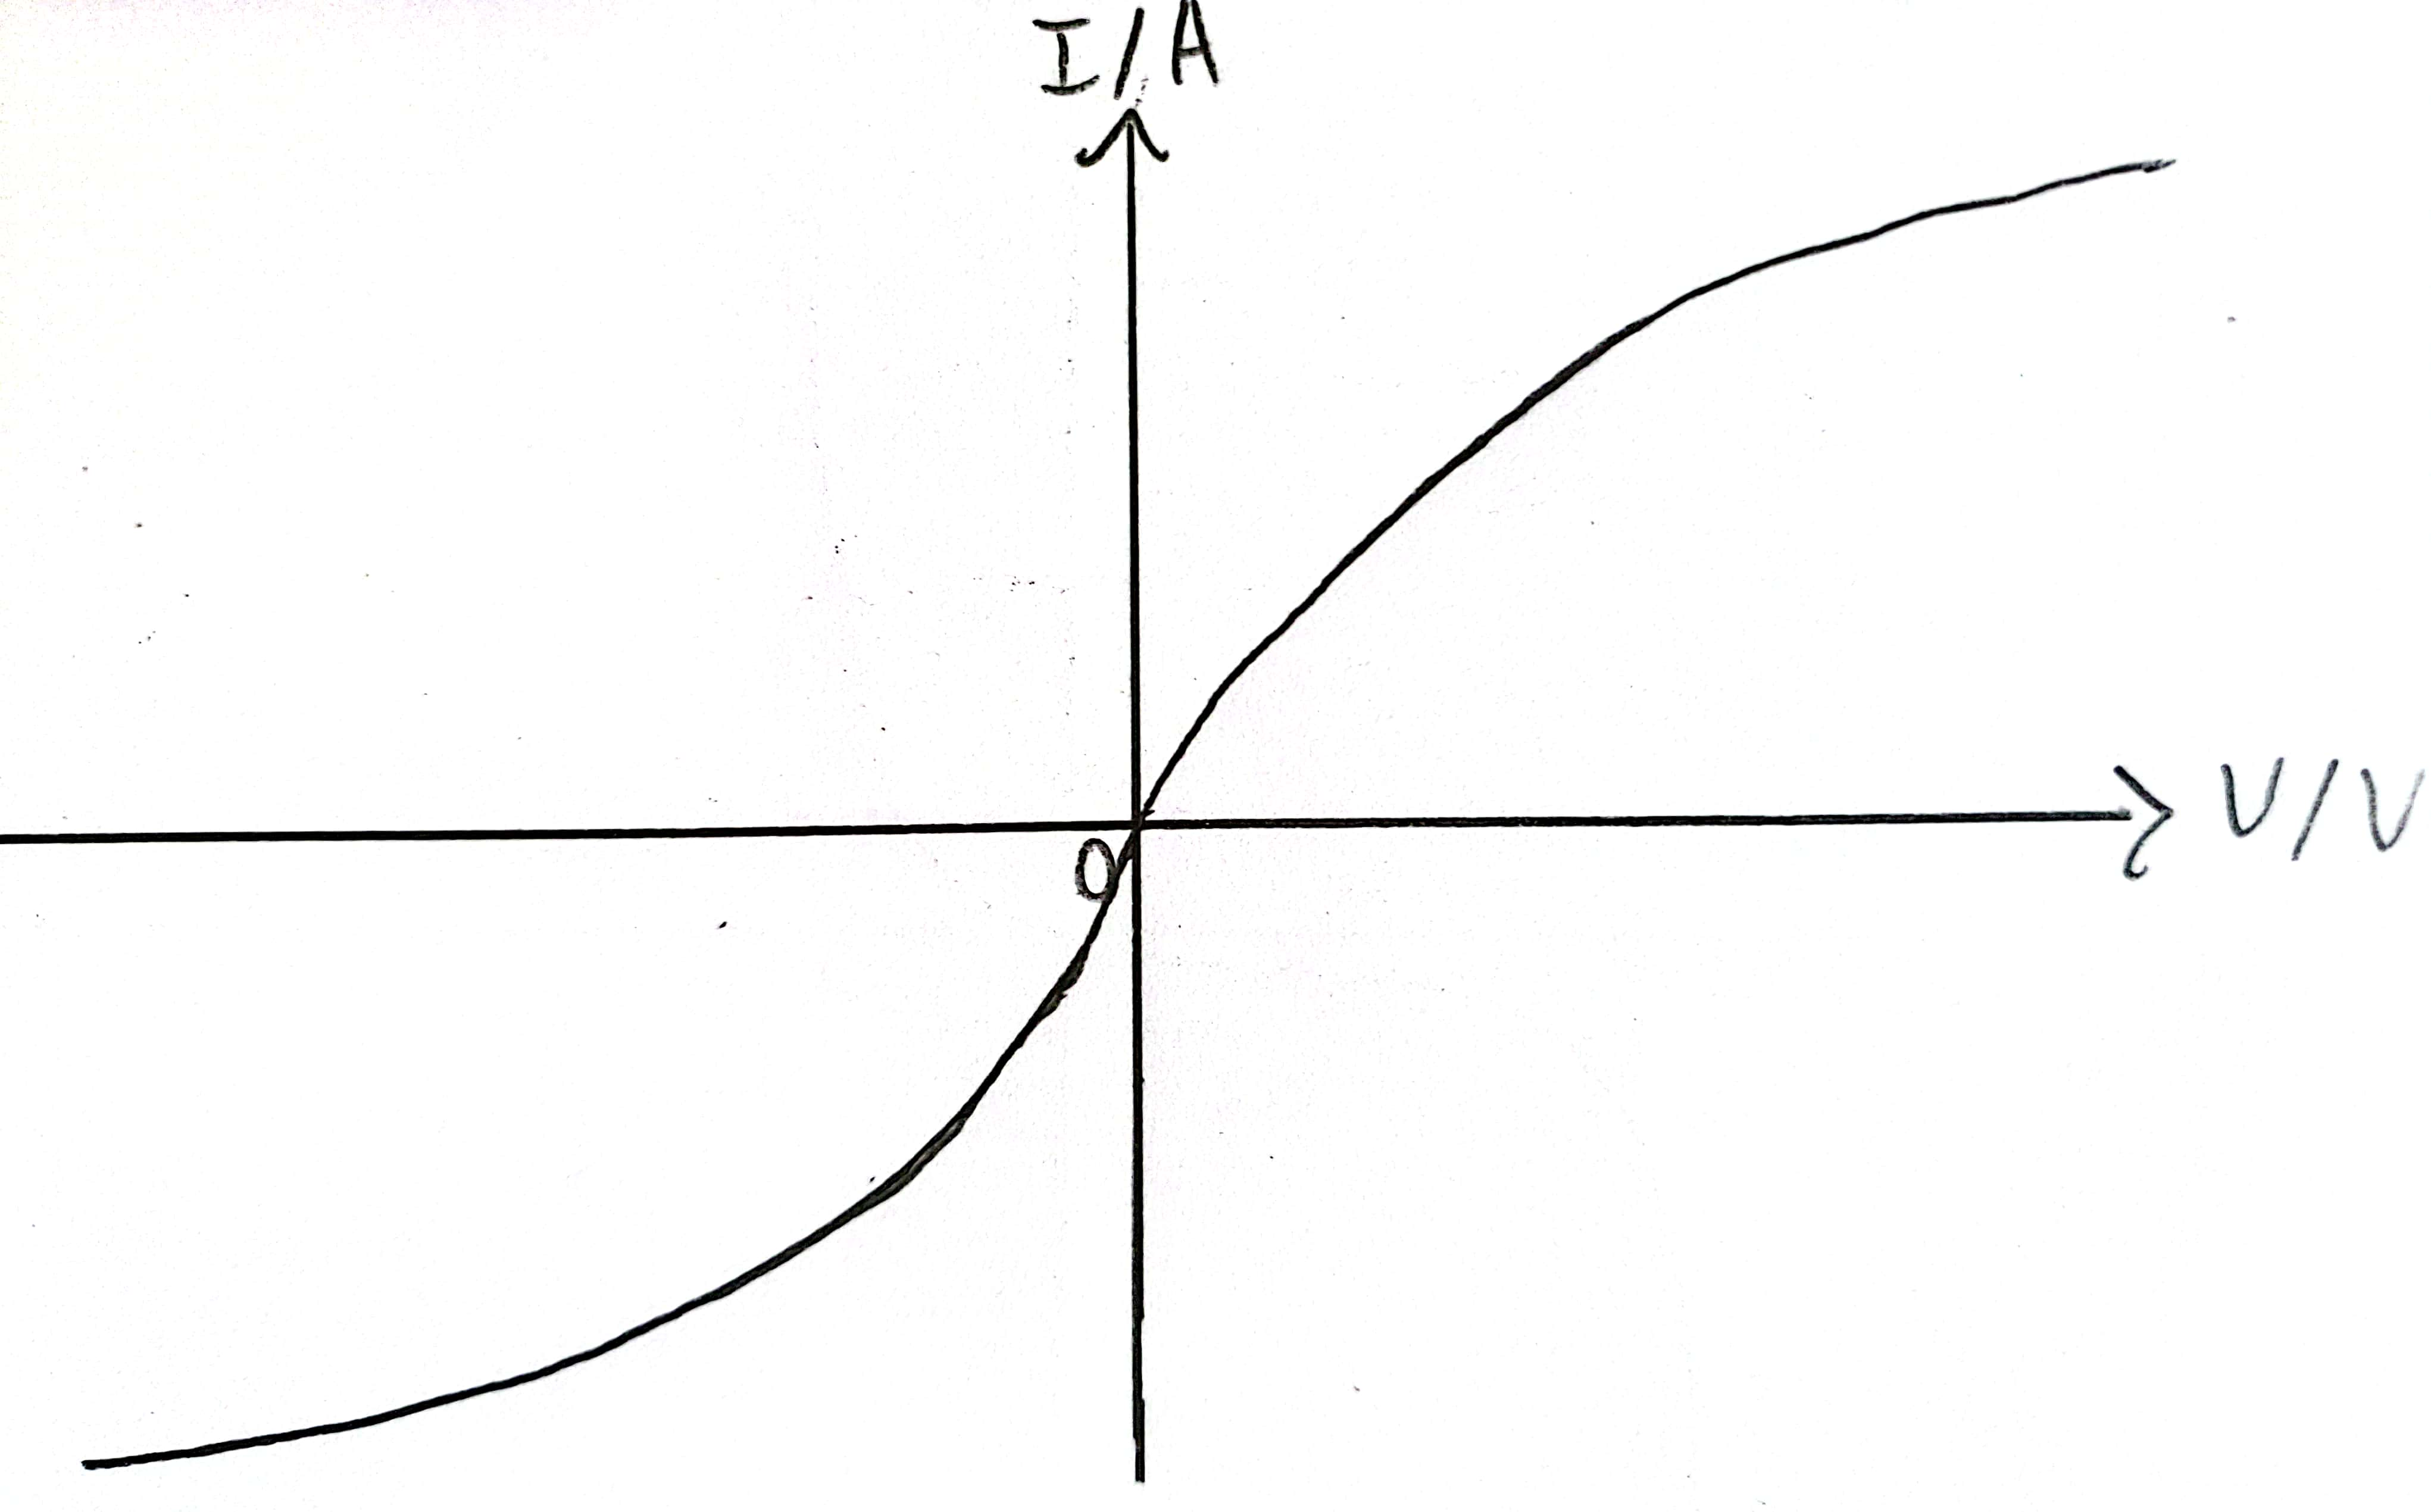
\includegraphics[width=\textwidth]{../images/Filament Lamp I-V Characteristics.jpg}\\[-1mm]
            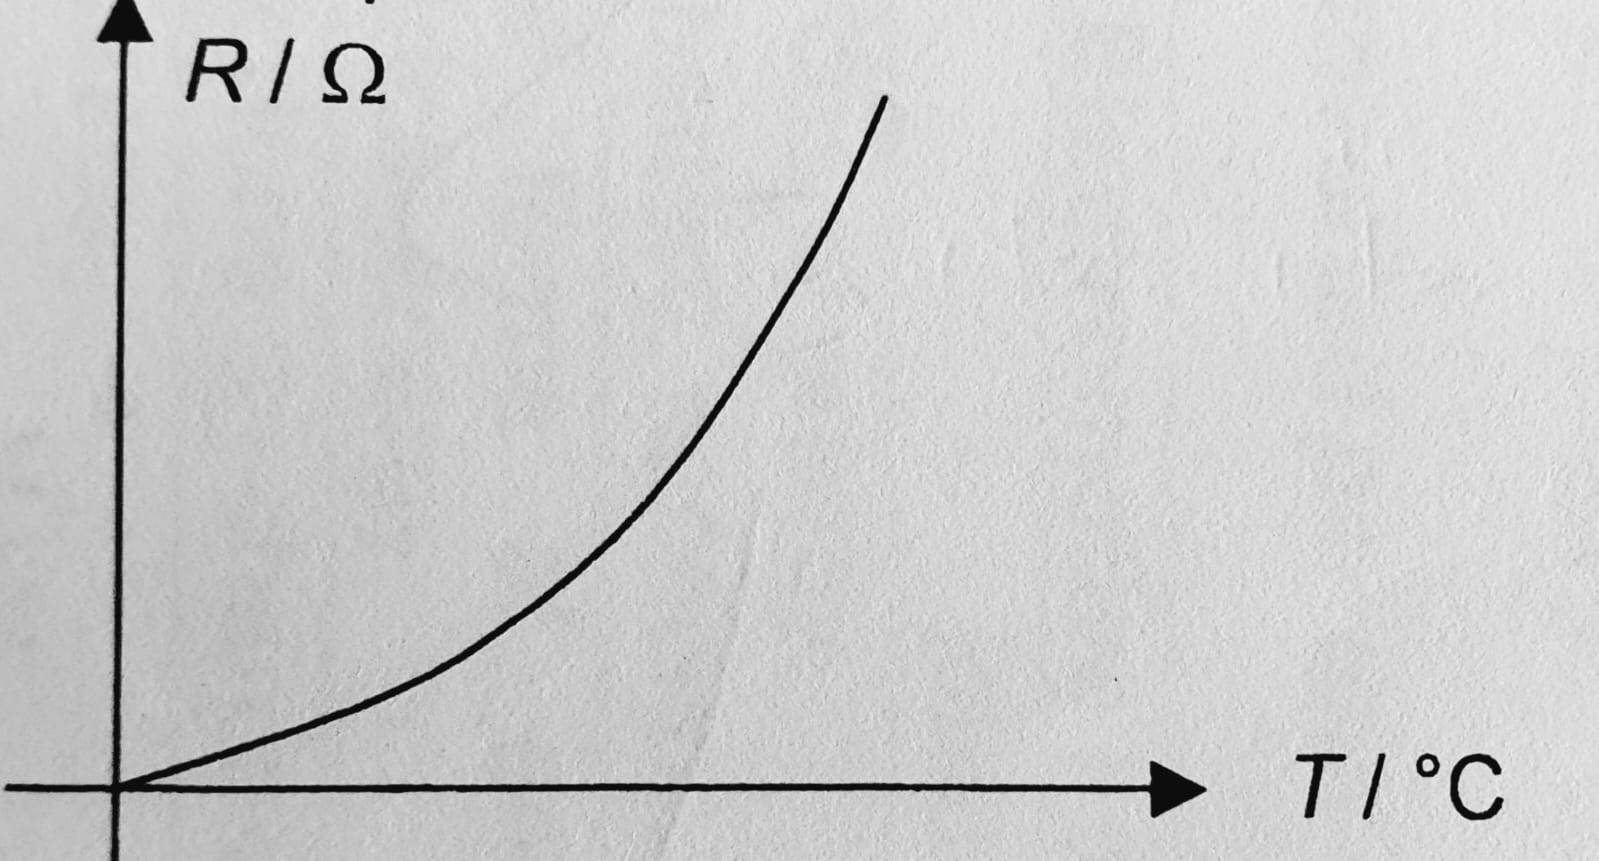
\includegraphics[width=\textwidth]{../images/Filament Lamp Resistance.jpg}
        \end{minipage} &
        \begin{minipage}{0.3\textwidth}
            \begin{itemize}
                \item As \emph{current increases, power dissipated increases} since \(P=I^2R\). Heat is generated so \emph{equilibrium temperature rises} --- as electrons drift through the metal, they collide with the metal lattice and transfers energy to it. 
                \item The \emph{lattice ions vibrate more vigorously}. This \emph{hinders the flow} of `charge carriers'. Therefore, \emph{resistance is increased}.
                \item Ohmic conductors hence do \emph{not} obey Ohm's Law at \emph{high} voltages/currents.
            \end{itemize}
        \end{minipage}\\
        \hline
        \begin{minipage}{0.25\textwidth}
            Negative Temperature Coefficient (NTC) Thermistor
        \end{minipage} &  
        \begin{minipage}{0.3\textwidth}
            \begin{itemize}
                \item When \emph{p.d. increases}, \emph{current} through the thermistor also \emph{increases}, with \emph{increasing \(I\)-\(V\) ratio}.
                \item The \emph{resistance} of a thermistor \emph{decreases} with an \emph{increase} in \emph{temperature} (This is the meaning of NTC).
            \end{itemize} 
            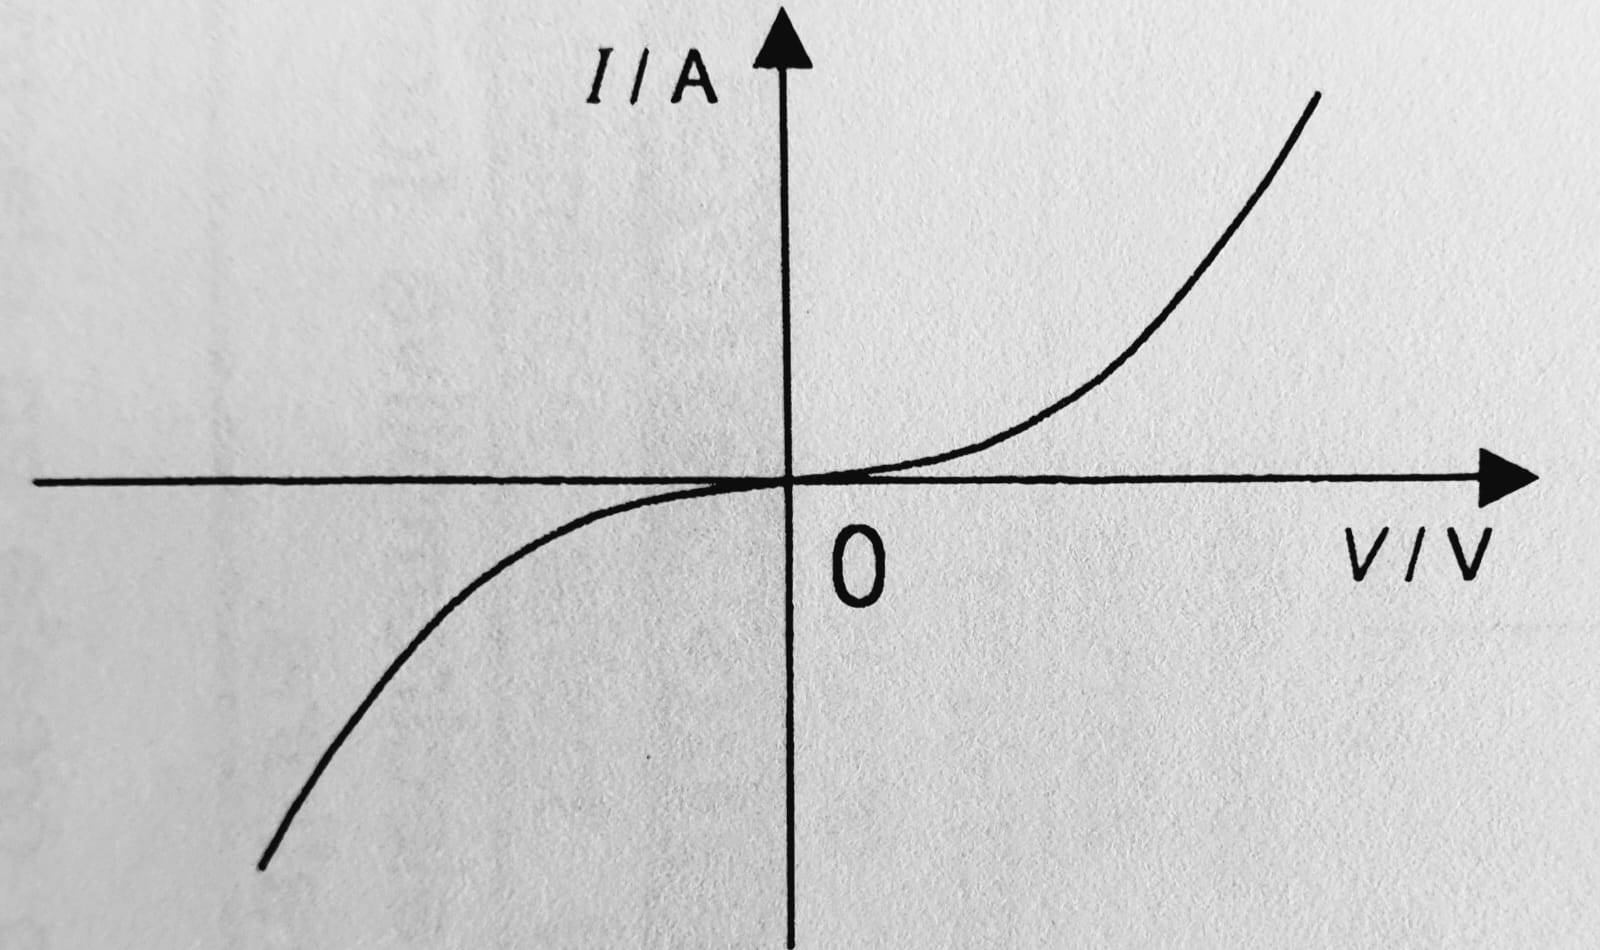
\includegraphics[width=\textwidth]{../images/NTC I-V.jpg}\\[-1mm]
            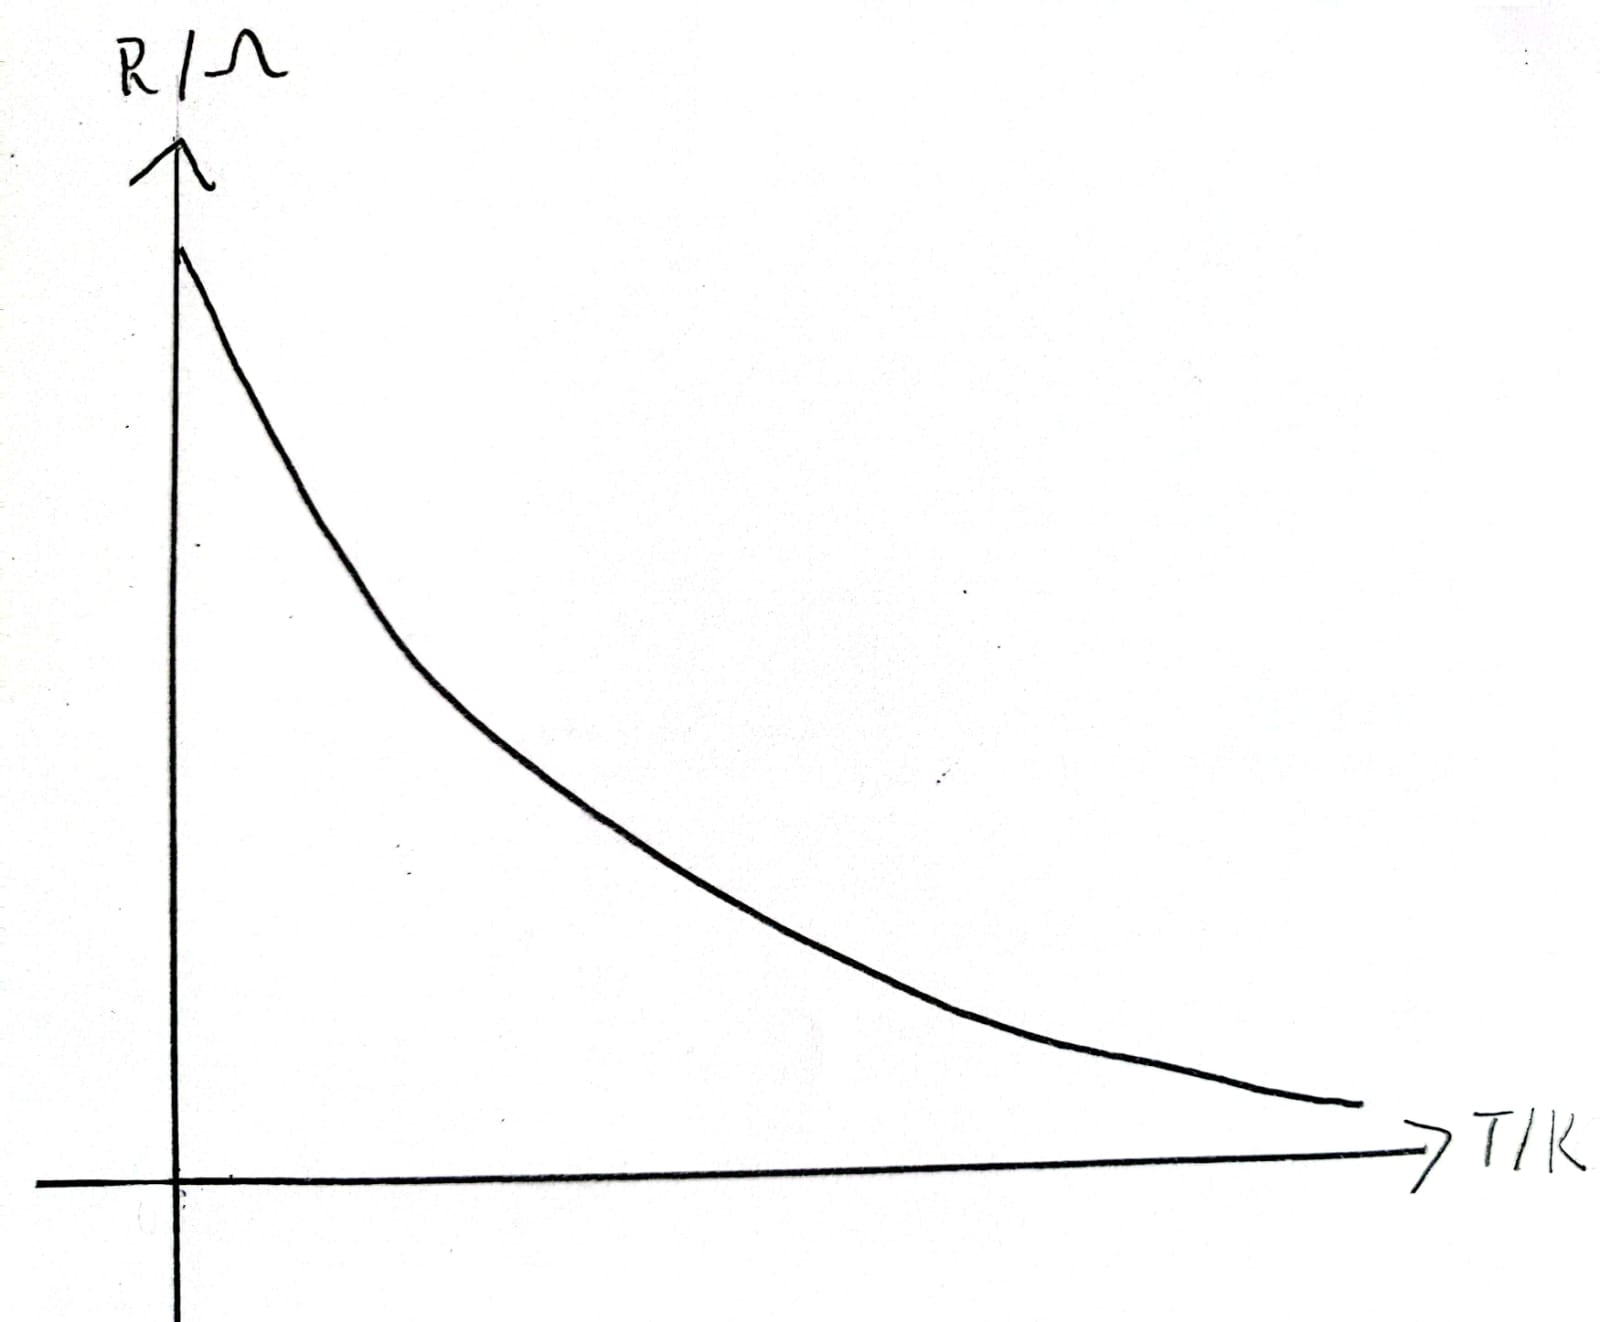
\includegraphics[width=\textwidth]{../images/NTC Resistance.jpg}
        \end{minipage} &
        \begin{minipage}{0.3\textwidth}
            \begin{itemize}
                \item  As \emph{current increases}, \emph{power dissipated increases}. \emph{More heat} is generated, leading to a \emph{rise} in \emph{equilibrium temperature}.
                \item Thus, the \emph{mean kinetic energy} of the electrons and lattice ions \emph{increases}. So,
            \end{itemize}
            \begin{enumerate}
                \item The \emph{bonded electrons break free} from bonds, increasing the \emph{number} of `mobile charge carriers'. Therefore, \emph{resistance decreases}.
                \item The \emph{lattice ions vibrate more vigorously}, \emph{hindering the flow} of `mobile charge carriers'. Thence, resistance increases.  
            \end{enumerate} 
            \begin{itemize}
                \item The first effect is much more significant than the second. So, there is a net \emph{decrease in resistance}.
            \end{itemize}
        \end{minipage}\\
        \hline
    \end{longtable}
    The images above come from \ref{RVHS}.
    \newpage
    \item The \emph{electromotive force} (e.m.f) of a \emph{source} is defined as the amount of \emph{energy converted} from \emph{non-electrical} forms of energy to \emph{electrical} energy \emph{per unit charge} as the \emph{charge passes through a complete circuit}.
    \item Internal resistance: the p.d. across a component is given by \(V=E-Ir\).
    \item Power dissipated \(P=IV\).
    \item Power delivered is \emph{maximum } when \(R=r\), such that 
    \[P_{\text{max}}=\frac{E^2}{4r}.\]
    \item Efficiency of the source
    \begin{itemize}
        \item \emph{Increases} when external load/\emph{resistance increases}.
        \item Is halved when \(R=r\).

        \emph{Note:} Maximum power \(\neq\) maximum efficiency.
    \end{itemize}
\end{itemize}

\chapter{Electric Fields}
\begin{itemize}
    \item \emph{Coulomb's Law} states that the \emph{magnitude} of the \emph{electric force} between two \emph{point charges} is directly proportional to the product of the charges, and inversely proportional to the square of their separation.
    \item The constant \(\varepsilon_0\) is the permittivity of \emph{free space} (\(\varepsilon_0\) is applicable only in air or a vacuum).
    \item Sign of \(F_E\):
    \begin{center}
        \begin{tabular}{|Sc|Sc|}
            \hline
            \(F_E\) & Direction\\
            \hline
            Positive & Repulsive\\
            \hline
            Negative & Attractive\\ 
            \hline
        \end{tabular}  
    \end{center}
    
  \item The sign of the electric force does \emph{not} represent the \emph{direction} of the electric force. It only informs us whether the force is attractive or repulsive. So, when calculating the \emph{resultant} electric force, we need to account for the direction ourselves. 
    \item Comparison between E-fields and G-fields: 
    \begin{center}
        \resizebox{0.942\textwidth}{!}{\begin{tabular}{|Sc|Sc|Sc|}
            \hline
            Sim/Diff & E-field & G-field\\
            \hline
            S & 
            \multicolumn{2}{Sc|}{\begin{minipage}{0.8\textwidth}
            For both Column's Law and Newton's Law of Gravitation, \(r\) is the \emph{center to center separation} of the objects.
            \end{minipage}}\\
            \hline
            S & 
            \multicolumn{2}{Sc|}{\begin{minipage}{0.8\textwidth}
            By Newton's Third Law, the \emph{forces} that masses and charges exert on each other is \emph{equal in magnitude} and \emph{opposite in direction}.
            \end{minipage}}\\
            \hline
            D & 
            \begin{minipage}{0.4\textwidth}
                Electric Forces can be \emph{attractive or repulsive}.
            \end{minipage} &
            \begin{minipage}{0.4\textwidth}
                Gravitational forces are \emph{always attractive}.
            \end{minipage}\\
            \hline 
    \end{tabular}}
    \end{center}
    \item An \emph{electric field} is a \emph{region in space} where a \emph{charge experiences an electric force}.
    \item How to draw electric field lines: 
    \begin{itemize}
        \item \emph{Lines cannot intersect} one another.
        \item Lines must \emph{begin from positive charges} and \emph{end on negative charges}.
        \item Arrows show the \emph{direction of force} exerted on a positive test charge.
        \item The \emph{greater} the electric field strength, the \emph{closer} together field lines are drawn.
        \item Lines leave/end on \emph{conducting surfaces} at \emph{right angles}
    \end{itemize}
    % POINT CHARGE +1
    \resizebox{0.942\textwidth}{!}{\begin{tikzpicture}
    \foreach \i [evaluate={\angle=(\i-1)*360/\NE;}] in {1,...,\NE}{
      \draw[EFieldLineArrow={0.6}] (0,0) -- (\angle:\R);
    }
    \draw[charge+] (0,0) circle (7pt) node[black,scale=0.8] {$+q$};
  \end{tikzpicture}
  % POINT CHARGE -1
  \begin{tikzpicture}
    \foreach \i [evaluate={\angle=(\i-1)*360/\NE;}] in {1,...,\NE}{
      \draw[EFieldLineArrow={0.5}] (\angle:\R) -- (0:0);
    }
    \draw[charge-] (0,0) circle (7pt) node[black,scale=0.8] {$-q$};
  \end{tikzpicture}
  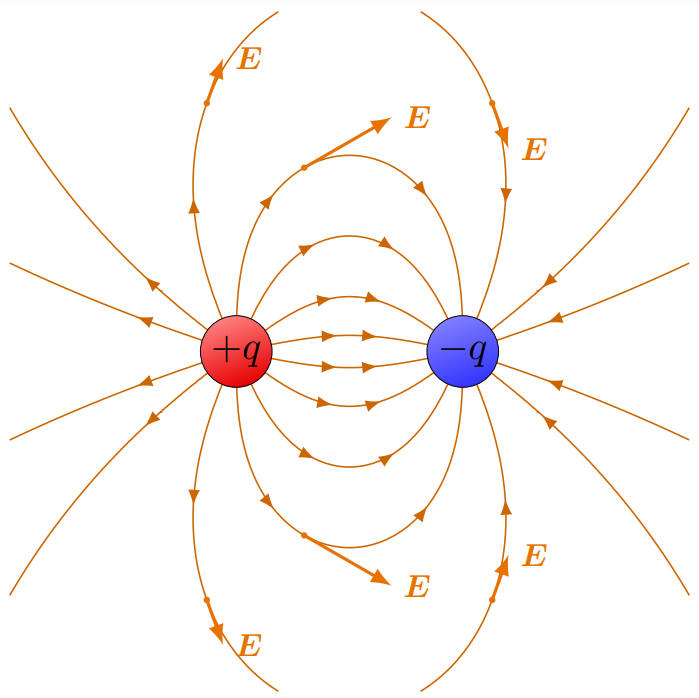
\includegraphics[width=0.25\textwidth]{../images/2 charges.png}
  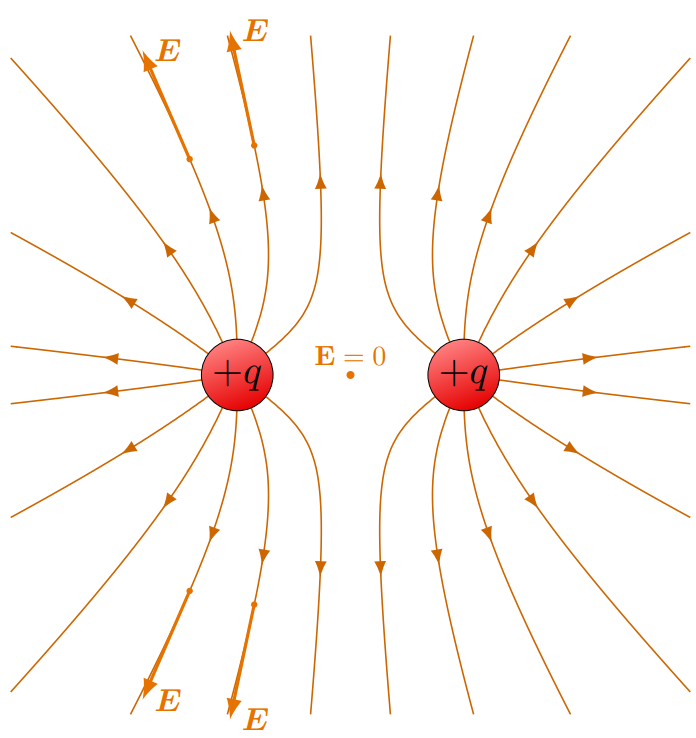
\includegraphics[width=0.25\textwidth]{../images/2repellingcharges.png}}
  \captionsetup{type=figure}
  \caption[figure]{\ref{Electric field lines of a point charge}, \ref{Electric field lines of two charges} Electric field lines of point charges and two interacting charges.}
  \begin{center}
    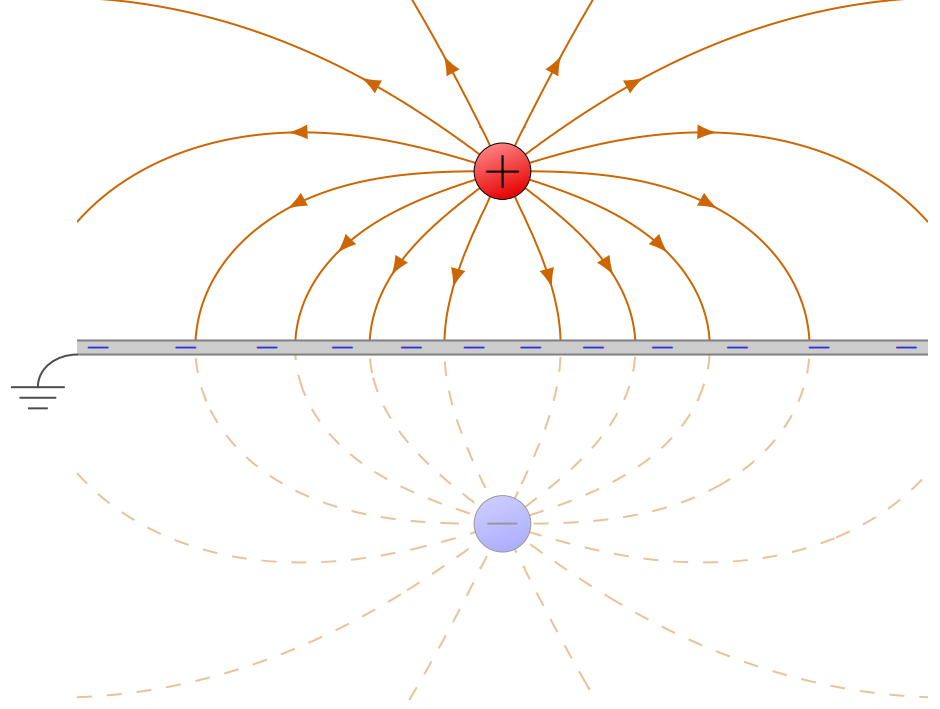
\includegraphics[width=0.5\textwidth]{../images/E-fieldPlate.png}
    \captionsetup{type=figure}
    \caption[figure]{\ref{Interaction of a point charge with a charged plate} Interaction of a point charge with a charged plate.}
  \end{center}
  \item The \emph{electric field strength} at a point is defined as the \emph{electric force} per \emph{unit positive charge} acting on a small stationary test charge placed at that point.
  \begin{center}
    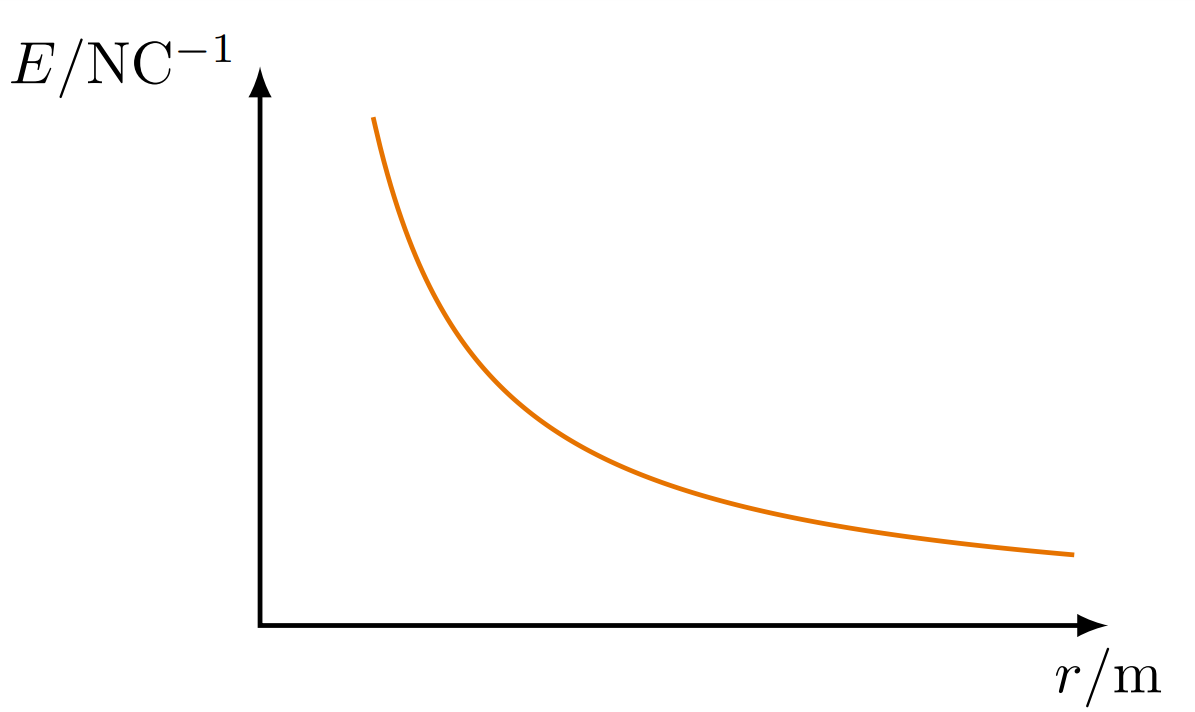
\includegraphics[width=0.5\textwidth]{../images/ElectricFieldStrengthPlot.png}
    \captionsetup{type=figure}
    \caption[figure]{\ref{Electric field plots} Electric field strength of a positive point charge}
  \end{center}
  \item Charge distribution on a conducting sphere: 
  \begin{itemize}
    \item Excess charges are forced to the surface of the conductor until the electric field inside the conductor is zero. 
    \item \emph{Outside} the conductor, the electric field is the \emph{same} as that of an isolated point charge equal to the excess charge. 
  \end{itemize}
  \item Properties of conductors in \emph{electrostatic equilibrium}:
  \begin{itemize}
    \item The \emph{electric field is zero inside} a conductor (regardless of shape).
    \item So, the \emph{entire conductor} is at the \emph{same potential}.
    \item Just outside the conductor, the e-field lines are \emph{perpendicular to its surface}, starting and ending on charges on the surface.
    \item \emph{Excess charges} resides exclusively on \emph{the surfaces} of a conductor.
  \end{itemize}
  \item Electric field strength between two charged parallel plates is uniform everywhere between the plates, except at both ends of the plates. 
  \item Also, \emph{charges} between the plates experience \emph{uniform acceleration}.
  \begin{center}
    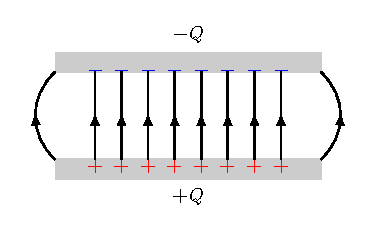
\includegraphics[scale=1]{../images/ParallelPlates/testing.pdf}
    \captionsetup{type=figure}
    \caption[figure]{\ref{Electric field lines between parallel plates} Electric field lines between parallel plates.}
  \end{center}
  \item Magnitude of electric field strength between the plates:
  \[E=\frac{dV}{dr}=\frac{\Delta V}{d}.\]
  \item The \emph{electric potential energy} of a point charge in an electric field is defined as the \emph{work done by an external agent} in bringing the point charge from infinity to that point (without any net change in kinetic energy). 
  \item The \emph{electric potential} at a point in an electric field is defined as the \emph{work done} per unit \emph{positive} charge, by an external agent, in bringing a \emph{small} test charge from infinity to that point (without any net change in kinetic energy). 
  \item Let \(U\) be the electric potential energy, and \(V\) the electric potential. Then,
  \[U=qV \qquad\text{and}\qquad \Delta U=q\Delta V.\]
  \item ~
  \begin{center}
    \begin{tikzcd}[row sep=large, column sep=large]
        U=\frac{Qq}{4\pi\varepsilon_0r} \arrow{r}{-\frac{\text{d}}{\text{d}r}} \arrow[swap]{d}{\frac{1}{q}} & F_E=\frac{Q_1Q_2}{4\pi\varepsilon_0r^2} \arrow[swap]{d}{\frac{1}{q}} \\
        V=\frac{Q}{4\pi\varepsilon_0r} \arrow{r}{-\frac{\text{d}}{\text{d}r}} & E=\frac{Q}{4\pi\varepsilon_0r^2}\\
    \end{tikzcd}
  \end{center}
  \item The \emph{electric potential} at a point \(X\) due to a \emph{system} of point charges \(q_i\) is the algebraic sum of the electric potential \(V_i\) due to each individual charge \(q_i\) which is distance \(r_i\) away from \(X\). That is, 
  \[V=\sum_{i}{V_i}=\sum_{i}^{}{\frac{q_i}{4\pi\varepsilon_0r_i}}.\]
  \item The \emph{potential energy} of a \emph{system} of charges \(q_i\) is the work done to assemble it. This is the sum of energies \(U_{ij}\) needed to bring each charge \(q_i\) to the charges \(q_j\) (for \(i>j\)) already present. In other words letting \(r_{ij}\) be the distance of \(q_i\) from \(q_j\), we have 
  \[U=\sum_{i>j}{U_{ij}}=\sum_{i>j}^{}{\frac{q_iq_j}{4\pi\varepsilon_0r_{ij}}}.\] 
\end{itemize}
\begin{center}
    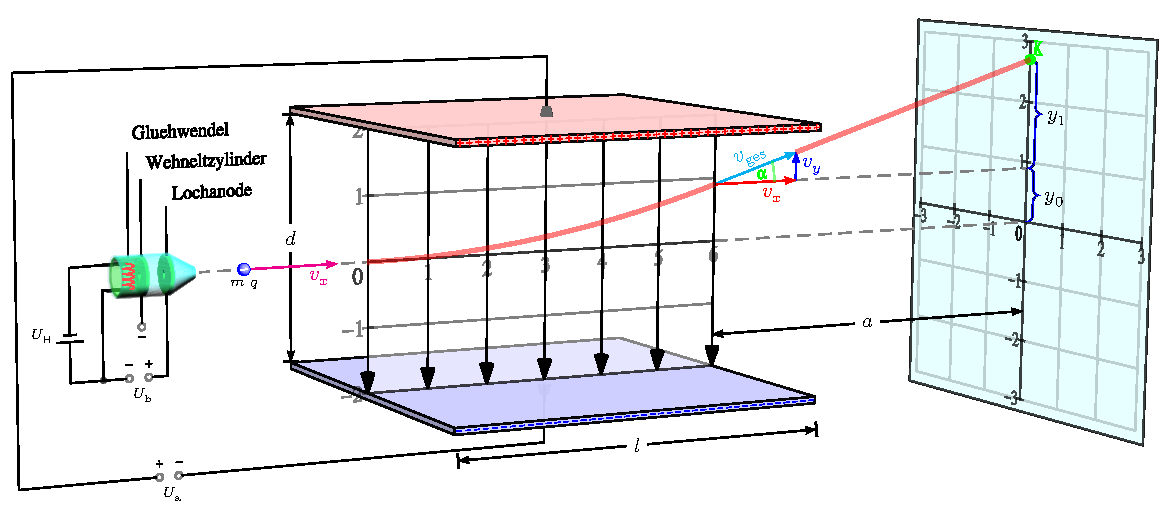
\includegraphics[width=\textwidth]{../images/Electron-Deflection/Bahn-Kondensator (1).pdf}
    \captionsetup{type=figure}
    \caption[figure]{\ref{Electron deflection} Deflection of an electron.}
\end{center}

\chapter{D.C. Circuits}
\begin{center}
    \begin{tabular}{|Sc|Sc|Sc|}
        \hline
        Property & Series & Parallel\\
        \hline
        Current & \(I_1=I_2=\cdots=I_n\) & \(I_i=\dfrac{E}{R_i}\)\\
        \hline
        Resistance & \(R_{\text{effective}}=R_1+R_2+\cdots+R_n\) & \(\dfrac{1}{R_{\text{effective}}}=\dfrac{1}{R_1}+\dfrac{1}{R_2}+\cdots+\dfrac{1}{R_n}\)\\
        \hline
        Voltage & \(V_i=\dfrac{R_i}{R_T}\cdot E\) & \(E=V_1=V_2=\cdots=V_n\).\\
        \hline
    \end{tabular}
\end{center}
\begin{itemize}
    \item For \(n\) identical resistors in parallel, which are each of resistance \(R\), we have \(R_{\text{effective}}=R/n\). Furthermore, the effective resistance is at most the resistance of the smallest resistor, i.e. \(R_{\text{effective}}\leq R_i\) for each \(i\). In fact, the inequality is strict when the number of resistors in parallel \(n\geq 2\).
    \item To resolve tricky systems of resistors, use the fact that electric potential is constant along a wire.
    \begin{center}
        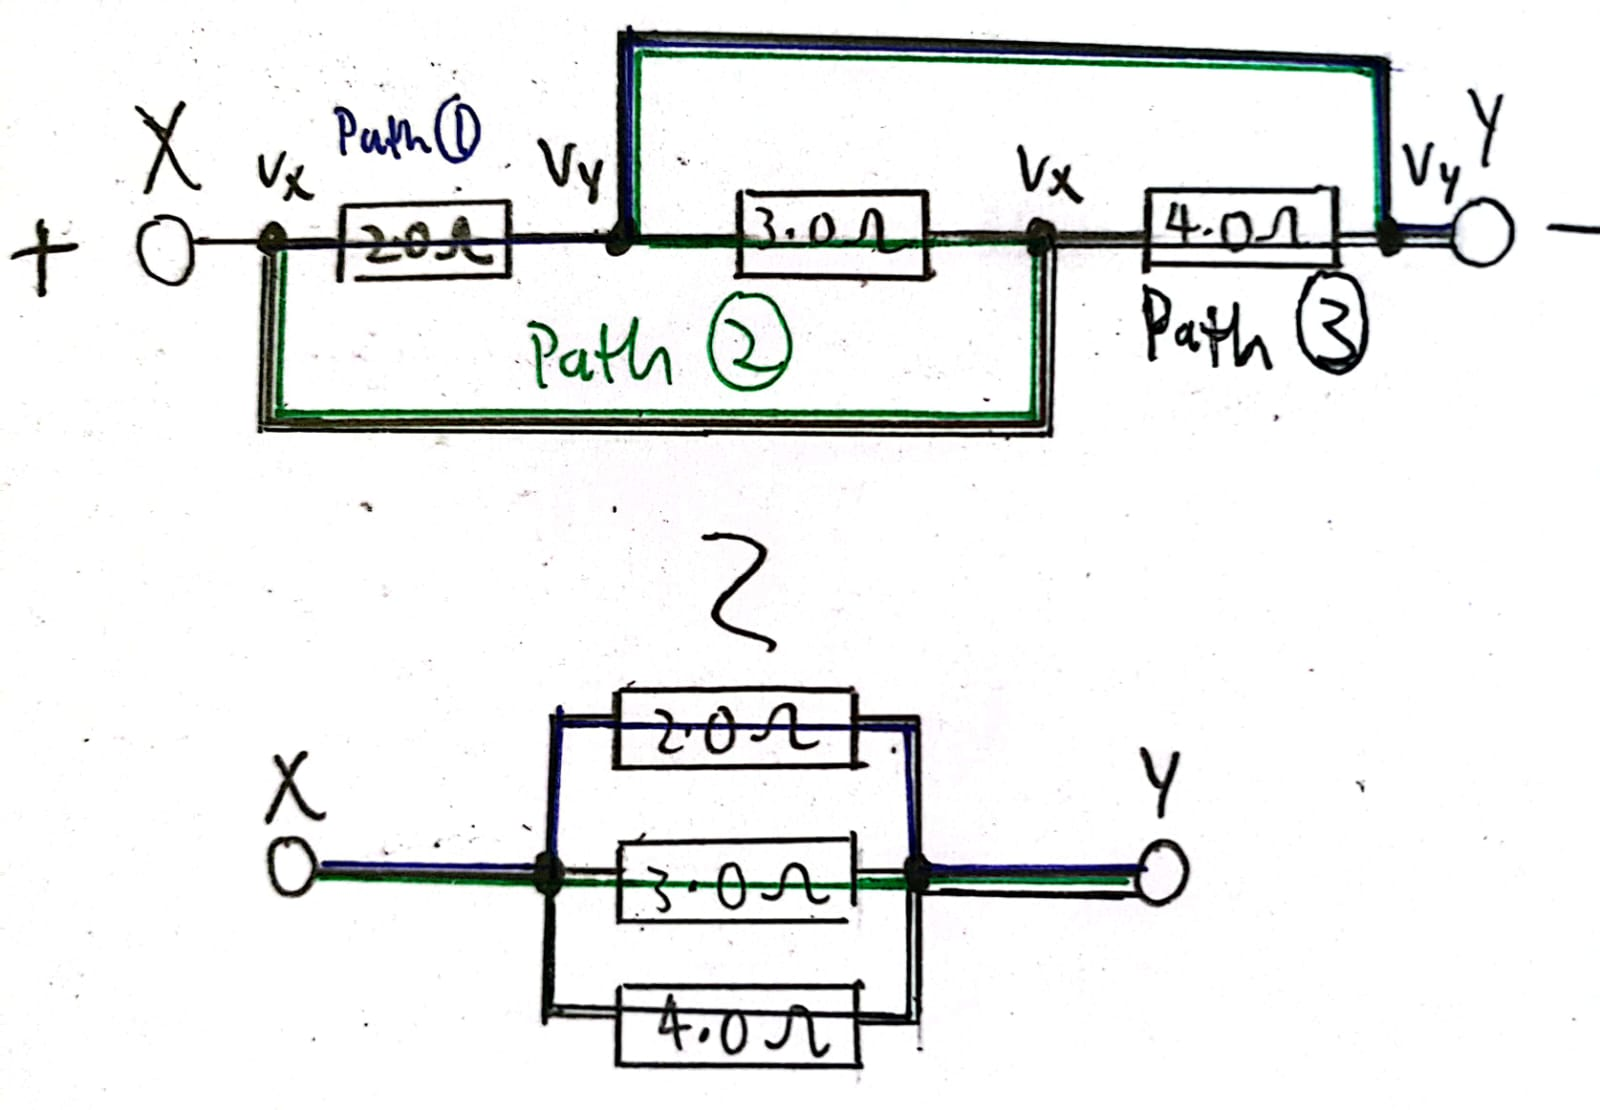
\includegraphics[width=0.93\columnwidth]{../images/DC-Circuits-Resistors.jpg}
        \captionsetup{type=figure}
        \caption[figure]{\ref{RVHS} Some tricky ciruits.}
    \end{center}
    \item Potentiometer:
    \begin{itemize}
        \item E.m.f. of driver cell is more than that of the unknown cell, \(E\).
        \item The direction of charge flow for the primary and secondary circuits are opposite. i.e. the positive/negative terminals should `point' towards each other.
        \item The potential difference \(V\) across length \(L\) of a resistance wire is directly proportional to \(L\).
        \item Consider the following circuit. When the galvanometer reads zero, the e.m.f. of the unknown cell is \(E_{AJ}\), where 
        \[\frac{E_{\text{AJ}}}{E}=\frac{L_{\text{AJ}}}{L_{\text{AB}}}=\frac{R_{\text{AJ}}}{R_{\text{AB}}}.\]
        \begin{center}
            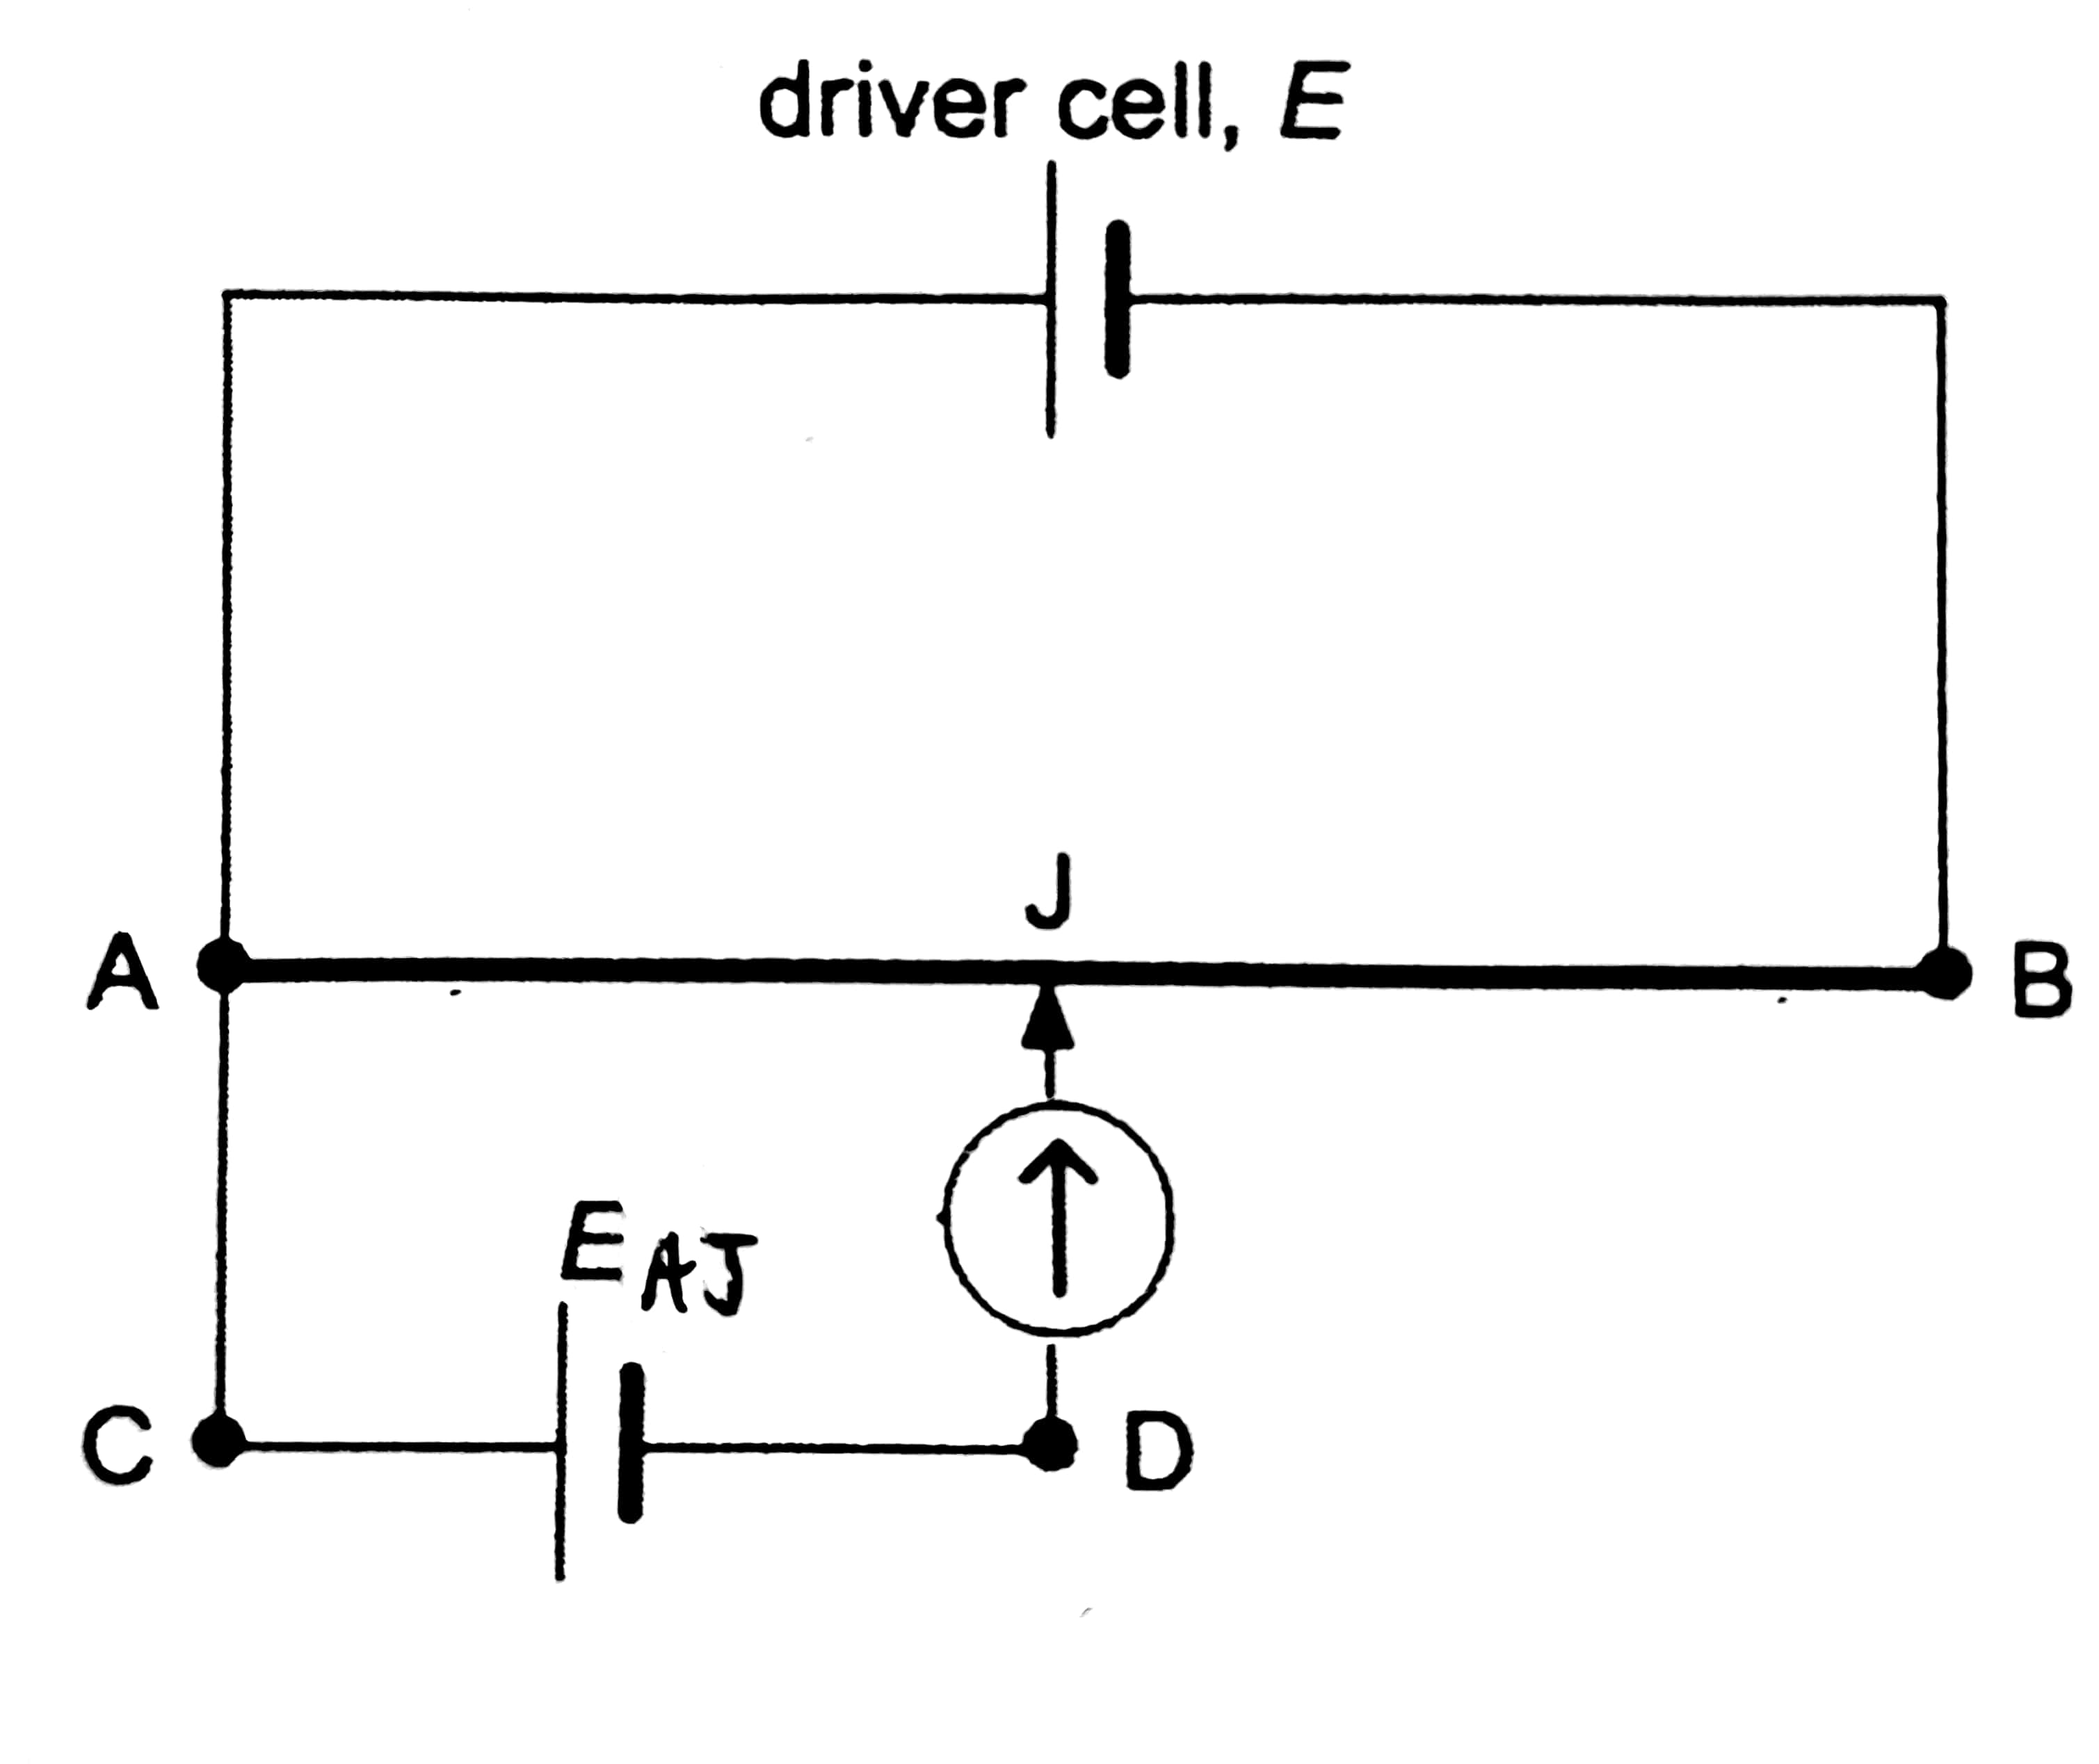
\includegraphics[width=0.4\columnwidth]{../images/DC-Circuits-Potentiometer-1.jpg}
            \captionsetup{type=figure}
            \caption[figure]{\ref{RVHS} An illustration of a potentiometer.}
        \end{center}
        \item In the circuit below, the internal resistance \(r\) satisfies
        \[\frac{L_{AJ_2}}{L_{AJ_1}}=\frac{R}{R+r}.\]
        \begin{center}
            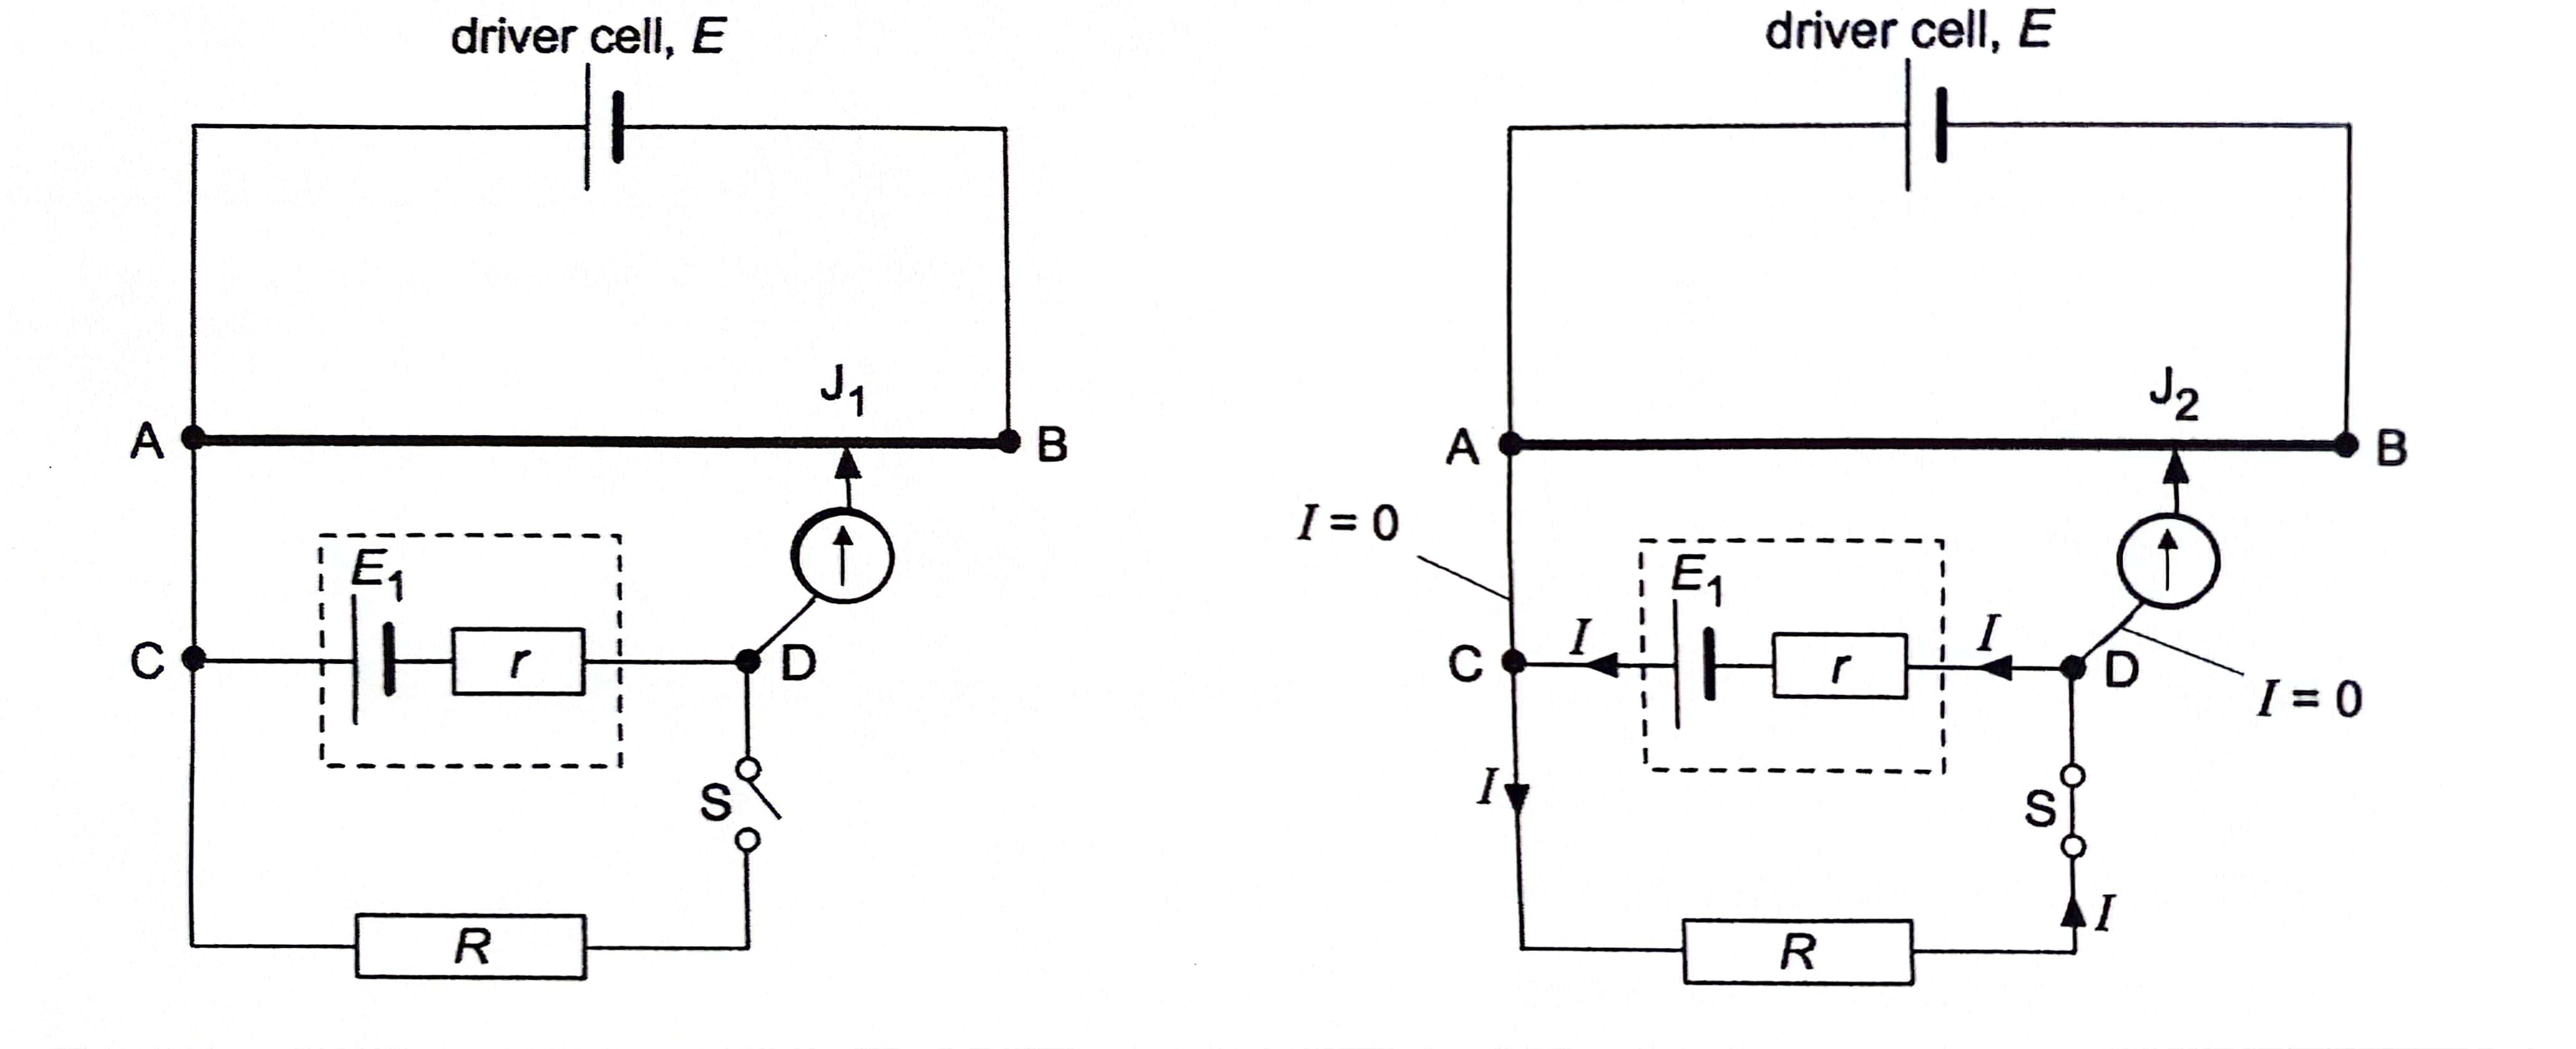
\includegraphics[width=0.88\columnwidth]{../images/DC-Circuits-Potentiometer-2.jpg}
            \captionsetup{type=figure}
            \caption[figure]{\ref{RVHS} Some more illustrations of potentiometers.}
        \end{center}
        For the diagram to the left, why \(V_{CD}=V_{AJ_1}\) is easily seen from the diagram below.
        \begin{center}
            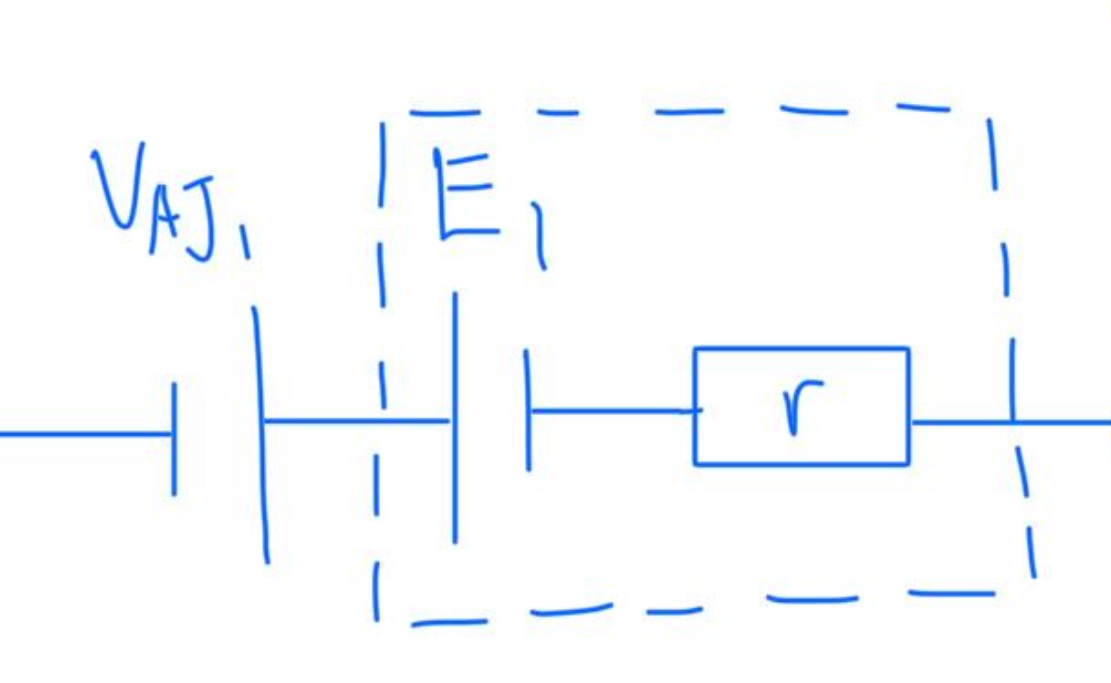
\includegraphics[width=0.3\columnwidth]{../images/D.C.-Voltage-Cancelling-Each-Other.png}
            \captionsetup{type=figure}
            \caption[figure]{\ref{Me} Part CD of the circuit.}
        \end{center}
    \end{itemize}
\end{itemize}

\chapter{Electromagnetism}
\begin{center}
    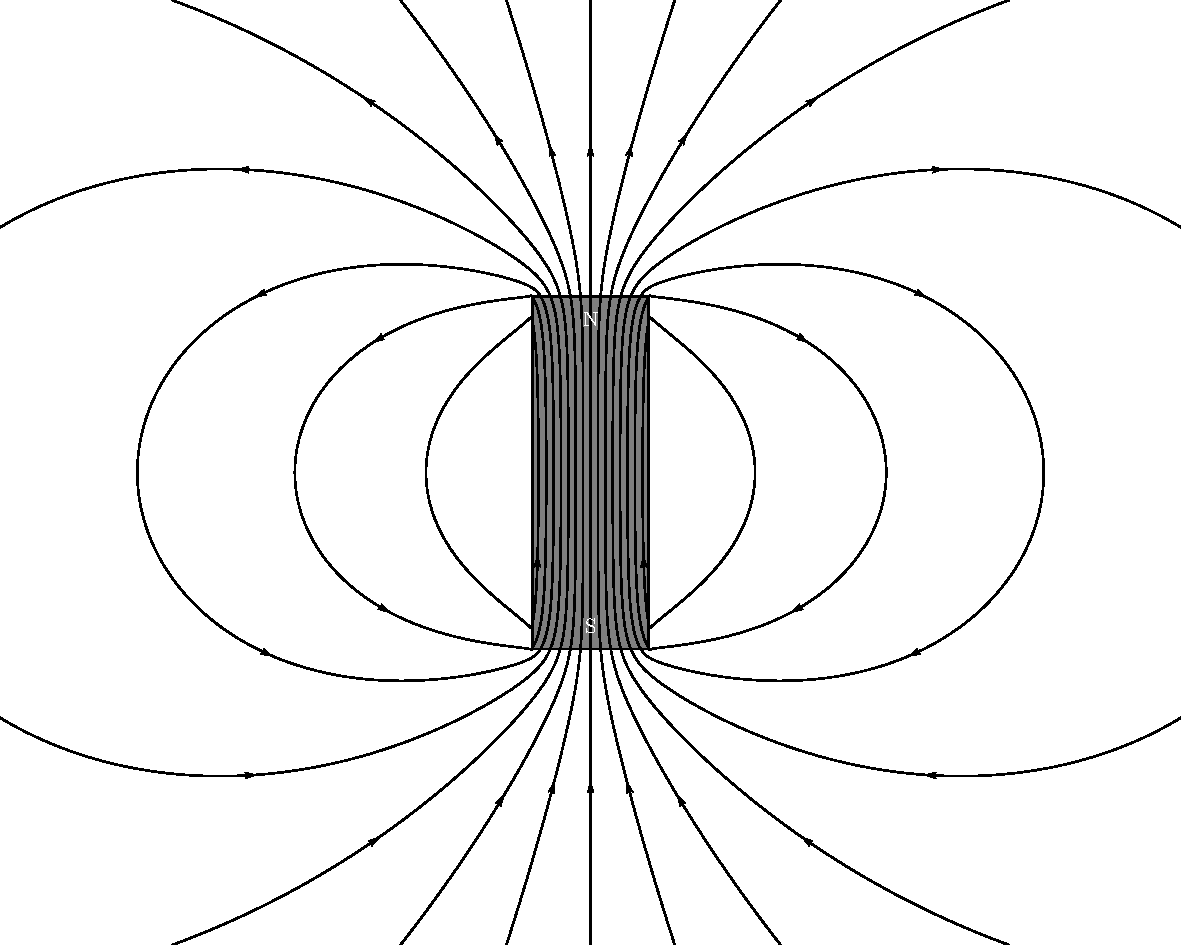
\includegraphics[width=0.8\textwidth]{../images/Bar-Magnet/Bar-Magnet.pdf}
    \captionsetup{type=figure}
    \caption[figure]{\ref{Magnetic field produced by a bar magnet} Magnetic field produced by a bar magnet.}
\end{center}
\begin{itemize}
    \item A \emph{magnetic field} is a \emph{region of space} where a magnetic pole, moving charged particle or current-carrying conductor will \emph{experience a magnetic force}.
    \item Normally, a magnetic field points from north-to-south. However, \emph{inside} a magnet, the magnetic field points south-to-north. 
    \item \emph{Magnetic flux density} is defined as the \emph{force per unit current per unit length} acting on an \emph{infinitely long current-carrying conductor} placed \emph{perpendicularly} to the magnetic field.
    \item Dots and crosses as indicators of direction:
    \begin{center}
        \begin{tabular}{|Sc|Sc|}
            \hline
            \Large \(\bigotimes\) & Into the page\\
            \hline
            \Large \(\bigodot\) & Out of the page\\
            \hline
        \end{tabular}
    \end{center}
    \newpage
    \item Left and right hand rules:
    \begin{center}
        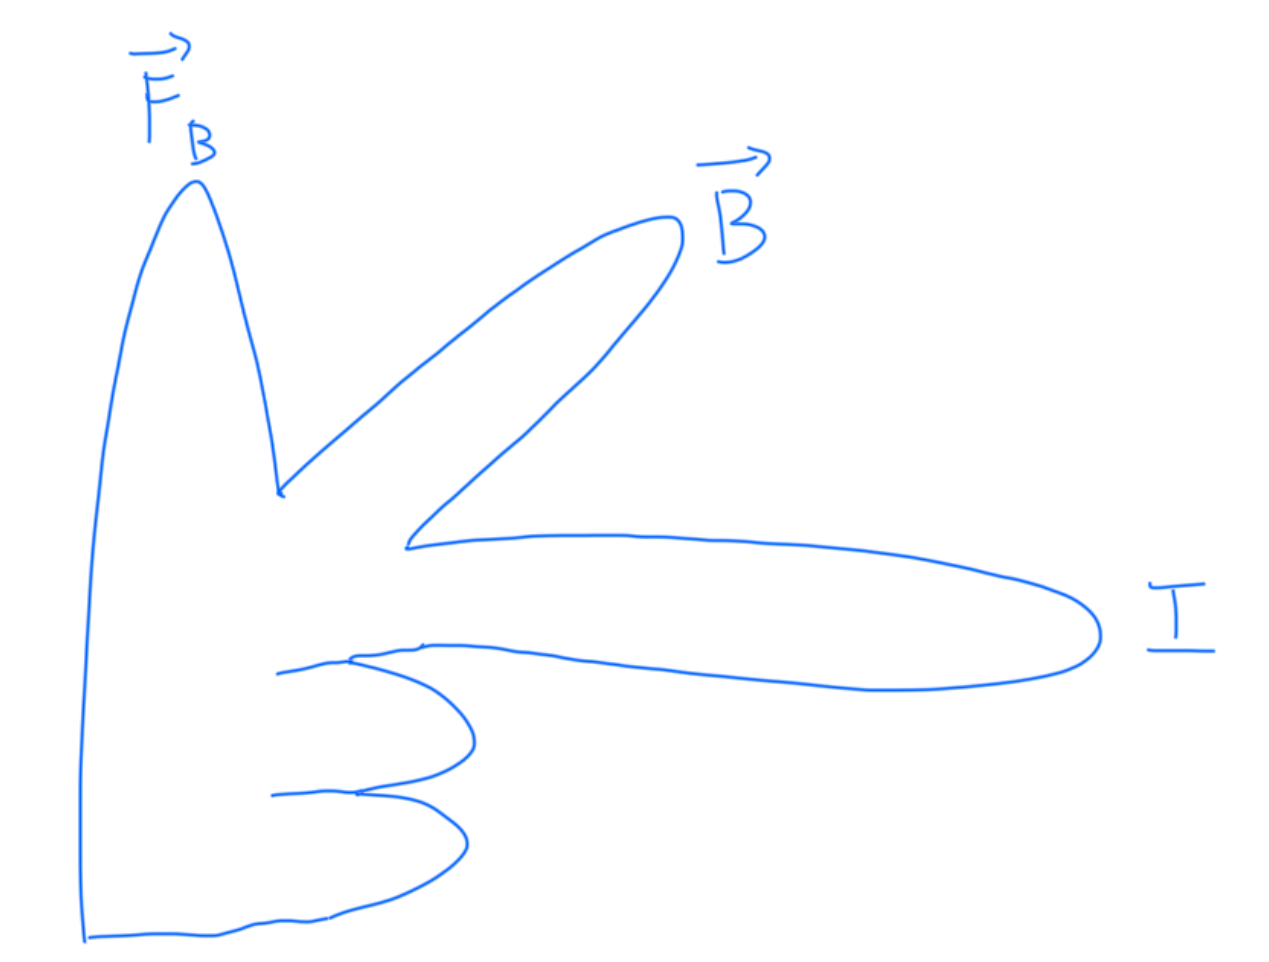
\includegraphics[width=0.5\textwidth]{../images/Left-Right-Hand-Rules/Left-hand-rule.png}
        \hspace{2cm}
        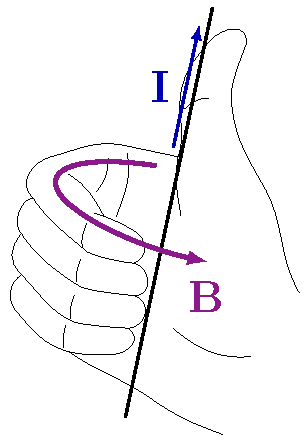
\includegraphics[width=0.28\textwidth]{../images/Left-Right-Hand-Rules/Right-hand-rule.pdf}
        \captionsetup{type=figure}
        \caption[figure]{\ref{Left and right hand rules} Left and right hand rules.}
    \end{center}
    \item At any point some perpendicular distance \(d\) from the center of an \emph{infinitely long straight} current-carrying conductor, the magnitude of the magnetic flux is given by
    \[B=\frac{\mu_0I}{2\pi d}.\]
    Here, \(\mu_0=4\pi\cdot 10^{-7}\) is the permeability of free space.
    \begin{center}
        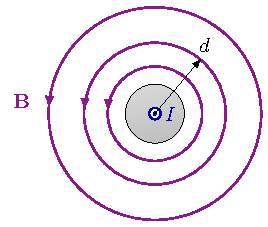
\includegraphics[width=0.5\textwidth]{../images/Current-Carrying-Wire/Current-Carrying-Wire.pdf}
        \captionsetup{type=figure}
        \caption[figure]{\ref{Current in a wire} Current in a wire.}
    \end{center}
    \item At the center of a flat circular coil with \(N\) turns, radius \(r\), and current \(I\) flowing through it, the magnitude of the magnetic flux density is given by 
    \[B=\frac{\mu_0NI}{2r}.\]
    \begin{center}
        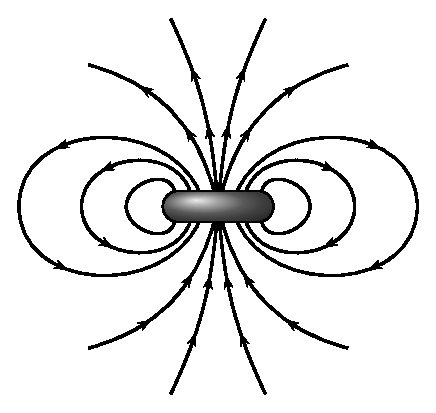
\includegraphics[width=0.5\textwidth]{../images/Flat-Circular-Coil/Flat-Circular-Coil.pdf}        \captionsetup{type=figure}
        \caption[figure]{\ref{Flat circular coil} Current in a flat circular coil.}
    \end{center}
    \item Suppose we have an ideal (having infinite length) solenoid of \(n=N/L\) number of turns per unit length, which has a current \(I\) flowing through it. Then, the magnitude of the uniform magnetic flux density at its center is given by 
    \[B=\mu_0nI.\]
    \begin{center}
        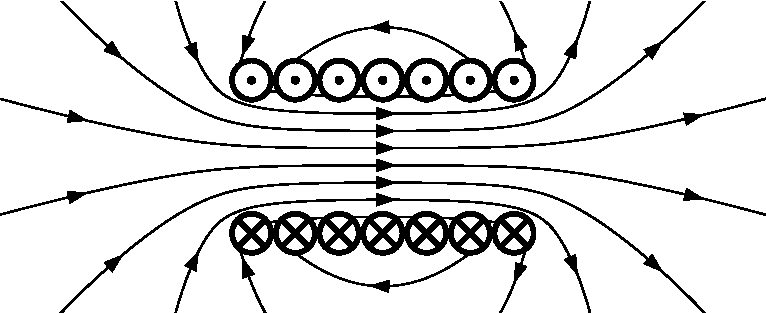
\includegraphics[width=0.9\textwidth]{../images/Solenoid.pdf}
        \captionsetup{type=figure}
        \caption[figure]{\ref{Solenoid} Current in a solenoid and the magnetic field produced.}
    \end{center}
    \item A set of coils can be considered to be a solenoid when the radius of said coils is negligible compared to their length. 
    \item The addition of a ferrous core, of permeability \(\mu\), into a solenoid increases the magnetic flux density there, which is given by 
    \[B=\mu nI.\]
    \item Say we have a straight current-carrying conductor of length \(l\) with current \(I_\perp\) flowing perpendicular to the magnetic field. Then for any point on that conductor that experiences a magnetic flux of density \(B\), 
    \[F_B=BI_\perp l.\]
    \newpage
    \item ~
    \begin{center}
        \begin{tabular}{|Sc|Sc|}
            \hline
            Direction of Current in Two Wires & Direction of Net Magnetic Force\\
            \hline
            Same & Attractive\\
            \hline
            Opposite & Repulsive\\
            \hline
        \end{tabular} 
        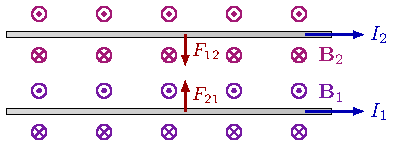
\includegraphics[scale=1.5,page=1]{../images/Two-Current-Carrying-Wires/Two-Current-Carrying-Wires.pdf}

        \includegraphics[scale=1.5,page=2]{../images/Two-Current-Carrying-Wires/Two-Current-Carrying-Wires.pdf}
        \captionsetup{type=figure}
        \caption[figure]{\ref{Two current carrying conductors} Current carrying conductors in parallel.}
    \end{center}
    \item A charge \(q\) moving at speed \(v_\perp\) perpendicular to the magnetic field, of flux density \(B\), experiences a magnetic force of magnitude
    \[F_B=qv_\perp B.\]
    \item Notice that the charged particle above travels in circular motion, with radius and period
    \[r=\frac{mv}{Bq}\qquad\text{and}\qquad T=\frac{2\pi m}{qB}.\]
    \item Velocity selector. Suppose we have a velocity selector with a uniform magnetic field, of flux density \(B\) out of (or into) the paper. Further assume there is an electric field of strength \(E\) rightwards (or leftwards) in the selector. This is illustrated in \hyperlink{Fig-15.7}{Fig 15.7}. Then, for a charged particle perpendicular to both fields to pass (undeflected) through the slits, \(F_E=F_B\). This simplifies to 
    \[v=\frac{E}{B}.\]
    \begin{center}
        \hypertarget{Fig-15.7}{}
        \begin{minipage}{0.9\textwidth}
            \centering
            \raisebox{-0.5\height}{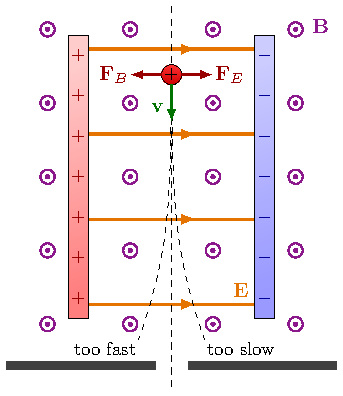
\includegraphics[width=0.45\textwidth,page=1]{../images/Velocity-Selector/Velocity-Selector.pdf}}
            \hspace*{.2in}
            \raisebox{-0.5\height}{\includegraphics[width=0.5\textwidth,page=2]{../images/Velocity-Selector/Velocity-Selector.pdf}}
            \captionsetup{type=figure}
            \caption[figure]{\ref{Velocity selector} An illustration of a velocity selector.}
          \end{minipage}
    \end{center}
\end{itemize}
\newpage
Some nice images:
\begin{center}
    \includegraphics[angle=90,width=\textwidth]{../images/Bar-Magnet/Cropped/1.pdf}
    \includegraphics[angle=90,width=\textwidth]{../images/Bar-Magnet/Cropped/2.pdf}
    \includegraphics[width=0.49\textwidth]{../images/Bar-Magnet/Cropped/3.pdf}
    \includegraphics[width=0.49\textwidth]{../images/Bar-Magnet/Cropped/4.pdf}
    \captionsetup{type=figure}
    \caption[figure]{\ref{Magnetic field produced by a bar magnet} Magnetic fields produced by two bar magnets.}
\end{center}
\chapter{Electromagnetic Induction}
\begin{itemize}
    \item \emph{Magnetic flux} is the \emph{product} of \emph{an area} and the component of \emph{magnetic flux density perpendicular} to that area.
    \item In other words, let \(A\) be an area in a uniform magnetic field, of flux density \(B_\perp\) perpendicular to \(A\). Then, the magnetic flux \(\Phi\) through \(A\) is
    \[\Phi=B_\perp A.\]
    \item The area \(A\) here is a \emph{vector}! When we flip it through \(\pi\) radians, the magnetic flux through it is now \(-\Phi=-B_\perp A\). 
    \item \emph{One weber} is the \emph{magnitude of magnetic flux} through an \emph{area of} \(1\text{m}^2\) when a \emph{magnetic field of} \(1\text{T}\) acts \emph{perpendicularly into} the area.
    \item \emph{Magnetic flux linkage} through a coil is defined as the \emph{product} of the \emph{number of turns} of the coil and the magnetic flux through each turn of the coil.
    \item The magnetic flux through a coil of \(N\) turns is hence
    \[N\Phi=NB_\perp A.\]
    \item \emph{Faraday's Law of Electromagnetic Induction} states that the \emph{e.m.f. induced} in a \emph{conductor} is \emph{directly proportional} to the \emph{rate of change of magnetic flux linkage}.
    \item \emph{Lenz's Law} states that the \emph{direction of the induced e.m.f.} is such that it may produce \emph{an effect} that \emph{opposes the change} causing it.
    \item Lenz's Law is a consequence of conservation of energy. Mechanical work done to enable the change in magnetic flux linkage is converted into electrical energy.
    \item Faraday's and Lenz's Laws imply that the e.m.f generated is
    \[E=-(N\Phi)'=-(NB_\perp A)'.\]
    (The negative sign indicates that the induced e.m.f. opposes the change in magnetic flux linkage.)
    \begin{center}
        \includegraphics[width=0.4\textwidth,page=4]{../images/Lenz's-Law/Lenz's-Law.pdf}
        \includegraphics[width=0.45\textwidth,page=5]{../images/Lenz's-Law/Lenz's-Law.pdf}
        \includegraphics[width=0.4\textwidth,page=3]{../images/Lenz's-Law/Lenz's-Law.pdf}
        \captionsetup{type=figure}
        \caption[figure]{\ref{Lenz's Law} Examples of Lenz's Law in action.}
    \end{center}
    \item Motional e.m.f.: Suppose we have a circuit as shown in the bottom left of the following figure. Then, by Faraday's Law,
    \[\lvert E \rvert=\Phi'=B(\Delta A)=Blv.\]
    \begin{center}
        \begin{minipage}{0.9\textwidth}
            \centering
            \raisebox{-0.5\height}{\includegraphics[width=0.58\textwidth,page=1]{../images/Lenz's-Law/Lenz's-Law.pdf}}
            \hspace*{.2in}
            \raisebox{-0.5\height}{\includegraphics[width=0.37\textwidth,page=2]{../images/Lenz's-Law/Lenz's-Law.pdf}}
            \captionsetup{type=figure}
            \caption[figure]{\ref{Lenz's Law} Example of motional emf.}
          \end{minipage}
    \end{center}
    \item Conventions for polarity and when to use them.
    \begin{center}
        \begin{tabular}{|Sc|Sc|Sc|}
            \hline
            Energy conversion & Function in a circuit & Convention for polarity\\
            \hline
            \textcolor{NavyBlue!80}{Electrical} to \textcolor{brown!70}{others} & Resistor/Wire & Higher potential\({}={}\)relatively positive\\
            \hline
            \textcolor{brown!70}{Others} to \textcolor{NavyBlue!80}{electrical} & Battery & Lower potential\({}={}\)relatively positive\\
            \hline
        \end{tabular}
    \end{center}
    \item Faraday's Paradox. Consider a metal disc with of area \(A\) rotating at frequency \(f\) in a uniform magnetic field, of flux density \(B\). Then, let \(\text{O}\) be the centre of the disk, and pick any point \(P\) along the circumference of the disk. We see that \(A'\), the area swept by \(\text{OP}\) per unit time, is \(\pi r^2f\). So, by Faraday's Law,
    \[E=B\pi r^2f.\]
    \begin{center}
        \includegraphics[width=0.4\textwidth]{../images/Faraday’s-Paradox.png}
        \captionsetup{type=figure}
        \caption[figure]{\ref{Me} An illustration of Faraday's Paradox.}
    \end{center}
\end{itemize}
\chapter{Alternating Current}
\begin{itemize}
    \item An \emph{alternating current (a.c.) source} creates an electrical \emph{current} that varies in magnitude \emph{and} direction \emph{periodically with time}, as opposed to a \emph{direct current} (d.c.) source where the \emph{direction} of the current stays \emph{constant}. 
    \item Alternating current \emph{must change direction}. For instance, the following two functions, namely \(I=sin(t)+1\) and \(I=cos(t)+1\), are both (varying) direct currents.
    \begin{center}
        \includegraphics[width=\textwidth-25pt]{../images/Varying-Direct-Current.png}
        \captionsetup{type=figure}
        \caption[figure]{\ref{Varying direct current} Direct currents.}
    \end{center}
    \item A \(k\,\text{V}\) \(f\,\text{Hz}\) a.c. supply is one which has \(\text{V}_\text{rms}=k\) and frequency \(f\).
    \item The \emph{root-mean-square} (r.m.s.) value \(I_{\text{rms}}\) (or \(V\text{rms}\)) of an \emph{alternating current} (or alternating voltage) is the value of a \emph{steady direct current} (or direct voltage) that would produce the \emph{same average power} in a given resistor.
    \item We denote the mean value of a quantity \(x\) by \(\langle x \rangle\). So, \(x_{rms}=\sqrt{\langle x^2 \rangle}\), and it also holds that
    \[\langle P \rangle=I_\text{rms}^2R=\frac{V_\text{rms}^2}{R}.\]
    \item Steps to determine the rms value: square \(\to\) mean  \(\to\) root.
    \begin{enumerate}
        \item Square all values of \(I\) (or \(V\)).
        \item Find the mean square value \(\langle I^2 \rangle\) (or \(\langle V^2 \rangle\)). This is just the area under the graph of \(I^2\) (or \(V^2\)) against \(t\) in one period.
        \item Square root the value obtained above.
    \end{enumerate}
    \item Note that for a \emph{full wave sinusoidal} alternating current (which an be assumed unless otherwise stated), 
    \[\langle P \rangle=\frac{1}{2}P_0,\qquad V_{\text{rms}}=\frac{1}{\sqrt{2}}V_0,\quad\text{and}\quad I_{\text{rms}}=\frac{1}{\sqrt{2}}I_0.\]
    \item Transformers. Let \(N_P\), \(V_P\), and \(I_P\) be the number of turns, voltage, and current, respectively, in the primary winding. Similarly define \(N_S\), \(V_S\), and \(I_S\) for the secondary winding. Then,
    \[\text{the turns ratio}\coloneq\frac{N_S}{N_P}=\frac{V_S}{V_P}=\frac{I_P}{I_S}.\]
    (To quickly determine which side carries a greater voltage, we can use the principle of `more turns, more voltage'.)
    \item A step up transformer is one that increases voltage, i.e. \(V_S>V_P\) (or \(N_S>N_P\)).
    \item A step down transformer is one that decreases voltage, i.e. \(V_P>V_S\) (or \(N_P>N_S\)).
    \begin{center}
        \includegraphics[width=\textwidth-30pt]{../images/Transformer/TransformerCropped.pdf}
        \captionsetup{type=figure}
        \captionof{figure}{\ref{Transformer} A step-up transformer with \(N_P=40\) and \(N_S=80\).}
    \end{center}
    \begin{center}
        \includegraphics[width=\textwidth-30pt]{../images/Another-Transformer/Another-Transformer.pdf}
        \captionsetup{type=figure}
        \captionof{figure}{\ref{Another Transformer} Another step-up transformer.}
    \end{center}
    \item Transformers cannot be used for \emph{constant} direct current. Since there is no change in voltage/current, no emf will be (constantly) induced in the secondary coil. 
    \item When the direct current varies, however, there will be an \emph{alternating} current induced.
    \item Energy loss in a transformer.
    \begin{enumerate}
        \item Winding resistance. Current flowing through the windings causes \emph{resistive heating} of the conductors.
        \item Hysteresis losses. Each time the \emph{magnetic field is reversed}, a small amount of energy is lost due to hysteresis within the core.
        \item Magnetostriction. Magnetic flux in a ferromagnetic fore causes it to physically expand and contract slightly with each cycle of the magnetic field. This produces a \emph{buzzing sound} and can cause losses due to \emph{frictional heating}.
        \item Mechanical losses. The alternating magnetic field causes fluctuating forces between the primary and secondary windings. These cause vibrations within nearby metalwork, adding to the \emph{buzzing noise} and \emph{consuming a small amount of power}.
    \end{enumerate}
    \item Power is typically transmitted at high voltages to minimise the power lost during transmission.
    \item Rectification.
    \begin{itemize}
        \item A \emph{half-wave rectification} converts only \emph{half} of the a.c. into d.c. by allowing current flow in only one direction.
        \begin{figure}[h]
            \centering
            \begin{subfigure}[c]{0.45\textwidth}
                \centering
                \includegraphics[width=0.7\linewidth]{../images/Half-Wave-Rectification/Half-Wave-Rectification.pdf}
                \caption{\ref{Half-Wave-Recification-Circuit} Circuit diagram.}
            \end{subfigure}%
            \begin{subfigure}[c]{0.45\textwidth}
                \centering
                \includegraphics[width=0.7\linewidth]{../images/Half-Wave-Rectification/Half-Wave-Rectification-Graph.pdf}
                \caption{\ref{Half-Wave-Recification-Graph} The red and green lines denote the \(V_R-t\) and \(V_D-t\) graphs, respectively.}
            \end{subfigure}
            \caption{Half-wave rectification.}
        \end{figure}
        \begin{itemize}
            \item First half cycle (`positive' \(V\) and \(I\))
            \begin{itemize}
                \item The diode is \emph{forward-biased} and has almost zero resistance, allowing the flow of current through the circuit.
                \item There is negligible p.d. (approximately zero) across the diode due to the low resistance.
                \item Thus, p.d. \(V_R\) across the resistor \(R\) is equal to the a.c. input voltage.
                \item So, when the diode is forward-biased, \(V_R\) follows the a.c. supply.
            \end{itemize}
            \item Latter half cycle (`negative' \(V\) and \(I\))
            \begin{itemize}
                \item The diode is now \emph{reverse-biased} and has almost infinite resistance, such that only a negligible current flows through it.
                \item The p.d. across the diode is equal to the a.c. input supply voltage as its resistance is very much larger than \(R\).
                \item Thus, the p.d. \(V_R\) across \(R\) is negligible.
                \item So, when the diode is reverse-biased, \(V_R=0\).
            \end{itemize}
        \end{itemize}
        \item A \emph{full-wave rectification} converts \emph{all} of the a.c. into d.c. by inverting the negative current flow into positive current flow.
        \begin{figure}[h]
            \centering
            \begin{subfigure}[c]{0.45\textwidth}
                \centering
                \includegraphics[width=0.7\linewidth]{../images/Full-Wave-Rectification/Full-Wave-Rectification.pdf}
                \caption{\ref{Full-Wave-Rectificaion-Circuit} Circuit diagram.}
            \end{subfigure}%
            \begin{subfigure}[c]{0.45\textwidth}
                \centering
                \includegraphics[width=0.7\linewidth]{../images/Full-Wave-Rectification/Full-Wave-Rectification-Graph.pdf}
                \caption{\ref{Full-Wave-Rectification-Graph} The \(V_R-t\) graph.}
            \end{subfigure}
            \caption{Full-wave rectification.}
        \end{figure} 
    \end{itemize}
\end{itemize}
\begin{landscape}
    \chapter{Quantum Physics}
    \begin{itemize}
        \item[\AsteriskThin] \emph{A photon} is defined as \emph{a quantum} of electromagnetic energy. 
        \item The energy of a photon is given by \(E=hf=hc/\lambda\), where Planck's constant \(h=6.63\cdot 10^{-34}\) Js. A useful conversion: 1 eV\({}=1.60\cdot 10^{-19}\) J 
        \item[\AsteriskThin] \emph{The photoelectric effect} refers to the emission of \emph{electrons from a metal surface} when the surface is \emph{irradiated} with electromagnetic radiation of a \emph{high enough frequency}.
    \end{itemize}
    \begin{longtable}{
        |m{21.7624088777cm*\real{0.25}}|m{21.7624088777cm*\real{0.32}};{2pt/2pt}M{21.7624088777cm*\real{0.03}}|m{21.7624088777cm*\real{0.4}}|
        % |M{21.7624088777cm*\real{0.3}}|M{21.7624088777cm*\real{0.7}}|
        }
        \hline
        \begin{minipage}{21.7624088777cm*\real{0.25}}
            \centering
            Experimental observations
        \end{minipage}& 
        \multicolumn{2}{Sc|}{Predictions of classical theory}&
        \begin{minipage}{21.7624088777cm*\real{0.4}}
            \centering
            Explanation via quantum theory
        \end{minipage}\\ 
        % Experimental observations & Explanation via quantum theory\\ 
        \hline
        \begin{itemize}
            \item \emph{Emission} of photoelectrons is almost \emph{instantaneous}, with a negligible time lag.
            \item Is unaffected by the intensity or brightness of the light if the light is above the threshold frequency.
        \end{itemize}&
        \begin{itemize}
            \item Electrons should absorb energy over a period of time before it gains enough energy to escape the metal.
            \item A dim light after some delay would transfer sufficient energy to the electron for ejection, whereas a very bright light would eject electrons after a short while.
        \end{itemize}&
        \textcolor{red}{\(\times\)}&
        \begin{itemize}
            \item Photon-electron interaction is \emph{one-to-one}.
            \item Energy of a single photon cannot be shared; it either gives up all of its energy to the electron, or none at all.
            \item This absorption of the photon then leads to a gain in energy for the electron.
            \item The time taken for the electron to gain sufficient energy is negligible. Hence, photoemission is \emph{instantaneous}.
        \end{itemize}\\
        \hline
        \begin{itemize}
            \item Electrons are emitted when the frequency of light is above the \emph{threshold frequency} \(f_0\) (or below the threshold wavelength \(\lambda_0\)).
            \item No electron is emitted below \(f_0\), \emph{regardless of the light intensity}.
        \end{itemize}&
        \begin{itemize}
            \item Energy of the wave is dependent on the square of its amplitude. 
            \item Electrons \emph{will} absorb enough energy to escape given \emph{sufficient time}.
            \item There should \emph{not} be any threshold frequency. 
        \end{itemize}&
        \textcolor{red}{\(\times\)}&
        \begin{itemize}
            \item The existence of the threshold frequency again traces back to the \emph{one-to-one} interactions between electrons and photons. 
            \item[\AsteriskThin] \emph{The work function} \(\phi\) is the \emph{minimum energy} required to eject/free an electron from the \emph{surface} of a metal.
            \item \emph{Note.} The energy \(E\geq\phi\) required to free an electron \emph{varies} from electron to electron.
        \end{itemize}\\
        \hline
        The \emph{maximum kinetic energy} of the ejected electrons is independent of the \emph{intensity} of the light, but dependent on the \emph{frequency} of the light.&
        The higher the light \emph{intensity}, the higher the \emph{energy} of the light wave striking the metal surface. Electrons should be ejected with \emph{greater} kinetic energy. It \emph{cannot} explain why the maximum kinetic energy is dependent on frequency and independent of intensity.&
        \textcolor{red}{\(\times\)}&
        \begin{itemize}
            \item By the conservation of energy, energy imparted by a photon is used to \emph{free} the electron and becomes the \emph{kinetic energy} of the emitted electron.
            \item For an electron requiring the \emph{minimum} energy \(\phi\) to escape from the metal, its kinetic energy will be a \emph{maximum}. i.e. \(hf=\phi+E_{k,\text{max}}\).
            \item When the light source increases in \emph{frequency}, the \emph{energy} \(E_{\text{photon}}\propto f\) of the emitted \emph{photons} increases proportionately. So, the \emph{maximum} kinetic energy \(E_{k,\text{max}}=E_{\text{photon}}-\phi\) of the electrons emitted also increases. 
        \end{itemize}\\
        \hline
        The \emph{rate} at which electrons were ejected, and therefore, the \emph{photocurrent} produced is proportional to the \emph{intensity} of the light.&
        A higher light intensity should be able to simultaneously free more electrons from the metal at any instant. This results in a higher current.&
        \textcolor{green!70!black}{\checkmark}&
        The \emph{intensity} of the \emph{monochromatic} light beam is directly proportional to the number of \emph{photons} passing through a cross-sectional \emph{area} per unit \emph{time}. In fact,
        \[I=\frac{N}{t}\cdot\frac{hf}{A}=\frac{Nhf}{tA}.\]
        The higher the light \emph{intensity}, the higher the \emph{number of photons per unit time} hitting the metal surface, and hence, its electrons.\\
        \hline
        \caption{The photoelectric effect, in summary.}
        \label{table:the-photoelectric-effect}
    \end{longtable}
\end{landscape}
\begin{minipage}{0.5\textwidth}
    \begin{figure}[H]
        \centering
        \includegraphics[width=\textwidth]{../images/The-Photoelectric-Effect/Illustration.pdf}
        \caption{\ref{source:the-photoelectric-effect} An illustration of the photoelectric effect.}
        \label{fig:the-photoelectric-effect}
    \end{figure}
    \begin{figure}[H]
        \centering
        \includegraphics[width=\textwidth,page=1]{../images/The-Photoelectric-Effect/The-Photoelectric-Effect.pdf}
        \caption{\ref{source:curves-the-photoelectric-effect} An illustration of the photoelectric effect.}
        \label{fig:curves-the-photoelectric-effect}
    \end{figure}
    % \begin{figure}[H]
    %     \centering
    %     \includegraphics[width=\textwidth]{../images/Photoelectric effect stopping_voltage_diagram_for_zinc_-_English.pdf}
    %     \caption{\ref{source:max-E_k-against-frequency_zinc} The maximum kinetic energy of a photoelectron as a function of the frequency of light on zinc.}
    %     \label{fig:max-E_k-against-frequency_zinc}
    % \end{figure}
\end{minipage}%
\begin{minipage}{0.5\textwidth}
    \begin{itemize}
        \item A is negative relative to B (\(V=V_A-V_B<0\)).
        \begin{itemize}
            \item Electrons decelerate when moving towards A.
            \item If the kinetic energy \(E_k\) of an electron exceeds \(eV\), then it will reach electrode A.
            \item And when \(E_k<eV\), the electron will be repelled back to electrode A. 
            \item As \(V\) increases, more electrons have insufficient \(E_k\) to reach electrode A. i.e., less electrons reach A. So, the photocurrent is reduced.
            \item At the stopping potential \(V_s\), even the most energetic electrons have insufficient \(E_k\) to reach A. i.e. \(eV_s=E_{k,\text{max}}\). Hence, there is no photocurrent.  
        \end{itemize}
        \item A is positive relative to B (\(V=V_A-V_B>0\)).
        \begin{itemize}
            \item All electrons accelerate towards A.
            \item The saturation current is not immediately reached because some electrons' path are such that they do not hit electrode A. So, a sufficiently strong electric field is required for them to hit A.
        \end{itemize}
    \end{itemize}
\end{minipage}
\null
\vfill
\footnotetext{Totally didn't take me 5-7 hours to tex out the next page\dots Tikz is pain, suffering, but beautiful.}
\begin{figure}[H]
    \centering
    \begin{subfigure}[c]{0.49\textwidth}
        \centering
        \includegraphics[width=\textwidth,page=2]{../images/The-Photoelectric-Effect/The-Photoelectric-Effect.pdf}
        \caption{ The maximum kinetic energy of a photoelectron plotted against the frequency of light used.}
    \end{subfigure}\hfill
    \begin{subfigure}[c]{0.49\textwidth}
        \centering
        \includegraphics[width=\textwidth,page=3]{../images/The-Photoelectric-Effect/The-Photoelectric-Effect.pdf}
        \caption{ The stopping potential for a metal surface plotted against the frequency of light used.}
    \end{subfigure}\hfill
    \begin{subfigure}[c]{0.49\textwidth}
        \centering
        \includegraphics[width=\textwidth,page=4]{../images/The-Photoelectric-Effect/The-Photoelectric-Effect.pdf}
        \caption{ The graph of photocurrent \(I\) against potential difference \(V=V_A-V_B\), under (a constant frequency but) varying intensities of light.}
    \end{subfigure}\hfill
    \begin{subfigure}[c]{0.49\textwidth}
        \centering
        \includegraphics[width=\textwidth,page=5]{../images/The-Photoelectric-Effect/The-Photoelectric-Effect.pdf}
        \caption{ The graph of photocurrent \(I\) against potential difference \(V=V_A-V_B\), under (a constant rate of photon emission but) varying frequencies of light.}
    \end{subfigure}\hfill
    \begin{subfigure}[c]{0.49\textwidth}
        \centering
        \includegraphics[width=\textwidth,page=6]{../images/The-Photoelectric-Effect/The-Photoelectric-Effect.pdf}
        \caption{The graph of photocurrent \(I\) against the intensity of light used (under a constant frequency, which exceeds the threshold).}
    \end{subfigure}\hfill
    \begin{subfigure}[c]{0.49\textwidth}
        \centering
        \includegraphics[width=\textwidth,page=7]{../images/The-Photoelectric-Effect/The-Photoelectric-Effect.pdf}
        \caption{The graph of photocurrent \(I\) against the frequency of light used (under a constant rate of photon emission).}
    \end{subfigure}\hfill
    \caption{\ref{source:curves-the-photoelectric-effect} The photoelectric effect: the relationship between the maximum kinetic energy \(E_{k,\text{max}}\), the stopping potential \(V_s\), photocurrent \(I\), potential difference \(V=V_A-V_B\), frequency \(f\) of light used, intensity of light used.}
    \label{fig:curves-TOO-the-photoelectric-effect}
\end{figure}
\begin{itemize}
    \item The \emph{de Broglie wavelength} of any particle is given by \(\lambda=h/p\).
    \item The Heisenberg Uncertainty Principle states that \(\Delta p\Delta x\gtrsim h\), where \(p\) and \(x\) are the momentum and position, respectively, of a particle. 
    \item \emph{Note.} The above applies only when considering the momentum \(p\) and position \(x\) \emph{in the same direction}. So, it is possible that, for example, \(\Delta x\Delta p_y=0\) or \(\Delta y\Delta p_x=0\).
    \item The energy of a photon involved in the transition between energy levels obeys energy conservation. i.e. \(hf=E_f-E_i\) where \(f\) is the photon's frequency.
    \item Some terminology.
    \begin{enumerate}
        \item The \emph{ground state} of an atom is the lowest state an atom can be at, such that all electrons in the atom occupy the lowest possible energy levels.
        \item An atom is said to be \emph{excited} iff one or more of its electrons are not occupying the lowest possible energy states.
        \item For this topic, \emph{ionisation} is the removal of an electron to create an ion.
        \item The \emph{ionisation energy} of an atom is the energy required for the atom to transition from the \(n=1\) to \(n=\infty\) state.
    \end{enumerate}
    \item[\AsteriskThin] An \emph{emission line spectrum} is a series of distinctly coloured lines against a dark background.
    \begin{figure}[H]
        \centering
        \begin{subfigure}[c]{\textwidth}
            \centering
            \pgfspectra[element=He,axis,label,label position=north west]
            \caption{The emission line spectrum of Helium.}
            \label{fig:emission-line-spectrum-helium}
        \end{subfigure}%

        \begin{subfigure}[c]{\textwidth}
            \centering
            \pgfspectra[element=H,axis,label,label position=north west]
            \caption{The emission line spectrum of Hydrogen.}
            \label{fig:emission-line-spectrum-hydrogen}
        \end{subfigure}%
        \caption{\ref{source:emission-and-absorption-lines} Some emission line spectra.}
        \label{fig:emission-lines}
    \end{figure}
    \begin{itemize}
        \item Excited atoms are unstable and de-excite by \emph{emitting} photons, eventually reaching the ground state (it does not have to immediately de-excite to the ground state).
        \item The frequency of these photons is such that \(hf=E_i-E_f\), where \(E_i\) and \(E_f\) are the initial and final energy states, respectively (\(f\) can be nonzero).
        \item Each emission spectrum is unique to each element. 
        \item Given \(n\) energy states, there will be \(\binom{n}{2}\) emission lines.
    \end{itemize}
    \item[\AsteriskThin] An \emph{absorption line spectrum} is a series of distinct dark lines against a continuous spectrum. 
    \begin{figure}[H]
        \centering
        \begin{subfigure}[c]{\textwidth}
            \centering
            \pgfspectra[element=He,axis,label,label position=north west,charge=all,absorption]
            \caption{The absorption line spectrum of Helium.}
            \label{fig:absorption-line-spectrum-helium}
        \end{subfigure}%

        \begin{subfigure}[c]{\textwidth}
            \centering
            \pgfspectra[element=H,axis,label,label position=north west,charge=all,absorption]
            \caption{The absorption line spectrum of Hydrogen.}
            \label{fig:absorption-line-spectrum-hydrogen}
        \end{subfigure}%
        \caption{\ref{source:emission-and-absorption-lines} Some absorption line spectra.}
        \label{fig:absorption-lines}
    \end{figure}
    \begin{itemize}
        \item Gaseous atoms \emph{absorb} photons with (exactly) the energies they need to transit to a higher energy state, \emph{from the ground state}. (We do not consider further excitations from above a higher energy level.)
        \item Given \(n\) energy states, there will be \(n-1\) emission lines. 
    \end{itemize}
    \item If an element \(_Z^AX\) lies on the \(m\)th row and in the \(n\)th group of the periodic table, then an atom of \(X\) at ground state has \(m\) electron shells and \(n\) valence electrons.
    \item The maximum number of electrons that can occupy the \(n\)th shell of an atom is \(2n^2\). 
    \begin{table}[H]
        \centering
        \begin{tabular}{ScScSc}
            \toprule
            \multicolumn{2}{Sc}{Shell} & \multirow{2}{*}[-0.7mm]{Maximum number of electrons}\\
            \cmidrule{1-2}
            Number & Letter &\\
            \midrule
            1st & \(K\) & 2\\
            2nd & \(L\) & 8\\
            3rd & \(M\) & 18\\
            4th & \(N\) & 32\\
            \bottomrule
        \end{tabular}
        \caption{The maximum number of electrons that can occupy the first four shells of an atom.}
        \label{table:maximum-number-of-electrons-in-shell}
    \end{table}
    % ^ Source: https://education.jlab.org/qa/electron_number.html 
    \item Similarity: The distinct lines in both spectra are of the \emph{same wavelengths}.
    \item Difference: There are at least as many absorption lines as there are emission lines. In general, there are \emph{more} absorption lines. 
    \item \emph{Note.} It is critical to accurately represent the distance between the each emission line (or absorption line), especially the one furthest away from adjacent lines. E.g. the line near the 600 nm mark in Figure \ref{fig:emission-line-spectrum-hydrogen} or \ref{fig:absorption-line-spectrum-hydrogen}. 
\end{itemize}
\begin{figure}[H]
    \centering
    \includegraphics[height=0.395\textheight,angle=90]{../images/Energy-Level/Energy-Level.pdf}
    \caption{\ref{source:hydrogen-energy-levels} The energy levels of Hydrogen (drawn to scale).}
    \label{fig:hydrogen-energy-levels}
\end{figure}
\newpage
\null
\vfill
\begin{figure}[H]
    \centering
    \includegraphics[width=\textwidth,page=1]{../images/Energy level diagram(s)/energy-level-1.pdf}
    \caption{\ref{source:fluor-energy-levels} (Pretty diagram; \emph{out of syllabus}) Typical energy levels for $\pi$-orbitals of a fluor molecule. Spin singlet~($S$) and triplet~($T$) states are separated for clarity. The ionization level $I_\pi$ is shown at the top.  Excited states as well as vibrational sublevels (dashed horizontal lines) are shown. Internal degradation is a non-radiative process, while fluorescence and phosphorescence are radiative decays.  The decay $T_0 \to S_0$, however, is indirect, by interactions with other molecules.}
    \label{fig:fluor-energy-levels}
\end{figure}
\vfill
\newpage
\null
\vfill
\begin{figure}[H]
    \centering
    \includegraphics[width=\textwidth]{../images/Energy level diagram(s)/energy-level-3.pdf}
    \caption{\ref{source:hunds} (Another pretty diagram; \emph{out of syllabus}) An illustration of Hund's rule.}
    \label{fig:hunds}
\end{figure} 
\vfill
\newpage
\begin{minipage}{0.6\textwidth}
    \begin{figure}[H]
        \centering
        \includegraphics[width=\textwidth]{../images/x-ray-spectrum/x-ray-spectrum.pdf}
        \caption{\ref{source:x-ray-spectrum} \(X\)-ray spectrum.}
        \label{fig:x-ray-spectrum}
    \end{figure}
\end{minipage}%
\begin{minipage}{0.4\textwidth}
    \begin{figure}[H]
        \centering
        \includegraphics[width=\textwidth,angle=90]{../images/x-ray-apparatus.pdf}
        \caption{\ref{source:x-ray-apparatus} Experimental set-up to produce \(X\)-rays}
        \label{fig:x-ray-apparatus}
    \end{figure} 
\end{minipage}
\begin{longtable}{m{0.25\textwidth}m{0.75\textwidth}}
    \toprule
    \begin{minipage}{0.25\textwidth}
        \centering
        Features
    \end{minipage}& 
    \begin{minipage}{0.75\textwidth}
        \centering
        Explanation
    \end{minipage}\\
    \midrule
    A sharp cut-off / minimum wavelength \(\lambda_{\text{min}}\)& 
    % When the kinetic energy of an incident electron is fully lost as a single photon, that photon has maximum kinetic energy.
    \begin{itemize}
        % \item An X-ray photon has maximum kinetic energy --- i.e. has minimum wavelength \(\lambda_{\text{min}}\) --- when the kinetic energy of an incident electron is fully lost as that photon. i.e. \(E_k=hc/\lambda_{\text{min}}\).
        % \item Furthermore, each incident electron has kinetic energy \(E_k=eV\).
        % \item So, we solve \(hc/\lambda_{\text{min}}=eV\), telling us that \(\lambda_{\text{min}}=\frac{hc}{eV}\).
        % \item No emitted X-ray photon has a lower wavelength \(\lambda<\lambda_{\text{min}}\), because such a photon would have 
        % energy exceeding \(hc/\lambda_{\text{min}}\), and hence, exceeding the kinetic energy of all incident electrons. 
        % % energy \(hc/\lambda>hc/\lambda_{\text{min}}=E_k=eV\), and hence, require a more energetic electron --- i.e. an electron accelerated through a larger potential difference \(V\)
        \item Incident electrons are accelerated through an electric potential \(V\), giving them a maximum kinetic energy of \(E_k=eV\). 
        \item When such an electron is decelerated and loses all its \(E_k\), it emits a single X-ray photon of maximum possible energy, corresponding to the minimum wavelength seen on the spectrum. 
        \item By the conservation of energy, \(eV=\frac{hc}{\lambda_{\text{min}}}\) so \(\lambda_{\text{min}}=\frac{hc}{eV}\).
    \end{itemize}\\
    \midrule
    A broad continuous spectrum known as the \emph{Bremsstrahlung continuum}. (Bremsstrahlung is braking radiation in German.)&
    \begin{itemize}
        \item When incident electrons pass by the nucleus, they are accelerated.
        \item Their kinetic energies are lost through the emission of Bremsstrahlung.
        % , which are \(X\)-ray photons of a range of energies.
        \item Since the magnitude of the acceleration experienced by the incident electrons varies and is not discrete, the wavelengths of the emitted photons have a continuous distribution.
        \item Hence, the Bremsstrahlung produces a continuous spectrum of electromagnetic radiation. 
    \end{itemize}\\
    \midrule
    \newpage
    \midrule
    Sharp peaks \(K_\alpha\) and \(K_\beta\) called characteristic lines/X-rays. &
    \begin{itemize}
        \item An accelerated incident electron `collides' with an electron from the innermost \(K\)-shell, kicking it out of the shell.
        \item The atom is excited due to the vacancy in the \(K\)-shell.
        \item An electron from the higher energy shell transits to the \(K\)-shell, emitting a photon.
        \item
        \begin{tabular}{ScScScScSc}
            \toprule
            Series & Line & Initial shell \((m)\) & Final shell \((n)\) & \(m-n\)\\
            \midrule
            \multirow{2}{*}{\(K\) series} & \(K_\alpha\) & \(L\)-shell (2nd) & \multirow{2}{*}{\(K\)-shell (1st)} & 1\\
            & \(K_\beta\) & \(M\)-shell (3rd) && 2\\
            \midrule
            \multirow{2}{*}{\(L\) series} & \(L_\alpha\) & \(M\)-shell (3rd) & \multirow{2}{*}{\(L\)-shell (2nd)} & 1\\
            & \(L_\beta\) & \(N\)-shell (4th) && 2\\
            \bottomrule
        \end{tabular}
            \item See Figure \ref{fig:X-ray-series} for an illustration. 
            \item Every element has a unique set of energy levels, and hence, characteristic lines.
        \end{itemize}\\
    \bottomrule
    \caption{The features of an X-ray spectrum.}
\end{longtable}
\begin{figure}[H]
    \centering
    \includegraphics[width=0.75\textwidth]{../images/CharacteristicRadiation.pdf}
        \caption{\ref{source:X-ray-series} X-ray series}
        \label{fig:X-ray-series}
\end{figure}

\chapter{Nuclear Physics}
\begin{itemize}
    \item The Rutherford-Geiger-Marsden Experiment.
    \begin{table}[H]
        \centering
        \begin{tabular}{ScSc}
            \toprule
            Observation & Explanation\\
            \midrule
            \begin{minipage}{0.5\textwidth-25.2pt}
                Most \(\alpha\)-particles passed straight through the foil, \emph{undeflected}.
            \end{minipage}& 
            \begin{minipage}{0.5\textwidth-25.2pt}
                The nucleus is \emph{very small} in size \emph{compared} to the atom as a whole, which mostly comprises of \emph{empty space}.
            \end{minipage}\\
            \midrule
            \begin{minipage}{0.5\textwidth-25.2pt}
                Less than \hly{1\%} of the \(\alpha\)-particles were \emph{scattered backwards}, with an angle of \emph{deflection} exceeding \(90^\circ\).
            \end{minipage}& 
            \begin{minipage}{0.5\textwidth-25.2pt}
                Most of the mass of an atom is \emph{concentrated} in a \emph{very small positively charged} region.
            \end{minipage}\\
            \bottomrule
        \end{tabular}
        \caption{The Rutherford-Geiger-Marsden Experiment: Observations and explanations.}
        \label{table:rutherford-geiger-marsden}
    \end{table}
    \item[\AsteriskThin] A \emph{isotope} is one of two or more atoms with the \emph{same atomic number} but \emph{different number of neutrons}.
    \item[\AsteriskThin] The \emph{unified atomic mass unit} \(u\) is equivalent to \emph{one-twelfth} of the mass of a carbon-12 atom. i.e. 1 \(u=1.66\cdot 10^{-27}\) kg.
    \item[\AsteriskThin] The \emph{mass defect} is the amount by which the mass of an atomic \emph{nucleus} is less than the sum of the masses of its \emph{constituent particles}. i.e.
    \[\text{mass defect }\Delta m=\text{sum of masses of nucleons}-\text{mass of nucleus}.\]
    \item[\AsteriskThin] The \emph{binding energy} of a nucleus is the amount of energy that is required to \emph{break a nucleus} into its \emph{constituent nucleons}.
    \item Binding energy is not a form of stored energy. 
    \item Mass-energy equivalence: \(E=mc^2\).
    \item[\AsteriskThin] The \emph{binding energy per nucleon} is defined as the \emph{binding energy} of a nucleus divided by the \emph{number of nucleons} in the nucleus.
    \begin{figure}[H]
        \centering
        \includegraphics[width=0.81\textwidth]{../images/Binding energy per nucleon.pdf}
        \caption{\ref{source:binding-energy-per-nucleon} The variation of binding energy per nucleon with nucleon number.}
        \label{fig:binding-energy-per-nucleon}
    \end{figure}
    \item Remember that, Fe-56 has a binding energy per nucleon of 8.8 MeV and is located near (slightly to the right of) the peak.
    \item The binding energy per nucleon can be seen as a measure of stability: a higher binding energy per nucleon corresponds to a higher stability of the nucleus.
\end{itemize}
\begin{minipage}{0.5\textwidth}
    \begin{figure}[H]
        \centering
        \includegraphics[width=\textwidth]{../images/Li6-D_Reaction.pdf}
        \caption{\ref{source:nuclear-fusion-and-fission} Nuclear fusion followed by fission.}
        \label{fig:nuclear-fusion-and-fission}
    \end{figure} 
\end{minipage}%
\begin{minipage}{0.5\textwidth}
    \begin{itemize}
        \item Nuclear fusion is the process where light nuclei fuse into a heavier nucleus that is more stable. Energy is liberated.
        \item Nuclear fission is the process where a heavy nucleus splits into two lighter nuclei that is more stable. Energy is liberated.
        \item Useful equations for calculating the energy liberated in a nuclear reaction. 
        \begin{enumerate}
            \item energy released\({}={}\)(mass of reactants\({}-{}\)mass of products)\({}c^2\).
            \item energy released\({}={}\)B.E. of products\({}-{}\)B.E. of reactants.
        \end{enumerate}
        \item Conserved quantities in nuclear reactions.
        \begin{enumerate}
            \item Nucleon number.
            \item Charge. The \emph{atomic numbers} of reactants and products each sum to the same total. \emph{But}, the total \emph{number of protons} may change due to beta decay. i.e. 
            \(_Z^A\text{X}\to{}_{Z+1}^A\text{X}+{}_{-1}^0\text{e}\).
            \item Mass-energy.
        \end{enumerate}
    \end{itemize}
\end{minipage}
\begin{itemize}
    \item[\AsteriskThin] Radioactive decay is \emph{spontaneous} and \emph{random}.
    \begin{itemize}
        \item \emph{Spontaneous} means that the nucleus decays because it is \emph{unstable}, not because of \emph{external conditions}.
        \item Random means that it is impossible to predict \emph{which} nucleus will delay or \emph{when} a particular nucleus will decay.
    \end{itemize}
    \item[\AsteriskThin] \emph{Background radiation} is the radiation detected by a \emph{radiation counter} when \emph{no radioactive source} is nearby.
    \item[\AsteriskThin] The \emph{activity} \(A\) of a radioactive isotope is defined as the number of \emph{nuclear disintegrations per unit time}.
    \item The count rate \(C\) is the rate at which counts are triggered on a ratemeter, by ionising radiation. 
    \item \emph{Note.} The count rate is \emph{not the same} as activity. In fact, \(C\leq A\) because not all emissions --- stemming from radioactive decay --- are counted. Some reasons include:
    \begin{enumerate}
        \item Not all the radiation is directed towards the detector.
        \item Some of the radiation will be absorbed in the source itself, and by the air between the source and the detector. 
    \end{enumerate}
    \item[\AsteriskThin] The \emph{decay constant} \(\lambda\) of a \emph{sample of a radioactive nuclide} is the \emph{probability} that a nucleus will \emph{decay per unit time}. 
    \item The number \(N\) of undecayed nuclei is such that \(A=-\frac{dN}{dt}=\lambda N\).
    \item The number \(N\) of undecayed nuclei, mass \(m\) of radioactive sample, activity \(A\), and count rate \(C\) all follow the equation \(y=y_0e^{-\lambda t}\) (\(y=N,m,A,C\)).
    \item[\AsteriskThin] The \emph{half-life} \(t_{1/2}\) of a \emph{radioactive isotope} is the \emph{average time} taken for its \emph{activity to be halved}. \emph{Note.} \(\lambda t_{1/2}=ln(2)\).
    \begin{table}[H]
        \centering
        \begin{tabular}{ScScScScSc}
        % {|Sc|Sc|Sc;{2pt/2pt}Sc|Sc;{2pt/2pt}Sc|Sc|}
            \toprule
            Type of decay & Equation & Ionising power \textdownarrow & Penetration power \textuparrow & Velocity\\
            \midrule
            Alpha decay & 
            \begin{minipage}{3cm}
                \vspace{-4.07mm}
                \[_Z^A\text{X}\to{}_{Z-2}^{A-4}\text{Y}+\overbrace{_2^4\text{He}}^{
                    \mathclap{
                        \alpha-\text{particle (zero electrons)\hspace{2.1cm}}}}
                        % \substack{\alpha-\text{particle}\\
                        % \text{(zero electrons)}}}}
                \]
            \end{minipage}&
            \begin{minipage}{2cm}
                \centering
                Strong

                (\(10^5\) ions per cm)
            \end{minipage}&
            \begin{minipage}{2cm}
                \centering
                Stopped by a few cm of air or paper 
            \end{minipage}& 
            \begin{minipage}{3cm-23pt}
                \centering
                \(10^7\text{ ms}^{-1}\) or 
                
                \(0.1c\)
            \end{minipage}\\
            \midrule
            Beta decay & 
            \begin{minipage}{3cm}
                \vspace{-4.07mm}
                \[_Z^A\text{X}\to{}_{Z+1}^A\text{Y}+\overbrace{_{-1}^0\text{e}}^{
                    \mathclap{\beta-\text{particle}}\hspace{3mm}}\]
            \end{minipage}&
            \begin{minipage}{2cm}
                \centering
                (\(10^3\) ions per cm)
            \end{minipage}&
            \begin{minipage}{2cm}
                \centering
                5 mm of aluminum 
            \end{minipage}& 
            \begin{minipage}{3cm-23pt}
                \centering
                Continuous range up to 
                
                \(10^8\text{ ms}^{-1}\) or 
                
                \(0.9c\)
            \end{minipage}\\
            \midrule
            Gamma decay & 
            \begin{minipage}{3cm}
                \vspace{-4.07mm}
                \[\rule{0.5cm}{0.05mm}\to \rule{0.5cm}{0.05mm}+\overbrace{_0^0\gamma}^{
                    \mathclap{\gamma-\text{ray}}}\]
            \end{minipage}& 
            \begin{minipage}{2cm}
                \centering
                Weak

                (indirect ionisation)
            \end{minipage}&
            \begin{minipage}{2cm}
                \centering
                Several cm of lead
            \end{minipage}& \(c\)\\
            \bottomrule
        \end{tabular}
        \caption{Types of radioactive decay.}
        \label{table:types-of-radioactive-decay}
    \end{table}
    % \begin{table}[H]
    %     \centering
    %     \begin{tabular}{|Sc|Sc|Sc;{2pt/2pt}Sc|Sc;{2pt/2pt}Sc|Sc|}
    %         \hline
    %         Type of decay & Equation & \multicolumn{2}{Sc|}{Ionising power} & \multicolumn{2}{Sc|}{Penetration power} & Velocity\\
    %         \hline
    %         Alpha decay & 
    %         \begin{minipage}{3cm}
    %             \vspace{-4.07mm}
    %             \[_Z^A\text{X}\to{}_{Z-2}^{A-4}\text{Y}+\overbrace{_2^4\text{He}}^{
    %                 \mathclap{
    %                     \alpha-\text{particle (zero electrons)\hspace{2.1cm}}}}
    %                     % \substack{\alpha-\text{particle}\\
    %                     % \text{(zero electrons)}}}}
    %             \]
    %         \end{minipage}&
    %         \multirow{3}{*}{\(\xdownarrow{1.5cm}\)} & 
    %         \begin{minipage}{2cm}
    %             \centering
    %             Strong

    %             (\(10^5\) ions per cm)
    %         \end{minipage}& \multirow{3}{*}{\(\xuparrow{1.5cm}\)} & 
    %         \begin{minipage}{2cm}
    %             \centering
    %             Stopped by a few cm of air or paper 
    %         \end{minipage}& 
    %         \begin{minipage}{3cm-23pt}
    %             \centering
    %             \(10^7\text{ ms}^{-1}\) or 
                
    %             \(0.1c\)
    %         \end{minipage}\\
    %         \cline{1-2}
    %         \cline{4-4}
    %         \cline{6-7}
    %         Beta decay & 
    %         \begin{minipage}{3cm}
    %             \vspace{-4.07mm}
    %             \[_Z^A\text{X}\to{}_{Z+1}^A\text{Y}+\overbrace{_{-1}^0\text{e}}^{
    %                 \mathclap{\beta-\text{particle}}\hspace{3mm}}\]
    %         \end{minipage}&
    %         &
    %         \begin{minipage}{2cm}
    %             \centering
    %             (\(10^3\) ions per cm)
    %         \end{minipage}&& 
    %         \begin{minipage}{2cm}
    %             \centering
    %             5 mm of aluminum 
    %         \end{minipage}& 
    %         \begin{minipage}{3cm-23pt}
    %             \centering
    %             Continuous range up to 
                
    %             \(10^8\text{ ms}^{-1}\) or 
                
    %             \(0.9c\)
    %         \end{minipage}\\
    %         \cline{1-2}
    %         \cline{4-4}
    %         \cline{6-7}
    %         Gamma decay & 
    %         \begin{minipage}{3cm}
    %             \vspace{-4.07mm}
    %             \[\rule{0.5cm}{0.05mm}\to \rule{0.5cm}{0.05mm}+\overbrace{_0^0\gamma}^{
    %                 \mathclap{\gamma-\text{ray}}}\]
    %         \end{minipage}&& 
    %         \begin{minipage}{2cm}
    %             \centering
    %             Weak

    %             (indirect ionisation)
    %         \end{minipage}&& 
    %         \begin{minipage}{2cm}
    %             \centering
    %             Several cm of lead
    %         \end{minipage}& \(c\)\\
    %         \hline
    %     \end{tabular}
    %     \caption{Types of radioactive decay.}
    %     \label{table:types-of-radioactive-decay}
    % \end{table}
\end{itemize}
    \begin{minipage}{0.5\textwidth}
        \begin{figure}[H]
            \centering
            \includegraphics[width=\textwidth]{../images/Beta-minus_Decay.pdf}
            \caption{\ref{source:beta-decay} Illustration of a beta decay.}
            \label{fig-beta-decay}
        \end{figure}
    \end{minipage}%
    \begin{minipage}{0.5\textwidth}
        \begin{itemize}
            \item While a couple mm or cm of metal suffices to stop \(\beta\)-particles, X-rays (bremsstrahlung) may be produced outside the container. So, thicker layers of lower atomic mass materials --- plastic, wood, water, etc --- may be preferable.
            \item In a beta decay, a \emph{neutrino} is emitted along with the \(\beta\)-particle, carrying away some kinetic energy and momentum. Hence, the electron emission may not be collinear, in the opposite direction of, the recoil of the nucleus.
        \end{itemize}
    \end{minipage}
\begin{itemize}
    \item Biological effects of radiation.
    \begin{itemize}
        \item Direct effects. When radiation interacts with DNA, affecting (or even breaking) the bonds within, it impacts the ability of a cell to reproduce and survive. Mutations may also occur, eventually leading to cancer.
        \item Indirect effects. When radiation interacts with and breaks the bonds in water molecules, it creates free radicals: molecules which are highly reactive due to the presence of unpaired electrons. These free radicals form compounds which initiates harmful chemical reactions within cells, causing them to be destroyed.
    \end{itemize}
\end{itemize}

\chapter{Practical}
\begin{itemize}
    \section{Measurements \& Calculations}
    \begin{table}[H]
        \centering
        \begin{tabular}{|Sc|Sc|Sc|Sc|Sc|}
            \hline
            \textbf{Instrument} & \textbf{Measurement} & \textbf{Readings} & \multicolumn{2}{Sc|}{\textbf{Precision of a measurement}}\\
            \hline
            \hline
            \textbf{Analogue Instruments} & \textbf{in general} & \textbf{2} & \multicolumn{2}{Sc|}{\textbf{smallest division}}\\ 
            \hline
            Metre rule & length & 2 & 0.1 cm & 1 mm\\
            \hline
            Vernier calipers & length & 2 & 0.01 cm & 0.1 mm\\
            \hline
            Micrometer screw gauge & length & 2 & 0.001 cm & 0.01 mm\\
            \hline
            \begin{minipage}{4cm}
                \centering
                Stopwatch\\
                (ensure \(t\geq 20\text{ s}\) and \#oscills\({}=20-30\))
            \end{minipage} & time interval & 2 & \multicolumn{2}{Sc|}{
            \begin{minipage}{5cm}
                \centering
                0.01 s\\
                (but \(\Delta t=0.2-0.4\) s)
            \end{minipage}}\\
            \hline
            Thermometer & temperature & 2 & \multicolumn{2}{Sc|}{1 \(^\circ\)C}\\
            \hline
            Voltmeter & p.d. & 2 & \multicolumn{2}{Sc|}{smallest division}\\
            \hline
            Ammeter & current & 2 & \multicolumn{2}{Sc|}{smallest division}\\
            \hline
            Protractor & angle & 2 & \multicolumn{2}{Sc|}{\(1^{\circ}\)}\\
            \hline
            Measuring cylinder & volume & 1 & \multicolumn{2}{Sc|}{0.5 cm\(^3\)}\\
            \hline
            \hline
            \textbf{Digital instruments} & \textbf{in general} & \textbf{1} & \multicolumn{2}{Sc|}{
                \begin{minipage}{5cm}
                    \centering
                    \textbf{smallest increment displayed}\\
                    E.g. \(x=5.02\text{ g}\implies \Delta x=0.01\text{ g}\)
                \end{minipage}
            }\\
            \hline
        \end{tabular}
        \caption{The precision of some standard instruments.}
        \label{table:precision}
    \end{table}
    \begin{table}[H]
        \centering
        \begin{tabular}{|Sc|Sc|Sc|}
            \hline
            \multirow{2}{*}{\textbf{Operation}} & \multicolumn{2}{Sc|}{\textbf{D.P.\,/\,S.F.}}\\
            \cline{2-3}
            & Calculated value & Data used\\
            \hline
            \hline
            \multicolumn{3}{|Sc|}{\textbf{Addition and Multiplication}}\\
            \hline
            Addition & d.p. & least d.p.\\
            \hline
            Multiplication & s.f. & least s.f.\\
            \hline
            Multiplication by a fixed factor (e.g. \(\pi\)) & s.f. & s.f.\\
            \hline
            \hline
            \multicolumn{3}{|Sc|}{\textbf{Special Operations}}\\
            \hline
            Logarithms of base 10 or \(e\) & d.p. & s.f.\\
            \hline
            Trigonometric functions & s.f. & s.f.\\
            \hline
        \end{tabular}
        \caption{D.P.S.F.}
        \label{table:dpsf}
    \end{table}
    \begin{table}[H]
        \centering
        \begin{tabular}{|Sc|Sc|}
            \hline
            \textbf{Equation} & \textbf{Rules}\\
            \hline
            \(Z=aX\pm bY\) & \(\Delta Z=\lvert a \rvert\Delta X+\lvert b \rvert\Delta Y\)\\
            \hline
            \(Z=cX^aY^b\) & \(\dfrac{\Delta Z}{Z}=\lvert a \rvert\dfrac{\Delta X}{X}+\lvert b \rvert\dfrac{\Delta Y}{Y}\)\\
            \hline
        \end{tabular}
        \caption{Uncertainty rules}
        \label{table:uncertainty-rules}
    \end{table}
    \item Always take the average of three measurements (and show the working for the averaging explicitly) wherever possible. This reduces the effect of random error on the value of \rule{0.5cm}{0.05mm}\,, hence making it more precise.
    \item After finishing calculations for a question, always check whether the number of s.f. or d.p. is correct. See table \ref{table:dpsf}.
    \item \emph{Note.} Whenever a physical quantity is given --- even a resistor clearly labelled ``\(10\Omega\)'' --- we still must account for its dpsf. However, if it's the number of turns/number of oscillations/etc, do not account for its dpsf.
    \item \emph{Note.} Even for physical constants --- such as \(e=1.90\cdot 10^{-19}\) --- their dpsf should also be taken into account! However, mathematical constants, like \(\pi\), can be disregarded in dpsf considerations. 
    \item Percentage uncertainty of stopwatch,
    \[\frac{\Delta t}{t}=\frac{0.2}{\langle t \rangle}\cdot 100\%=\rule{0.5cm}{0.05mm}\,\%\ (1\ s.f.).\]
    \item If it's difficult to measure a quantity accurately, we should account for it when calculating uncertainties. E.g. 
    \begin{enumerate}
        \item The base of a beaker is not flat. So its height \(h\) (measured with vernier calipers) has uncertainty \(\Delta h=0.2\) cm, rather than the usual \(0.01\) cm.
        \item It may be difficult to precisely measure the height \(h\) of a suspended object (with a metre rule). So, we use \(\Delta h=0.2\) cm, instead of the usual \(0.1\) cm. 
        \item It is difficult to maintain protraction when measuring an angle \(\theta\) (freehand) between, say, a metre rule and a string. Therefore, we account for this by taking \(\Delta\theta=3^\circ\), in place of the usual \(1^\circ\).
    \end{enumerate}
\end{itemize}
\section{Graphing}
\begin{itemize}
    \item We should have at least six readings to plot.
    \item The dependent variable is always plotted as the horizontal axis.
    \item Always include axis labels for every big square / every 2.0 cm.
    \item Linearisation statement: 
    \begin{itemize}
        \item The equation can be rewritten as \(y=mx+c\). E.g. \(\frac{1}{L}=A+Ar\cdot\frac{1}{R_2}\).
        \item Plot \(y\) against \(x\). Then, if a straight line is obtained, the vertical intercept is \(c\) and the gradient is \(m\). 
    \end{itemize}
    \item Draw a gradient triangle using dotted lines and label the selected points (do not mark these points out using a dot/cross/etc).
    \item Always check that the two points selected for calculating gradient are stated to the correct number of decimal places, corresponding to half the smallest square.
    \begin{table}[H]
        \centering
        \begin{tabular}{|Sc|Sc|Sc|}
            \hline
            Is there an anomalous point? & Graph & Anomaly statement\\
            \hline
            \textcolor{red}{\(\times\)} & Do nothing. &
            \begin{minipage}{0.7\textwidth-135.33138pt}
                There is no anomalous point as all plotted points follow the trend of the best fit line.
            \end{minipage}\\
            \hline
            \multirow{2}{*}[-3mm]{\textcolor{green!70!black}{\checkmark}} & 
            \multirow{3}{*}[-1mm]{
                \begin{minipage}{3.3cm}
                    Circle the point and write ``anomaly'' next to it.
                \end{minipage}
            } &
            \begin{minipage}{0.7\textwidth-135.33138pt}
                There is one anomalous point as it does not follow the trend of the best fit line.
            \end{minipage}\\
            \cline{3-3}
            &&
            \begin{minipage}{0.7\textwidth-135.33138pt}
                There is one anomalous point as it lies relatively far from the best fit line, \emph{compared to other points}.
            \end{minipage}\\
            \hline
        \end{tabular}
        \caption{Anomalous points.}
        \label{table:anomaly-statement}
    \end{table}
\end{itemize}
\section{Questions post-graphing}
\begin{itemize}
    \item State/explain whether or not the results of your experiment supports the relationship that \rule{1cm}{0.05mm}\,.
    \[\text{Percentage difference}=\frac{k_{\text{larger}}-k_{\text{smaller}}}{k_{\text{larger}}}\cdot 100\%.\]
    \begin{itemize}
        \item Since the percentage difference of \(k=\rule{0.5cm}{0.05mm}\%>\rule{0.5cm}{0.05mm}\%=\rule{0.5cm}{0.05mm}\%={}\)the percentage uncertainty of \(\rule{0.5cm}{0.05mm}\)\,, the results of the experiment does not support the suggested relationship.
        \item Since the percentage difference of \(k=\rule{0.5cm}{0.05mm}\%\leq\rule{0.5cm}{0.05mm}\%=\rule{0.5cm}{0.05mm}\%={}\)the percentage uncertainty of \(\rule{0.5cm}{0.05mm}\)\,, the results of the experiment supports the suggested relationship.
    \end{itemize}
    \item Avoid writing ``\dots because \rule{0.5cm}{0.05mm} is \textcolor{red}{not equal to} \rule{0.5cm}{0.05mm}''. Rather, we should say ``\dots because \rule{0.5cm}{0.05mm} is \textcolor{green!70!black}{far from/near to/close to} \rule{0.5cm}{0.05mm}''.
    \item NY's suggested format for writing sources of error:
    \begin{itemize}
        \item What is error is/what causes the error, 
        \item Which raw data are affected.
    \end{itemize}
    An example. It is difficult to release the ball from the exact position (what the error is), as the ball is only released by a free hand, which is unsteady (what causes the error). This results in imprecise values of \(h\) (which raw data are affected).
    \item Examples of (i) significant sources of error and (ii) the ways to remedy them.
    % \begin{enumerate}
    %     \item[(a)(i)]  
    %     \item[(ii)]
    %     \item[(b)(i)] 
    %     % \begin{enumerate}[label=\arabic*.]
    %     %     \item 
    %     % \end{enumerate}
    %     \item[(ii)] 
    %     \item[(c)(i)] 
    %     \item[(ii)] 
    %     \item[(d)(i)] 
    %     \item[(ii)] 
    %     \item[(e)(i)] 
    %     \item[(ii)] 
    % \end{enumerate}
    \begin{longtable}{|Sc|Sc|}
        \hline
        \textbf{Source of error} & \textbf{Solution}\\
        \hline
        \hline
        \multicolumn{2}{|Sc|}{\textbf{RV J1 practical sessions}}\\
        \hline
        \begin{minipage}{0.5\textwidth-25.2pt}
            (J1 P01) It is difficult to maintain protraction, and hence, hard to measure \(\theta\) precisely.
        \end{minipage}&
        \begin{minipage}{0.5\textwidth-25.2pt}
            Clamp the protractor using another retort stand.    
        \end{minipage}\\
        \hline
        \begin{minipage}{0.5\textwidth-25.2pt}
            (J1 P04) There is significant friction between the hooks and the thread. (This adds systematic error into the measured values of \(t\).)
        \end{minipage}&
        \begin{minipage}{0.5\textwidth-25.2pt}
            Use rollers instead of hooks, to minimise the friction experienced by the moving thread.
        \end{minipage}\\
        \hline 
        \begin{minipage}{0.5\textwidth-25.2pt}
            (J1 P06) The values for current and voltage constantly fluctuate throughout the experiment. This introduces significant random error, which makes the value of \(c_2\) obtained less precise.
        \end{minipage}&
        \begin{minipage}{0.5\textwidth-25.2pt}
            Increase the mass of the oil added into the metal significantly. (So the measured values of \(t\) all increase in magnitude, reducing the effect of the random error\dots)
        \end{minipage}\\
        \hline
        \begin{minipage}{0.5\textwidth-25.2pt}
            (J1 P07)
        \end{minipage}&
        \begin{minipage}{0.5\textwidth-25.2pt}
            \begin{enumerate}[label=\arabic*.]
                \item Conduct the experiment using a sufficiently large hanger mass, such that the circular motion is more horizontal.
                \item Take a video of the experiment and analyse the data collected using tracking software.  
            \end{enumerate}
        \end{minipage}\\
        \hline
        \begin{minipage}{0.5\textwidth-25.2pt}
            (J1 P08) It is difficult to track the oscillating mass when the amplitude of the oscillations is small and the period is short.
        \end{minipage}&
        \begin{minipage}{0.5\textwidth-25.2pt}
            \begin{enumerate}[label=\arabic*.]
                \item Change the two springs to one equivalent spring of similar effective spring constant.
                \item Use a heavier mass but which does not cause the springs to exceed their limit of proportionality.
                \item Provide a visual mark near the oscillating mass to help in tracking its movement.
            \end{enumerate} 
        \end{minipage}\\
        \hline
        \hline
        \multicolumn{2}{|Sc|}{\textbf{RV J2 practical sessions}}\\
        \hline
        \begin{minipage}{0.5\textwidth-25.2pt}
            (J2 P04) The precise point where resonance occurs is not easily determined when the vibration of the wire is not significant enough to be observed.
        \end{minipage}& 
        \begin{minipage}{0.5\textwidth-25.2pt}
            \begin{enumerate}
                \item Increase the magnetic flux density by using a stronger magnet, e.g. neodymium magnets.
                \item Add a white grid (e.g. graph paper) behind the wire, so that it is easier to estimate and compare the magnitude of oscillation.
            \end{enumerate}
        \end{minipage}\\
        \hline
        \begin{minipage}{0.5\textwidth-25.2pt}
            (J2 P06)
            \begin{enumerate}
                \item It is hard to ensure that the oscillation is only about the vertical axis. Moreover, the ruler tends to swing back and forth, affecting the measurement of \(T\).
                \item It is hard to measure the angle freehand using a protractor without disturbing the equilibrium of the system.
            \end{enumerate}
        \end{minipage}&
        \begin{minipage}{0.5\textwidth-25.2pt}
            \begin{enumerate}
                \item Keeping the ruler in the horizontal position will make it rotate more easily about the vertical axis.
                \item Secure the protractor to another retort stand, so that the protractor can be brought near to the system to read off the angle.
            \end{enumerate}
        \end{minipage}\\
        \hline
        \hline
        \multicolumn{2}{|Sc|}{\textbf{NY practicals}}\\
        \hline
        \begin{minipage}{0.5\textwidth-25.2pt}
            The large size of the object resulted in a larger uncertainty in the measurement.
        \end{minipage}& 
        Use a thinner/smaller object\\
        \hline
        \begin{minipage}{0.5\textwidth-25.2pt}
            The mark is larger than the smallest division of \rule{0.5cm}{0.05mm}.
        \end{minipage}&
        Use a smaller mark.\\
        \hline
        \begin{minipage}{0.5\textwidth-25.2pt}
            It is difficult for the naked eye to pinpoint the exact moment when the object crosses the mark. 
        \end{minipage}&
        \begin{minipage}{0.5\textwidth-25.2pt}
            Take a video of the experiment. Then, using tracking software, find the exact time when the object crosses the mark. 
        \end{minipage}\\
        \hline
        \begin{minipage}{0.5\textwidth-25.2pt}
            (Experiment 01)
            \begin{enumerate}
                \item Human reaction time.
                \item The rubber band is thicker than the smallest division of the ruler used and this adds error to the measured values of \(s\).
            \end{enumerate}
        \end{minipage}& 
        \begin{minipage}{0.5\textwidth-25.2pt}
            \begin{enumerate}
                \item Place two photogates, held by retort stands, at [location of gates]. Then, connect both photogates to an electronic timer. We use this photogates set-up to start and stop the measurement of the time \(t\).
                \item Replace the rubber band with a brightly coloured thin string and tie a loop around the cylinder.
            \end{enumerate}
        \end{minipage}\\
        \hline
        \begin{minipage}{0.5\textwidth-25.2pt}
            (Experiment 02) One's hand is not steady and cannot release the object from the same velocity/position consistently.
        \end{minipage}& 
        \begin{minipage}{0.5\textwidth-25.2pt}
            Use a ruler/retort stand/etc to hold the object in a stable position before release so the initial velocity is constant.
        \end{minipage}\\
        \hline
        \begin{minipage}{0.5\textwidth-25.2pt}
            (Experiment 05) The upper string might not be parallel to the ground as it is just an estimate by the human eye. Hence, the value of \(h\) would be inaccurate.
        \end{minipage}&
        \begin{minipage}{0.5\textwidth-25.2pt}
            A ruler and a set square can be used to ensure that the string is perpendicular to the retort stand, which is perpendicular to the tabletop. Hence, this makes the values of \(h\) more accurate.
        \end{minipage}\\
        \hline
        \begin{minipage}{0.5\textwidth-25.2pt}
            (Experiment 07) 
            \begin{enumerate}
                \item It is difficult to ascertain the extreme position of the ball accurately as it is only at rest instantaneously. This results in imprecision.
                \item It is difficult to release the ball with constant height.
            \end{enumerate}
        \end{minipage}&
        \begin{minipage}{0.5\textwidth-25.2pt}
            \begin{enumerate}
                \item Use of a motion sensor/video.
                \item Use of a release mechanism.
            \end{enumerate}
        \end{minipage}\\
        \hline
        \begin{minipage}{0.5\textwidth-25.2pt}
            (Experiment 13) Kinks in the wire.
        \end{minipage} & 
        \begin{minipage}{0.5\textwidth-25.2pt}
            Use a wingbolt to tighten the wire.
        \end{minipage}\\
        \hline
        \begin{minipage}{0.5\textwidth-25.2pt}
            (Experiment 15) The paper cone is flimsy and cannot hold a perfect circular shape at the base of the cone. Hence, this causes the values at \(\theta\) to be smaller than expected. So, precision is lost for the values of \(h\), \(y\), and \(x\).
        \end{minipage}&
        \begin{minipage}{0.5\textwidth-25.2pt}
            Use a plastic cone, so that the measurements for \(h\), \(x\), and \(y\) are more precise, as the shape of the cone cannot change.
        \end{minipage}\\
        \hline
        % \begin{minipage}{0.5\textwidth-25.2pt}
            
        % \end{minipage}&
        % \begin{minipage}{0.5\textwidth-25.2pt}
            
        % \end{minipage}\\
        % \hline
    \caption{Additional examples of sources of errorrs and the corresponding solutions.}
    \label{table:sources-of-error-and-solutions}
    \end{longtable}
\end{itemize}
\section{Planning questions}
\begin{table}[H]
    \centering
    \begin{tabular}{|Sc|Sc|}
        \hline
        Context & Sentence\\
        \hline
        \begin{minipage}{0.5\textwidth-25.2pt}
            A solar panel heats water by absorbing intra-red radiation from the Sun. It consists of an array of pipes, through which water is passed\dots Design an experiment to determine the efficiency of a model solar panel.
        \end{minipage}&
        \begin{minipage}{0.5\textwidth-25.2pt}
            Check that there is a significant temperature difference between the two thermometers. If not, adjust the power of the lamp. This will help us to determine the range of suitable values of intensity that can be used.
        \end{minipage}\\
        \hline
        \begin{minipage}{0.5\textwidth-25.2pt}
            The efficiency of a motor is thought to depend on the angular velocity \(\omega\) of the motor. The relation between the efficiency and the angular velocity \(\omega\) of the motor may be written in the form \(\eta=a\omega^b\), where \(a\) and \(b\) are constants\dots
        \end{minipage}&
        \begin{minipage}{0.5\textwidth-25.2pt}
            Check for the appropriate masses and heights such the mass can be raised when adjusting the angular speed of the motor using the variable power supply.
        \end{minipage}\\
        \hline
    \end{tabular}
    \caption{Examples on preliminary readings.}
    \label{table:preliminary-readings}
\end{table}
\begin{itemize}
    \item For \emph{short} planning questions, we can reference the question's diagram(s). But we must include \emph{our own} for \emph{long} planning questions.
\end{itemize}
\chapter{Bibliography}
The copyrights belong solely to their respective owners. The images used mostly fall under the CC-BY-SA-3.0 or CC-BY-SA-4.0 licenses. Please contact me if you would like your work removed from these notes, or have you attribution reworked. 
\begin{enumerate}[label={[\arabic*]}]
    \item\label{Projectile motion} Projectile motion \url{https://tug.org/PSTricks/main.cgi?file=Examples/Physics/physics}
    \item\label{Crane} Crane \url{https://tex.stackexchange.com/a/158785}
    \item\label{source:celsius-kelvin} Kelvin against celsius graph (Figure \ref{fig:celsius-kelvin}) \url{https://tikz.net/temperature_scale/} 
    \item\label{source:thermodynamic-processes} Illustrations of some thermodynamic processes (Figures \ref{fig:thermodynamic-processes-PV-diagram} and \ref{fig:thermodynamic-cyclic-processes}) \url{https://tikz.net/thermodynamics_pv_diagrams/}
    \item\label{2024 Eclipse Map} 2024 Eclipse Map \url{https://discord.com/channels/268882317391429632/359052581022203914/1221402243039887451}
    \item\label{Simple harmonic motion} Simple harmonic motion \url{https://tex.stackexchange.com/a/158741}
    \item\label{RVHS} Images from RVHS' notes
    \item\label{source:em-spectrum} The electromagnetic spectrum (Figure \ref{fig:em-spectrum}). \url{https://tikz.net/electromagnetic_spectrum/}
    \item\label{source:malus-law} An illustration of Malus' Law (Figure \ref{fig:malus-law}) \url{https://tikz.net/optics_polarization/} 
    \item\label{Me} Made by me, Grass, in my iPad's native Notes app.
    \item\label{Electric field lines of a point charge} Electric field lines of a point charge \url{https://tikz.net/electric_fieldlines1/}
    \item\label{Electric field lines of two charges} Electric field lines of two charges \url{https://tikz.net/electric_fieldlines2/}
    \item\label{Interaction of a point charge with a charged plate} Interaction of a point charge with a charged plate \url{https://tikz.net/electric_field_image_charge_plane/}
    \item\label{Electric field plots} Electric field plots \url{https://tikz.net/electric_field_plots/}
    \item\label{Electric field lines between parallel plates} Electric field lines between parallel plates \url{https://tex.stackexchange.com/a/488802}
    \item\label{Electron deflection} Electron deflection \url{https://tug.org/PSTricks/main.cgi?file=Examples/Physics/physics}
    \item\label{Magnetic field produced by a bar magnet} Magnetic field produced by a bar magnet \url{https://tex.stackexchange.com/a/470755} 
    \item\label{Current in a wire} Current in a wire \url{https://tikz.net/magnetic_field_wire/}
    \item\label{Left and right hand rules} Left and right hand rules \url{https://tikz.net/righthand_rule/}
    \item\label{Flat circular coil} Flat circular coil \url{https://tex.stackexchange.com/a/523072}
    \item\label{Solenoid} Solenoid \url{https://en.wikipedia.org/wiki/Lenz's_law#/media/File:VFPt_Solenoid_correct2.svg}
    \item\label{Two current carrying conductors} Two current carrying conductors \url{https://tikz.net/magnetic_field_wire_force/}
    \item\label{Velocity selector} Velocity selector \url{https://tikz.net/velocity_selector/}
    \item\label{Lenz's Law} Lenz's Law \url{https://tikz.net/magnetic_field_lenzs_law/}
    \item\label{Varying direct current} Varying direct currents \url{https://www.desmos.com/calculator} (Made by me, Grass.)
    \item\label{Transformer} Transformer \url{https://tex.stackexchange.com/a/158815}
    \item\label{Another Transformer} Another Transformer \url{https://tex.stackexchange.com/a/321965}
    \item\label{Half-Wave-Recification-Circuit} Circuit diagram for a half-wave rectification \url{https://tikz.net/semi-rectification/}
    \item\label{Half-Wave-Recification-Graph} Graph for a half-wave rectification \url{https://www.desmos.com/calculator/iwlror8sml} (Made by me, Grass)
    \item\label{Full-Wave-Rectificaion-Circuit} Circuit diagram for a full-wave rectification \url{https://tikz.net/diode-bridge-full-rectification/}
    \item\label{Full-Wave-Rectification-Graph} Graph for a full-wave rectification \url{https://www.desmos.com/calculator/hwj30bli4o} (Made by me, Grass)
    \item\label{source:binding-energy-per-nucleon} The variation of binding energy per nucleon with nucleon number (Figure \ref{fig:binding-energy-per-nucleon}) \url{https://commons.wikimedia.org/wiki/File:Binding_energy_curve_-_common_isotopes.svg}
    \item\label{source:nuclear-fusion-and-fission} 
    % Lithium-6 (\(_3^6\)Li) and deuterium (\(_1^2\)H) reacting to form the highly excited intermediate nucleus (\(_4^8\)Be), which decays immediately into two helium-4 (\(_2^4\)He) alpha particles 
    Nuclear fusion followed by fission
    (Figure \ref{fig:nuclear-fusion-and-fission}) \url{https://commons.wikimedia.org/wiki/File:Li6-D_Reaction.svg} 
    \item\label{source:beta-decay} Illustration of a beta decay (Figure \ref{fig-beta-decay}) \url{https://en.wikipedia.org/wiki/Beta_decay#/media/File:Beta-minus_Decay.svg}
    \item\label{source:the-photoelectric-effect} An illustration of the photoelectric effect (Figure \ref{fig:the-photoelectric-effect}) \url{https://commons.wikimedia.org/wiki/File:Photoelectric_effect_measurement_apparatus_-_microscopic_picture.svg}
    \item\label{source:curves-the-photoelectric-effect} My tikz diagrams for the photoelectric effect ---in particlar, the relationship between the variables involved --- (Figures \ref{fig:curves-the-photoelectric-effect} and \ref{fig:curves-TOO-the-photoelectric-effect}).
    \item\label{source:fluor-energy-levels} Typical energy levels for \(\pi\)-orbitals of a fluor molecule (Figure \ref{fig:fluor-energy-levels}) 
    
    \url{https://texample.net/tikz/examples/fluor-energy-levels/}

    \url{https://tex.stackexchange.com/questions/318489/making-jablonsky-diagrams-using-tikz}
    \item\label{source:hunds} An illustration of Hund's rule (Figure \ref{fig:hunds}) \url{https://texample.net/tikz/examples/energy-levels/}
    \item\label{source:emission-and-absorption-lines} Emission and absorption spectra of Helium and Hydrogen drawn painlessly using pgf-spectra (Figures \ref{fig:emission-lines} and \ref{fig:absorption-lines}) \url{https://ctan.org/pkg/pgf-spectra?lang=en} 
    \item\label{source:hydrogen-energy-levels} My tikz diagram for the energy levels of Hydrogen (Figure \ref{fig:hydrogen-energy-levels})
    \item\label{source:x-ray-spectrum} My tikz diagram for the X-ray spectrum (Figure \ref{fig:x-ray-spectrum})
    \item\label{source:x-ray-apparatus} Experimental set-up to produce X-rays (Figure \ref{fig:x-ray-apparatus})
    \item\label{source:X-ray-series} X-ray series (Diagram \ref{fig:X-ray-series}) \url{https://commons.wikimedia.org/wiki/File:CharacteristicRadiation.svg}
\end{enumerate}
\end{document}